\documentclass[preprint]{sigplanconf}

\usepackage{amssymb}
\usepackage{amsthm}
\usepackage{breakurl}             % Not needed if you use pdflatex only.
\usepackage{color}
\usepackage{epsfig}
\usepackage{esvect}
\usepackage{listings}
\usepackage{mathpartir}
\usepackage{MnSymbol}
\usepackage{multirow}
\usepackage{rotating}

\lstdefinestyle{C++}{language=C++,%
showstringspaces=false,
  columns=fullflexible,
  escapechar=@,
  basicstyle=\sffamily,
%  commentstyle=\rmfamily\itshape,
  moredelim=**[is][\color{white}]{~}{~},
  morekeywords={concept,requires,noexcept},
  literate={[<]}{{\textless}}1      {[>]}{{\textgreater}}1 %
           {<}{{$\langle$}}1        {>}{{$\rangle$}}1 %
           {<=}{{$\leq$}}1          {>=}{{$\geq$}}1          
           {==}{{$==$}}2            {!=}{{$\neq$}}1 %
           {=>}{{$\Rightarrow\;$}}1 {->}{{$\rightarrow{}$}}1 %
           {<:}{{$\subtype{}\ $}}1  {<-}{{$\leftarrow$}}1 %
           {s1;}{{$s_1$;}}3 {s2;}{{$s_2$;}}3 {s3;}{{$s_3$;}}3 {s4;}{{$s_4$;}}3 {s5;}{{$s_5$;}}3 {s6;}{{$s_6$;}}3 {s7;}{{$s_7$;}}3 {sn;}{{$s_n$;}}3 {si;}{{$s_i$;}}3%
           {P1}{{$P_1$}}2 {P2}{{$P_2$}}2 {P3}{{$P_3$}}2 {P4}{{$P_4$}}2 {P5}{{$P_5$}}2 {P6}{{$P_6$}}2 {P7}{{$P_7$}}2 {Pn}{{$P_n$}}2 {Pi}{{$P_i$}}2%
           {D1}{{$D_1$}}2 {D2}{{$D_2$}}2 {D3}{{$D_3$}}2 {D4}{{$D_4$}}2 {D5}{{$D_5$}}2 {D6}{{$D_6$}}2 {D7}{{$D_7$}}2 {Dn}{{$D_n$}}2 {Di}{{$D_i$}}2%
           {e1}{{$e_1$}}2 {e2}{{$e_2$}}2 {e3}{{$e_3$}}2 {e4}{{$e_4$}}2%
           {E1}{{$E_1$}}2 {E2}{{$E_2$}}2 {E3}{{$E_3$}}2 {E4}{{$E_4$}}2%
           {m_e1}{{$m\_e_1$}}4 {m_e2}{{$m\_e_2$}}4 {m_e3}{{$m\_e_3$}}4 {m_e4}{{$m\_e_4$}}4%
           {Divide}{{Divide}}6 %
           {Match}{{\emph{Match}}}5 %
           {Case}{{\emph{Case}}}4 %
           {Qua}{{\emph{Qua}}}3 %
           {When}{{\emph{When}}}4 %
           {Otherwise}{{\emph{Otherwise}}}9 %
           {EndMatch}{{\emph{EndMatch}}}8 %
           {CM}{{\emph{CM}}}2 {KS}{{\emph{KS}}}2 {KV}{{\emph{KV}}}2 %
           {EuclideanDomain}{\concept{EuclideanDomain}}{15}  %
           {LazyExpression}{\concept{LazyExpression}}{14}    %
           {Polymorphic}{\concept{Polymorphic}}{11}          %
           {Convertible}{\concept{Convertible}}{11}          %
           {Integral}{\concept{Integral}}8                   %
           {SameType}{\concept{SameType}}8                   %
           {Pattern}{\concept{Pattern}}7                     %
           {Regular}{\concept{Regular}}7                     %
           {Object}{\concept{Object}}6                       %
           {Field}{\concept{Field}}5                         %
}
\lstset{style=C++}

\lstdefinestyle{Caml}{language=Caml,%
  morekeywords={when}
}

\lstdefinestyle{Haskell}{language=Haskell,%
  morekeywords={out,view,real}
}

\DeclareRobustCommand{\Cpp}{C\texttt{++}}
\DeclareRobustCommand{\code}[1]{{\lstinline[breaklines=false,escapechar=@]{#1}}}
\DeclareRobustCommand{\codebr}[1]{{\lstinline[breaklines=true]{#1}}}
\DeclareRobustCommand{\codehaskell}[1]{{\lstinline[breaklines=false,language=Haskell]{#1}}}
\DeclareRobustCommand{\codeocaml}[1]{{\lstinline[breaklines=false,language=Caml]{#1}}}
\DeclareRobustCommand{\concept}[1]{{\small\textsc{#1}}}
\newcommand{\exclude}[1]{}
\newcommand{\halfline}{\vspace{-1.5ex}}

\newtheorem{lemma}{Lemma}
\newtheorem{theorem}{Theorem}
\newtheorem{corollary}{Corollary}

%% grammar commands
\newcommand{\Rule}[1]{{\rmfamily\itshape{#1}}}
\newcommand{\Alt}{\ensuremath{|}}
\newcommand{\is}{$::=$}
\newcommand{\subtype}{\textless:}
\newcommand{\lazyevals}{\Downarrow}
\newcommand{\evals}{\Rightarrow}
\newcommand{\evalspp}{\Rightarrow^+}
\newcommand{\DynCast}[2]{\ensuremath{dc\langle{#1}\rangle({#2})}}
\newcommand{\nullptr}{\ensuremath{\bot}}
\newcommand{\True}{\ensuremath{\mathsf{true}}}
\newcommand{\False}{\ensuremath{\mathsf{false}}}

\newcommand{\Wildcard}{\ensuremath{\mathit{\bf wildcard}}}
\newcommand{\Value}[1]{\ensuremath{\mathit{\bf value}\langle{#1}\rangle}}
\newcommand{\Variable}[1]{\ensuremath{\mathit{\bf variable}\langle{#1}\rangle}}
\newcommand{\ExprU}[2]{\ensuremath{\mathit{\bf expr}\langle{#1},{#2}\rangle}}
\newcommand{\ExprB}[3]{\ensuremath{\mathit{\bf expr}\langle{#1},{#2},{#3}\rangle}}
\newcommand{\ExprK}[3]{\ensuremath{\mathit{\bf expr}\langle{#1},{#2},\cdots,{#3}\rangle}}
\newcommand{\Guard}[2]{\ensuremath{\mathit{\bf guard}\langle{#1},{#2}\rangle}}
\newcommand{\Cnstr}[3]{\ensuremath{\mathit{\bf ctor}\langle{#1},{#2},\cdots,{#3}\rangle}}

\newcommand{\f}[1]{{ {{#1\%}}}}
\newcommand{\s}[1]{{ {\bf \underline{#1\%}}}}
\newcommand{\n}[1]{{ {\bf ~ ~ ~ ~ }}}
\newcommand{\Opn}{{\scriptsize {\bf Open}}}
\newcommand{\Cls}{{\scriptsize {\bf Tag}}}
\newcommand{\Unn}{{\scriptsize {\bf Union}}}

%\newcommand{\gwNGPp}{\n{}}
%\newcommand{\gwNGKp}{\n{}}
 \newcommand{\gwNGUp}{\n{}}
%\newcommand{\gwNSPp}{\n{}}
%\newcommand{\gwNSKp}{\n{}}
 \newcommand{\gwNSUp}{\n{}}
%\newcommand{\vwNGPp}{\n{}}
%\newcommand{\vwNGKp}{\n{}}
 \newcommand{\vwNGUp}{\n{}}
%\newcommand{\vwNSPp}{\n{}}
%\newcommand{\vwNSKp}{\n{}}
 \newcommand{\vwNSUp}{\n{}}
%\newcommand{\vxNGPp}{\n{}}
%\newcommand{\vxNGKp}{\n{}}
 \newcommand{\vxNGUp}{\n{}}
%\newcommand{\vxNSPp}{\n{}}
%\newcommand{\vxNSKp}{\n{}}
 \newcommand{\vxNSUp}{\n{}}

%\newcommand{\gwNGPq}{\n{}}
%\newcommand{\gwNGKq}{\n{}}
 \newcommand{\gwNGUq}{\n{}}
%\newcommand{\gwNSPq}{\n{}}
%\newcommand{\gwNSKq}{\n{}}
 \newcommand{\gwNSUq}{\n{}}
%\newcommand{\vwNGPq}{\n{}}
%\newcommand{\vwNGKq}{\n{}}
 \newcommand{\vwNGUq}{\n{}}
%\newcommand{\vwNSPq}{\n{}}
%\newcommand{\vwNSKq}{\n{}}
 \newcommand{\vwNSUq}{\n{}}
%\newcommand{\vxNGPq}{\n{}}
%\newcommand{\vxNGKq}{\n{}}
 \newcommand{\vxNGUq}{\n{}}
%\newcommand{\vxNSPq}{\n{}}
%\newcommand{\vxNSKq}{\n{}}
 \newcommand{\vxNSUq}{\n{}}

%\newcommand{\gwNGPn}{\n{}}
%\newcommand{\gwNGKn}{\n{}}
 \newcommand{\gwNGUn}{\n{}}
%\newcommand{\gwNSPn}{\n{}}
%\newcommand{\gwNSKn}{\n{}}
 \newcommand{\gwNSUn}{\n{}}
%\newcommand{\vwNGPn}{\n{}}
%\newcommand{\vwNGKn}{\n{}}
 \newcommand{\vwNGUn}{\n{}}
%\newcommand{\vwNSPn}{\n{}}
%\newcommand{\vwNSKn}{\n{}}
 \newcommand{\vwNSUn}{\n{}}
%\newcommand{\vxNGPn}{\n{}}
%\newcommand{\vxNGKn}{\n{}}
 \newcommand{\vxNGUn}{\n{}}
%\newcommand{\vxNSPn}{\n{}}
%\newcommand{\vxNSKn}{\n{}}
 \newcommand{\vxNSUn}{\n{}}


%\newcommand{\gwYGPp}{\n{}}
% \newcommand{\gwYGKp}{\n{}}
 \newcommand{\gwYGUp}{\n{}}
%\newcommand{\gwYSPp}{\n{}}
% \newcommand{\gwYSKp}{\n{}}
 \newcommand{\gwYSUp}{\n{}}
%\newcommand{\vwYGPp}{\n{}}
% \newcommand{\vwYGKp}{\n{}}
 \newcommand{\vwYGUp}{\n{}}
%\newcommand{\vwYSPp}{\n{}}
% \newcommand{\vwYSKp}{\n{}}
 \newcommand{\vwYSUp}{\n{}}
%\newcommand{\vxYGPp}{\n{}}
% \newcommand{\vxYGKp}{\n{}}
 \newcommand{\vxYGUp}{\n{}}
%\newcommand{\vxYSPp}{\n{}}
% \newcommand{\vxYSKp}{\n{}}
 \newcommand{\vxYSUp}{\n{}}

%\newcommand{\gwYGPq}{\n{}}
% \newcommand{\gwYGKq}{\n{}}
 \newcommand{\gwYGUq}{\n{}}
%\newcommand{\gwYSPq}{\n{}}
% \newcommand{\gwYSKq}{\n{}}
 \newcommand{\gwYSUq}{\n{}}
%\newcommand{\vwYGPq}{\n{}}
% \newcommand{\vwYGKq}{\n{}}
 \newcommand{\vwYGUq}{\n{}}
%\newcommand{\vwYSPq}{\n{}}
% \newcommand{\vwYSKq}{\n{}}
 \newcommand{\vwYSUq}{\n{}}
%\newcommand{\vxYGPq}{\n{}}
% \newcommand{\vxYGKq}{\n{}}
 \newcommand{\vxYGUq}{\n{}}
%\newcommand{\vxYSPq}{\n{}}
% \newcommand{\vxYSKq}{\n{}}
 \newcommand{\vxYSUq}{\n{}}

%\newcommand{\gwYGPn}{\n{}}
% \newcommand{\gwYGKn}{\n{}}
 \newcommand{\gwYGUn}{\n{}}
%\newcommand{\gwYSPn}{\n{}}
% \newcommand{\gwYSKn}{\n{}}
 \newcommand{\gwYSUn}{\n{}}
%\newcommand{\vwYGPn}{\n{}}
% \newcommand{\vwYGKn}{\n{}}
 \newcommand{\vwYGUn}{\n{}}
%\newcommand{\vwYSPn}{\n{}}
% \newcommand{\vwYSKn}{\n{}}
 \newcommand{\vwYSUn}{\n{}}
%\newcommand{\vxYGPn}{\n{}}
% \newcommand{\vxYGKn}{\n{}}
 \newcommand{\vxYGUn}{\n{}}
%\newcommand{\vxYSPn}{\n{}}
% \newcommand{\vxYSKn}{\n{}}
 \newcommand{\vxYSUn}{\n{}}

 \newcommand{\GwNGPp}{\n{}}
 \newcommand{\GwNGKp}{\n{}}
 \newcommand{\GwNGUp}{\n{}}
 \newcommand{\GwNSPp}{\n{}}
 \newcommand{\GwNSKp}{\n{}}
 \newcommand{\GwNSUp}{\n{}}
%\newcommand{\VwNGPp}{\n{}}
%\newcommand{\VwNGKp}{\n{}}
 \newcommand{\VwNGUp}{\n{}}
%\newcommand{\VwNSPp}{\n{}}
%\newcommand{\VwNSKp}{\n{}}
 \newcommand{\VwNSUp}{\n{}}
%\newcommand{\VxNGPp}{\n{}}
%\newcommand{\VxNGKp}{\n{}}
 \newcommand{\VxNGUp}{\n{}}
%\newcommand{\VxNSPp}{\n{}}
%\newcommand{\VxNSKp}{\n{}}
 \newcommand{\VxNSUp}{\n{}}

 \newcommand{\GwNGPq}{\n{}}
 \newcommand{\GwNGKq}{\n{}}
 \newcommand{\GwNGUq}{\n{}}
 \newcommand{\GwNSPq}{\n{}}
 \newcommand{\GwNSKq}{\n{}}
 \newcommand{\GwNSUq}{\n{}}
%\newcommand{\VwNGPq}{\n{}}
%\newcommand{\VwNGKq}{\n{}}
 \newcommand{\VwNGUq}{\n{}}
%\newcommand{\VwNSPq}{\n{}}
%\newcommand{\VwNSKq}{\n{}}
 \newcommand{\VwNSUq}{\n{}}
%\newcommand{\VxNGPq}{\n{}}
%\newcommand{\VxNGKq}{\n{}}
 \newcommand{\VxNGUq}{\n{}}
%\newcommand{\VxNSPq}{\n{}}
%\newcommand{\VxNSKq}{\n{}}
 \newcommand{\VxNSUq}{\n{}}

 \newcommand{\GwNGPn}{\n{}}
 \newcommand{\GwNGKn}{\n{}}
 \newcommand{\GwNGUn}{\n{}}
 \newcommand{\GwNSPn}{\n{}}
 \newcommand{\GwNSKn}{\n{}}
 \newcommand{\GwNSUn}{\n{}}
%\newcommand{\VwNGPn}{\n{}}
%\newcommand{\VwNGKn}{\n{}}
 \newcommand{\VwNGUn}{\n{}}
%\newcommand{\VwNSPn}{\n{}}
%\newcommand{\VwNSKn}{\n{}}
 \newcommand{\VwNSUn}{\n{}}
%\newcommand{\VxNGPn}{\n{}}
%\newcommand{\VxNGKn}{\n{}}
 \newcommand{\VxNGUn}{\n{}}
%\newcommand{\VxNSPn}{\n{}}
%\newcommand{\VxNSKn}{\n{}}
 \newcommand{\VxNSUn}{\n{}}


 \newcommand{\GwYGPp}{\n{}}
 \newcommand{\GwYGKp}{\n{}}
 \newcommand{\GwYGUp}{\n{}}
 \newcommand{\GwYSPp}{\n{}}
 \newcommand{\GwYSKp}{\n{}}
 \newcommand{\GwYSUp}{\n{}}
%\newcommand{\VwYGPp}{\n{}}
% \newcommand{\VwYGKp}{\n{}}
 \newcommand{\VwYGUp}{\n{}}
%\newcommand{\VwYSPp}{\n{}}
% \newcommand{\VwYSKp}{\n{}}
 \newcommand{\VwYSUp}{\n{}}
%\newcommand{\VxYGPp}{\n{}}
% \newcommand{\VxYGKp}{\n{}}
 \newcommand{\VxYGUp}{\n{}}
%\newcommand{\VxYSPp}{\n{}}
% \newcommand{\VxYSKp}{\n{}}
 \newcommand{\VxYSUp}{\n{}}

 \newcommand{\GwYGPq}{\n{}}
 \newcommand{\GwYGKq}{\n{}}
 \newcommand{\GwYGUq}{\n{}}
 \newcommand{\GwYSPq}{\n{}}
 \newcommand{\GwYSKq}{\n{}}
 \newcommand{\GwYSUq}{\n{}}
%\newcommand{\VwYGPq}{\n{}}
% \newcommand{\VwYGKq}{\n{}}
 \newcommand{\VwYGUq}{\n{}}
%\newcommand{\VwYSPq}{\n{}}
% \newcommand{\VwYSKq}{\n{}}
 \newcommand{\VwYSUq}{\n{}}
%\newcommand{\VxYGPq}{\n{}}
% \newcommand{\VxYGKq}{\n{}}
 \newcommand{\VxYGUq}{\n{}}
%\newcommand{\VxYSPq}{\n{}}
% \newcommand{\VxYSKq}{\n{}}
 \newcommand{\VxYSUq}{\n{}}

 \newcommand{\GwYGPn}{\n{}}
 \newcommand{\GwYGKn}{\n{}}
 \newcommand{\GwYGUn}{\n{}}
 \newcommand{\GwYSPn}{\n{}}
 \newcommand{\GwYSKn}{\n{}}
 \newcommand{\GwYSUn}{\n{}}
%\newcommand{\VwYGPn}{\n{}}
% \newcommand{\VwYGKn}{\n{}}
 \newcommand{\VwYGUn}{\n{}}
%\newcommand{\VwYSPn}{\n{}}
% \newcommand{\VwYSKn}{\n{}}
 \newcommand{\VwYSUn}{\n{}}
%\newcommand{\VxYGPn}{\n{}}
% \newcommand{\VxYGKn}{\n{}}
 \newcommand{\VxYGUn}{\n{}}
%\newcommand{\VxYSPn}{\n{}}
% \newcommand{\VxYSKn}{\n{}}
 \newcommand{\VxYSUn}{\n{}}

% This file defines variables with performance numbers for the table in Evaluation section
% Data from 2011-08-30 
\newcommand{\vwYGKp}{\s{3}}
\newcommand{\vwYGKn}{\s{8}}
\newcommand{\vwYGKq}{\s{11}}
\newcommand{\vwYGPp}{\f{10}}
\newcommand{\vwYGPn}{\f{14}}
\newcommand{\vwYGPq}{\s{0}}
\newcommand{\vwYSKp}{\s{7}}
\newcommand{\vwYSKn}{\s{7}}
\newcommand{\vwYSKq}{\s{10}}
\newcommand{\vwYSPp}{\f{10}}
\newcommand{\vwYSPn}{\f{14}}
\newcommand{\vwYSPq}{\s{0}}
\newcommand{\vwNGKp}{\f{35}}
\newcommand{\vwNGKn}{\s{6}}
\newcommand{\vwNGKq}{\s{5}}
\newcommand{\vwNGPp}{\f{1}}
\newcommand{\vwNGPn}{\s{1}}
\newcommand{\vwNGPq}{\s{10}}
\newcommand{\vwNSKp}{\f{133}}
\newcommand{\vwNSKn}{\f{25}}
\newcommand{\vwNSKq}{\f{59}}
\newcommand{\vwNSPp}{\f{1}}
\newcommand{\vwNSPn}{\s{1}}
\newcommand{\vwNSPq}{\s{8}}

\newcommand{\vxYGKp}{\s{61}}
\newcommand{\vxYGKn}{\s{24}}
\newcommand{\vxYGKq}{\s{25}}
\newcommand{\vxYGPp}{\s{24}}
\newcommand{\vxYGPn}{\s{24}}
\newcommand{\vxYGPq}{\s{36}}
\newcommand{\vxYSKp}{\s{79}}
\newcommand{\vxYSKn}{\s{25}}
\newcommand{\vxYSKq}{\s{35}}
\newcommand{\vxYSPp}{\s{9}}
\newcommand{\vxYSPn}{\s{23}}
\newcommand{\vxYSPq}{\f{133}}
\newcommand{\vxNGKp}{\s{8}}
\newcommand{\vxNGKn}{\s{5}}
\newcommand{\vxNGKq}{\s{0}}
\newcommand{\vxNGPp}{\s{33}}
\newcommand{\vxNGPn}{\s{47}}
\newcommand{\vxNGPq}{\s{43}}
\newcommand{\vxNSKp}{\f{38}}
\newcommand{\vxNSKn}{\f{12}}
\newcommand{\vxNSKq}{\f{3}}
\newcommand{\vxNSPp}{\s{27}}
\newcommand{\vxNSPn}{\s{44}}
\newcommand{\vxNSPq}{\s{45}}

\newcommand{\gwYGKp}{\f{88}}
\newcommand{\gwYGKn}{\f{32}}
\newcommand{\gwYGKq}{\f{250}}
\newcommand{\gwYGPp}{\f{67}}
\newcommand{\gwYGPn}{\f{28}}
\newcommand{\gwYGPq}{\f{87}}
\newcommand{\gwYSKp}{\f{79}}
\newcommand{\gwYSKn}{\f{31}}
\newcommand{\gwYSKq}{\f{259}}
\newcommand{\gwYSPp}{\f{67}}
\newcommand{\gwYSPn}{\f{27}}
\newcommand{\gwYSPq}{\f{90}}
\newcommand{\gwNGKp}{\f{116}}
\newcommand{\gwNGKn}{\f{29}}
\newcommand{\gwNGKq}{\f{43}}
\newcommand{\gwNGPp}{\f{55}}
\newcommand{\gwNGPn}{\s{0}}
\newcommand{\gwNGPq}{\f{1}}
\newcommand{\gwNSKp}{\f{216}}
\newcommand{\gwNSKn}{\f{542}}
\newcommand{\gwNSKq}{\f{520}}
\newcommand{\gwNSPp}{\f{55}}
\newcommand{\gwNSPn}{\f{1}}
\newcommand{\gwNSPq}{\f{3}}

\newcommand{\VwYGKp}{\f{16}}
\newcommand{\VwYGKn}{\f{11}}
\newcommand{\VwYGKq}{\f{168}}
\newcommand{\VwYGPp}{\f{10}}
\newcommand{\VwYGPn}{\f{19}}
\newcommand{\VwYGPq}{\f{153}}
\newcommand{\VwYSKp}{\f{31}}
\newcommand{\VwYSKn}{\f{24}}
\newcommand{\VwYSKq}{\f{185}}
\newcommand{\VwYSPp}{\f{10}}
\newcommand{\VwYSPn}{\f{18}}
\newcommand{\VwYSPq}{\f{153}}
\newcommand{\VwNGKp}{\f{61}}
\newcommand{\VwNGKn}{\f{18}}
\newcommand{\VwNGKq}{\f{13}}
\newcommand{\VwNGPp}{\f{4}}
\newcommand{\VwNGPn}{\s{17}}
\newcommand{\VwNGPq}{\s{9}}
\newcommand{\VwNSKp}{\f{124}}
\newcommand{\VwNSKn}{\f{43}}
\newcommand{\VwNSKq}{\f{34}}
\newcommand{\VwNSPp}{\f{4}}
\newcommand{\VwNSPn}{\s{18}}
\newcommand{\VwNSPq}{\f{3}}
               
\newcommand{\VxYGKp}{\s{5}}
\newcommand{\VxYGKn}{\s{2}}
\newcommand{\VxYGKq}{\f{132}}
\newcommand{\VxYGPp}{\s{5}}
\newcommand{\VxYGPn}{\s{5}}
\newcommand{\VxYGPq}{\f{130}}
\newcommand{\VxYSKp}{\s{9}}
\newcommand{\VxYSKn}{\s{10}}
\newcommand{\VxYSKq}{\f{118}}
\newcommand{\VxYSPp}{\s{6}}
\newcommand{\VxYSPn}{\s{6}}
\newcommand{\VxYSPq}{\f{145}}
\newcommand{\VxNGKp}{\f{20}}
\newcommand{\VxNGKn}{\f{7}}
\newcommand{\VxNGKq}{\f{34}}
\newcommand{\VxNGPp}{\s{14}}
\newcommand{\VxNGPn}{\s{27}}
\newcommand{\VxNGPq}{\f{2}}
\newcommand{\VxNSKp}{\f{47}}
\newcommand{\VxNSKn}{\f{16}}
\newcommand{\VxNSKq}{\f{14}}
\newcommand{\VxNSPp}{\s{0}}
\newcommand{\VxNSPn}{\s{27}}
\newcommand{\VxNSPq}{\f{1}}


\newsavebox{\sembox}
\newlength{\semwidth}
\newlength{\boxwidth}

\newcommand{\Sem}[1]{%
\sbox{\sembox}{\ensuremath{#1}}%
\settowidth{\semwidth}{\usebox{\sembox}}%
\sbox{\sembox}{\ensuremath{\left[\usebox{\sembox}\right]}}%
\settowidth{\boxwidth}{\usebox{\sembox}}%
\addtolength{\boxwidth}{-\semwidth}%
\left[\hspace{-0.3\boxwidth}%
\usebox{\sembox}%
\hspace{-0.3\boxwidth}\right]%
}

\newcommand{\authormodification}[2]{{\color{#1}#2}}
\newcommand{\ys}[1]{\authormodification{blue}{#1}}
\newcommand{\bs}[1]{\authormodification{red}{#1}}
\newcommand{\gdr}[1]{\authormodification{magenta}{#1}}

\begin{document}

%\conferenceinfo{DSL 2011}{Bordeaux, France} 
%\copyrightyear{2011} 
%\copyrightdata{[to be supplied]} 

\titlebanner{Technical Report}        % These are ignored unless
\preprintfooter{Y.Solodkyy, G.Dos Reis, B.Stroustrup: An Elegant and Efficient Pattern Matching Library for C++}   % 'preprint' option specified.

\title{An Elegant and Efficient Pattern Matching Library for C++}
%\subtitle{your \code{visit}, Jim, is not \code{accept}able anymore}
\subtitle{\code{accepting} aint no \code{visit}ors}

\authorinfo{Yuriy Solodkyy\and Gabriel Dos Reis\and Bjarne Stroustrup}
           {Texas A\&M University\\ Texas, USA}
           {\{yuriys,gdr,bs\}@cse.tamu.edu}

\maketitle

\begin{abstract}
Pattern matching is an abstraction mechanism that greatly simplifies code. We 
present functional-programming-style pattern matching for C++ 
implemented as a library. The library provides a uniform notation for 
matching against open hierarchy of run-time polymorphic classes as well as closed 
set of classes (including classes tagged by user and discriminated unions)
for which compile-time polymorphism can be used. The
 library integrates well with programming styles supported by C++, in 
particular it supports virtual and repeated multiple inheritance and can
 be used in generic code.

Our library equals or outperforms the visitor design pattern, as commonly 
used for pattern-matching scenarios in C++, and for many use cases it 
equals or outperforms equivalent code in languages with built-in pattern
 matching. Our solution better addresses more problems than the visitor
 design pattern does: it is non-intrusive and does not have 
extensibility restrictions. It also avoids control 
inversion and can be used in pattern-matching scenarios that visitors are ill suited for.
Code using patterns is significantly more concise and easier to comprehend than alternative solutions in C++.

Implementing pattern matching as a library allows us to experiment with syntax, 
implementation algorithms, and use while preserving benefit from the 
performance and portability provided by industrial compilers and support
 tools. The solution approach can be reused in other object-oriented 
languages to implement \emph{type switching}, \emph{type testing}, 
\emph{pattern matching} and \emph{multiple dispatch} efficiently.

The library was motivated by and is used for applications involving large, typed, abstract syntax trees.
\end{abstract}

\category{D}{3}{3}

\terms
Languages, Design

\keywords
Pattern Matching, Type Switching, Visitor Design Pattern, Expression Problem, Memoization, C++

\section{Introduction} %%%%%%%%%%%%%%%%%%%%%%%%%%%%%%%%%%%%%%%%%%%%%%%%%%%%%%%%%
\label{sec:intro}

%Motivate the problem
%Give a summary of the paper: what you did and how
%Explicitly state your contribution

Pattern matching is an abstraction supported by many programming languages.
It allows the user tersely to describe a (possibly infinite) set of 
values accepted by the pattern. A \emph{pattern} represents a predicate on 
values, and is usually  much more concise and readable than the 
equivalent predicate spelled out as imperative code.

Popularized by functional programming community, most notably Hope\cite{BMS80}, 
ML\cite{ML90}, Miranda\cite{Miranda85} and Haskell\cite{Haskell98Book}, for 
providing syntax very close to mathematical notations.
From there, it has 
found its way into many imperative programming languages e.g. 
Pizza\cite{Odersky97pizzainto}, Scala\cite{Scala2nd}, Fortress\cite{RPS10}, as 
well as dialects of Java\cite{Liu03jmatch:iterable,HydroJ2003}, C++\cite{Prop96}, 
Eiffel\cite{Moreau:2003} and others. It is relatively easy to provide a form of pattern 
matching when designing a new language, but to introduce it into a language in 
widespread use is a challenge. The obvious utility of the feature may be 
compromised by the need to fit into the language's syntax, semantics, and tool 
chains. A prototype implementation requires more effort than for an experimental 
language and is harder to get into use because mainstream users are unwilling 
to try non-portable, non-standard, and unoptimized features.

To balance the utility and effort we decided to take the Semantically 
Enhanced Library Language (SELL) approach\cite{SELL}. We provide the
general-purpose programming language with a library, extended with a tool 
support. This will typically (as in this case) not provide you 100\% of the functionality that a 
language extension would do, but it allows experimentation and special-purpose use
with existing compilers and tool chains. With pattern matching, we managed to avoid 
external tool support by relying on some pretty nasty macro hacking to provide a
conventional and convenient interface to an efficient library implementation.

Our current solution is a proof of concept that sets a minimum threshold for 
performance, brevity, clarity and usefulness of a language solution for pattern 
matching in C++. It provides full functionality, so we can experiment with use 
of pattern matching in C++ and with language alternatives. To give an idea of 
what our library offers, consider an example from a domain where pattern matching 
is considered to provide terseness and clarity -- compiler construction. 
Consider for example a simple language of expressions:

\begin{lstlisting}
@$exp$ \is{} $val$ \Alt{} $exp+exp$ \Alt{} $exp-exp$ \Alt{} $exp*exp$ \Alt{} $exp/exp$@
\end{lstlisting}

\noindent
An OCaml data type describing this grammar as well as a simple evaluator of expressions 
in it, can be declared as following:

\begin{lstlisting}[language=Caml,keepspaces,columns=flexible]
type expr = Value of int 
          | Plus  of expr * expr | Minus  of expr * expr 
          | Times of expr * expr | Divide of expr * expr
          ;;

let rec eval e =
  match e with
            Value  v      -> v
          | Plus   (a, b) -> (eval a) + (eval b)
          | Minus  (a, b) -> (eval a) - (eval b)
          | Times  (a, b) -> (eval a) * (eval b)
          | Divide (a, b) -> (eval a) / (eval b)
          ;;
\end{lstlisting}

\noindent
The corresponding C++ data types would most likely be parameterized, but for
now we will just use simple classes:

\begin{lstlisting}[keepspaces,columns=flexible]
struct Expr { virtual @$\sim$@Expr() {} };
struct Value  : Expr { int value; };
struct Plus   : Expr { Expr* exp1; Expr* exp2; };
struct Minus  : Expr { Expr* exp1; Expr* exp2; };
struct Times  : Expr { Expr* exp1; Expr* exp2; };
struct Divide : Expr { Expr* exp1; Expr* exp2; };
\end{lstlisting}

\noindent
Using our library, we can express matching about as tersely as OCaml:

\begin{lstlisting}[keepspaces,columns=flexible]
int eval(const Expr* e)
{
    Match(e)
    {
      Case(Value,  n)    return n;
      Case(Plus,   a, b) return eval(a) + eval(b);
      Case(Minus,  a, b) return eval(a) - eval(b);
      Case(Times,  a, b) return eval(a) * eval(b);
      Case(Divide, a, b) return eval(a) / eval(b);
    }
    EndMatch
}
\end{lstlisting}

\noindent
To make the example fully functional we need to provide mappings of binding 
positions to corresponding class members:

\begin{lstlisting}[keepspaces,columns=flexible]
template <> struct bindings<Value>  { CM(0,Value::value); };
template <> struct bindings<Plus>   { CM(0,Plus::exp1); 
  ...                                 CM(1,Plus::exp2);   };
template <> struct bindings<Divide> { CM(0,Divide::exp1); 
                                      CM(1,Divide::exp2); };
\end{lstlisting}

\noindent
This binding code would be implicitly provided by the compiler had
we chosen that implementation strategy.

The syntax is provided without any external tool support. Instead we rely on a 
few C++0x features~\cite{C++0x}, template meta-programming, and macros. It runs 
about as fast as the OCaml version (\textsection\ref{sec:ocaml}), and, depending 
on the usage scenario, compiler and underlying hardware, comes close or 
outperforms the handcrafted C++ code based on the \emph{visitor design pattern} 
(\textsection\ref{sec:eval}).

\subsection{Motivation}

The ideas and the library presented here, were motivated by our 
rather unsatisfactory experiences working with various C++ front-ends and 
program analysis frameworks~\cite{Pivot09,Phoenix,Clang,Lise}. 
The problem was not in the frameworks per se, but in the fact that we had to use
the \emph{visitor design pattern}~\cite{DesignPatterns1993} to inspect, traverse, and 
elaborate abstract syntax trees of their target languages. We found visitors 
unsuitable to express our application logic, surprisingly hard to teach 
students, and slow. We found dynamic casts in many places, often nested, 
because users wanted to answer simple structural 
questions without having to resort to visitors. Users preferred shorter, cleaner, 
and more direct code to visitors, even at a high cost in performance (assuming 
that the programmer knew the cost). The usage of \code{dynamic\_cast} resembled 
the use of pattern matching in functional languages to unpack algebraic data 
types. Thus, our initial goal was to develop a domain-specific library for C++ 
to express various predicates on tree-like structures as elegantly as is done in functional 
languages. This grew into a general high-performance pattern-matching library.

The library is the latest in a series of 5 libraries. The earlier versions were 
superceded because they failed to meet our standards for notation, performance, 
or generality. Our standard is set by the principle that a fair comparison must 
be against the gold standard in a field. For example, if we work on a linear 
algebra library, we must compare to Fortran or one of the industrial C++ 
libraries, rather than Java or C. For pattern matching we chose optimized OCaml 
as our standard for closed (compile-time polymorphic) sets of classes and C++ 
for uses of the visitor pattern. For generality and simplicity of use, we deemed 
it essential to do both with a uniform syntax.

\subsection{Expression Problem}
\label{sec:exp}

%Expression problem is a problem of supporting in a programming language modular 
%extensibility of both data and functions at the same time. Functional languages
%allow for easy addition of new functions at the expense of disallowing new data
%variants. Object-oriented languages allow for easy addition of new variants at 
%the expense of disallowing new functions. Many attempts have been made to 
%resolve this dilema in both camps, nevertheless no universally accepted solution 
%that is modular, open and efficient has been found.

%Visitor Design Pattern has became de-facto standard in dealing with expression 
%problem in many industry-strength object-oriented languages because of two 
%factors: its speed and being a library solution. It comes at the cost of 
%restricting extensibility of data, increased verbosity and being hard to teach 
%and understand, but nevertheless, remains the weapon of choice for interacting 
%with numerous object-oriented libraries and frameworks. 

Functional languages allow for the easy addition of new functions on existing data 
types, but fall short in extending data types themselves (e.g. with new constructors), 
which requires modifying the source code. Object-oriented languages, on the 
other hand, make data type extension trivial through inheritance, but the addition 
of new functions that work on these classes typically requires changes to the class 
definition. This dilemma was first discussed by Cook~\cite{Cook90} and then 
accentuated by Wadler~\cite{exprproblem} under the name \emph{expression problem}. Quoting Wadler:

\emph{``The Expression Problem is a new name for an old problem. The goal is
to define a datatype by cases, where one can add new cases to the
datatype and new functions over the datatype, without recompiling
existing code, and while retaining static type safety (e.g., no
casts)''}.

To better understand the problem, note that classes differ from algebraic data 
types in two important ways: they are \emph{extensible} since new variants can 
be added by inheriting from the base class, as well as \emph{hierarchical} and 
thus \emph{non-disjoint} since variants can be inherited from other variants and 
form a subtyping relation between themselves~\cite{Glew99}. This is not the case 
with traditional algebraic data types in functional languages, where the set of 
variants is \emph{closed}, while the variants are \emph{disjoint}. Some 
functional languages e.g. ML2000~\cite{ML2000} and Moby~\cite{Moby} were 
experimenting with \emph{hierarchical extensible sum types}, which are closer to 
object-oriented classes then algebraic data types are, but, interestingly, they 
did not provide pattern matching facilities on them!

Zenger and Odersky later refined the expression problem in the context of 
independently extensible solutions~\cite{fool12} as a challenge to find an 
implementation technique that satisfies the following requirements:

\begin{itemize}
\setlength{\itemsep}{0pt}
\setlength{\parskip}{0pt}
\item \emph{Extensibility in both dimensions}: It should be possible to add new 
      data variants, while adapting the existing operations accordingly. It 
      should also be possible to introduce new functions. 
\item \emph{Strong static type safety}: It should be impossible to apply a 
      function to a data variant, which it cannot handle. 
\item \emph{No modification or duplication}: Existing code should neither be 
      modified nor duplicated.
\item \emph{Separate compilation}: Neither datatype extensions nor addition of 
      new functions should require re-typechecking the original datatype or 
      existing functions. No safety checks should be deferred until link or 
      runtime.
\item \emph{Independent extensibility}: It should be possible to combine 
      independently developed extensions so that they can be used jointly.
\end{itemize}

%Paraphrasing, the expression problem can be summarized as a problem of 
%supporting modular extensibility of both data and functions at the same time in 
%one programming language.

\noindent
Object-oriented languages further complicate the matter with the fact that 
data variants are not necessarily disjoint and may form subtyping relationships  
between themselves. We thus introduced an additional requirement based on the
Liskov substitution principle~\cite{Lis87}:

\begin{itemize}
\setlength{\itemsep}{0pt}
\setlength{\parskip}{0pt}
\item \emph{Substitutability}: Operations expressed on more general data variants
      should be applicable to more specific ones that are in a subtyping relation 
      with them.
\end{itemize}

%Depending on the semantics of the language's subtyping relation, 
%substitutability requirement may turn pattern matching into an expensive 
%operation. OCaml, for example, that uses structural subtyping on its object 
%types, does not offer pattern 

\noindent
We will refer to a solution that satisfies all of the above requirements as \emph{open}. 
Numerous solutions have been proposed to dealing with the expression problem in both 
functional and object-oriented camps, but notably very few are truly open, while 
none has made its way into one of the mainstream languages. We refer the reader 
to Zenger and Odersky's original manuscript for a discussion of the 
approaches~\cite{fool12}. Interestingly, most of the discussed object-oriented 
solutions were focusing on the visitor design pattern~\cite{DesignPatterns1993}, 
which even today seems to be the most commonly used approach to dealing with the 
expression problem in practice.

\subsection{Visitor Design Pattern}
\label{sec:vdp}

%Discuss visitor design pattern and its problems.
%\begin{itemize}
%\item Intrusive - requires changes to the hierarchy
%\item Not open  - addition of new classes changes visitor interface
%\item Does not provide by default relation between visitors of base and derived classes
%\item Control inversion
%\item Cannot be generically extended to handling n arguments
%\end{itemize}

The \emph{visitor design pattern}~\cite{DesignPatterns1993} was devised to solve the problem 
of extending existing classes with new functions in object-oriented languages. 
Consider the above Expr example and imagine that in addition to evaluation we would like to also provide a pretty 
printing of expressions. A typical object-oriented approach would be to 
introduce a virtual function \\ \code{virtual void print() const = 0;} inside 
the abstract base class \code{Expr}, which will be implemented correspondingly 
in all the derived classes. This works well as long as we know all the required  
operations on the abstract class in advance. Unfortunately, this is very 
difficult to achieve in reality as the code evolves, especially in a production 
environment. To put this in context, imagine that after the above interface with 
pretty-printing functionality has been deployed, we decided that we need 
similar functionality that saves the expression in XML format. Adding new 
virtual function implies modifying the base class and creating a versioning 
problem with the code that has been deployed already using the old interface.

To alleviate this problem, the Visitor Design Pattern separates the 
\emph{commonality} of all such future member-functions from their 
\emph{specifics}. The former deals with identifying the most-specific derived 
class of the receiver object known to the system at the time the base class was 
designed. The latter provides implementation of the required functionality once 
the most-specific derived class has been identified. The interaction between the 
two is encoded in the protocol that fixes a \emph{visitation interface} 
enumerating all known derived classes on one side and a dispatching mechanism 
that guarantees to select the most-specific case with respect to the dynamic 
type of the receiver in the visitation interface. An implementation of this 
protocol for our Expr example might look like the following:

\begin{lstlisting}
// Forward declaration of known derived classes
struct Value; struct Plus; ... struct Divide;
@\halfline@
// Visitation interface
struct ExprVisitor
{
    virtual void visit(const Value&)  = 0;
    virtual void visit(const Plus&)   = 0;
    ...  // One virtual function per each known derived class
    virtual void visit(const Divide&) = 0;
};
@\halfline@
// Abstract base and known derived classes
struct Expr { 
    virtual void accept(ExprVisitor&) const = 0; };
struct Value : Expr { ...
    void accept(ExprVisitor& v) const { v.visit(*this); } };
struct Plus  : Expr { ...
    void accept(ExprVisitor& v) const { v.visit(*this); } };
\end{lstlisting}

\noindent
Note that even though implementations of \code{accept} member-functions in all 
derived classes are syntactically identical, a different \code{visit} is called. 
We rely here on the overload resolution mechanism of C++ to pick the most 
specialized \code{visit} member-function applicable to the static type of 
\code{*this}.

%This mere code 
%maintenance convenience unfortunately, often confuses novices on what 
%is going on. We thus would like to point out that member-functions in the 
%visitation interface are not required to be called with the same name, -- we 
%could have equally well called them \code{visit_value}, \code{visit_plus} etc. 
%making the corresponding changes to calls inside \code{Value::accept}, 
%\code{Plus::accept} etc.

A user can now implement new functions by overriding \code{ExprVisitor}'s 
functions. For example:

\begin{lstlisting}
std::string to_str(const Expr* e) // Converts expressions to string
{
  struct ToStrVisitor : ExprVisitor
  {
    void visit(const Value& e) { result = std::to_string(e.value); }
    ...
    void visit(const Divide& e) { 
        result = to_str(e.exp1) + '/' + to_str(e.exp2); 
    }
    std::string result;
  } v;
  e->accept(v);
  return v.result;
}
\end{lstlisting}

\noindent
The function \code{eval} we presented above, as well as any new function that we 
would like to add to \code{Expr}, can now be implemented in much the same way, 
without the need to change the base interface. This flexibility does not come for free, 
though, and we would like to point out some pros and cons of this solution.

The most important advantage of the visitor design pattern is the {\bf possibility 
to add new operations} to the class hierarchy without the need to change 
the interface. Its second most-quoted advantage is {\bf speed} -- the 
overhead of two virtual function calls incurred by the double  
dispatch present in the visitor design pattern is often negligible on modern 
architectures. Yet another advantage that often remains unnoticed is that the 
above solution achieves extensibility of functions with {\bf library only means} 
by using facilities already present in the language. Nevertheless, there are 
quite a few disadvantages.

The solution is {\bf intrusive} since we had to inject syntactically the same 
definition of the \code{accept} method into every class participating in visitation. 
It is also {\bf specific to hierarchy}, as we had to declare a visitation 
interface specific to the base class. The amount of {\bf boilerplate code} 
required by visitor design pattern cannot go unnoticed. It also increases with 
every argument that has to be passed into the visitor to be available during the 
visitation. This aspect can be seen in the example from \textsection\ref{sec:xmpl} 
where we have to store both functors inside the visitor.

More importantly, visitors {\bf hinder extensibility} of the class hierarchy: 
new classes added to the hierarchy after the visitation interface has been 
fixed will be treated as their most derived base class present in the interface.
A solution to this problem has been proposed in the form of \emph{Extensible 
Visitors with Default Cases}~\cite[\textsection 4.2]{Zenger:2001}; however, the 
solution, after remapping it onto C++, has problems of its own, discussed in 
detail in related work in \textsection\ref{sec:rw}.

%The visitation interface 
%hierarchy can easily be grown linearly (adding new cases for the new classes in 
%the original hierarchy each time), but independent extensions by different  
%authorities require developer's intervention to unify them all, before they can 
%be used together. This may not be feasible in environments that use dynamic 
%linking. To avoid writing even more boilerplate code in new visitors, the 
%solution would require usage of virtual inheritance, which typically has 
%an overhead of extra memory dereferencing. On top of the double dispatch already 
%present in the visitor pattern, the solution will incur two additional virtual 
%calls and a dynamic cast for each level of visitor extension. Additional double 
%dispatch is incurred by forwarding of default handling from base visitor to a 
%derived one, while the dynamic cast is required for safety and can be replaced 
%with a static case when visitation interface is guaranteed to be grown linearly 
%(extended by one authority only). Yet another virtual call is required to be 
%able to forward computations to subcomponents on tree-like structures to the 
%most derived visitor. This last function lets one avoid the necessity of using 
%heap to allocate a temporary visitor through the \emph{Factory Design 
%Pattern}\cite{DesignPatterns1993} used in \emph{Extensible Visitor} solution 
%originally proposed by Krishnamurti, Felleisen and Friedman\cite{Krishnamurthi98}.

Once all the boilerplate related to visitors has been written and the visitation 
interface has been fixed we are still left with some annoyances incurred by the 
pattern. One of them is the necessity to work with the {\bf control inversion} 
that visitors put in place. Because of it we have to save any local state and 
any arguments that some of the \code{visit} callbacks might need from the 
calling environment. Similarly, we have to save the result of the visitation, 
as we cannot assume that all the visitors that will potentially be implemented 
on a given hierarchy will use the same result type. Using visitors in a generic 
algorithm requires even more precautions. We summarize these visitor-related 
issues in the following motivating example, followed by an illustration of a 
pattern-matching solution to the same problem enabled with our library.

\subsection{Motivating Example}
\label{sec:xmpl}

While comparing generic programming facilities available to functional and 
imperative languages (mainly Haskell and C++), Dos Reis and J\"arvi present the 
following example in Haskell describing a sum functor\cite{DRJ05}:

\begin{lstlisting}[language=Haskell]
data Either a b = Left a | Right b
@\halfline@
eitherLift :: (a -> c) -> (b -> d) -> Either a b -> Either c d
eitherLift f g (Left  x) = Left  (f x)
eitherLift f g (Right y) = Right (g y)
\end{lstlisting}

\noindent
In simple words, the function \codehaskell{eitherLift} above takes two functions and an 
object and depending on the actual type constructor the object was created with, 
calls first or second function on the embedded value, encoding the result 
correspondingly.

Its equivalent in C++ is not straightforward. Idiomatic, type-safe, handling of 
discriminated unions in C++ typically assumes use of the \emph{Visitor Design 
Pattern}\cite{DesignPatterns1993}.

\begin{lstlisting}
template <class X, class Y> class Either;
template <class X, class Y> class Left;
template <class X, class Y> class Right;
@\halfline@
template <class X, class Y>
struct EitherVisitor {
    virtual void visit(const  Left<X,Y>&) = 0;
    virtual void visit(const Right<X,Y>&) = 0;
};
@\halfline@
template <class X, class Y>
struct Either {
    virtual @$\sim$@Either() {}
    virtual void accept(EitherVisitor<X,Y>& v) const = 0;
};
@\halfline@
template <class X, class Y>
struct Left : Either<X,Y> {
    const X& x;
    Left(const X& x) : x(x) {}
    void accept(EitherVisitor<X,Y>& v) const { v.visit(*this); }
};
@\halfline@
template <class X, class Y>
struct Right : Either<X,Y> {
    const Y& y;
    Right(const Y& y) : y(y) {}
    void accept(EitherVisitor<X,Y>& v) const { v.visit(*this); }
};
\end{lstlisting}

\noindent
The code above defines the necessary parameterized data structures as well as a 
correspondingly parameterized visitor class capable of introspecting it at 
run-time. The authors agree with us \emph{``The code has a fair amount of 
boilerplate to simulate pattern matching...''}\cite{DRJ05} The actual 
implementation of \codehaskell{lift} in C++ now amounts to declaring and 
invoking a visitor:

\begin{lstlisting}
template <class X, class Y, class S, class T>
const Either<S,T>& eitherLift(const Either<X,Y>& e, S f(X), T g(Y))
{
    typedef S (*F)(X);
    typedef T (*G)(Y);
    struct Impl : EitherVisitor<X,Y> {
        F f;
        G g;
        const Either<S,T>* value;
        Impl(F f, G g) : f(f), g(g), value() {}
        void visit(const Left<X,Y>& e) {
            value = left<S,T>(f(e.x));
        }
        void visit(const Right<X,Y>& e) {
            value = right<S,T>(g(e.y));
        }
    };
    Impl vis(f, g);
    e.accept(vis);
    return *vis.value;
}
\end{lstlisting}

\noindent
The same function expressed with our pattern-matching facility seems to be much 
closer to the original Haskell definition:

\begin{lstlisting}[keepspaces,columns=flexible]
template <class X, class Y, class S, class T>
const Either<S,T>* lift(const Either<X,Y>& e, S f(X), T g(Y))
{
    Match(e)
      Case(( Left<X,Y>), x) return  left<S,T>(f(x));
      Case((Right<X,Y>), y) return right<S,T>(g(y));
    EndMatch
}
\end{lstlisting}

\noindent
This is also as fast as the visitor solution, but unlike the visitors based 
approach it neither requires \code{EitherVisitor}, nor any of the injected 
\code{accept} member-functions. We do require binding definitions though to be 
able to bind variables \code{x} and \code{y}:

%@\footnote{We need to take the first argument in parentheses to avoid interpretation of comma in template argument list by the preprocessor}@
%\footnote{Definitions of obvious functions \code{left} and \code{right} have 
%been ommitted in both cases.}

\begin{lstlisting}[keepspaces,columns=flexible]
template <class X, class Y> 
    struct bindings<Left<X,Y>>  { CM(0, Left<X,Y>::x); };
template <class X, class Y> 
    struct bindings<Right<X,Y>> { CM(0,Right<X,Y>::y); };
\end{lstlisting}

\noindent
Note that these binding definitions are made once for all possible instantiations 
with the use of partial template specialization in C++ and would not be needed 
if we implemented pattern matching in a compiler rather than a library.

\subsection{Summary}

The contributions of the paper are twofold and can be summarized as following:

\begin{itemize}
\setlength{\itemsep}{0pt}
\setlength{\parskip}{0pt}
\item We present techniques based on memoization (\textsection\ref{sec:copc}) and 
class precedence list (\textsection\ref{sec:cotc}) that can be used to implement 
type switching efficiently based on the run-time type of the argument.

  \begin{itemize}
  \setlength{\itemsep}{0pt}
  \setlength{\parskip}{0pt}
  \item The techniques come close and often outperform its de facto contender -- 
        visitor design pattern -- without sacrificing extensibility (\textsection\ref{sec:eval}).
  \item They work in the presence of multiple inheritance, including repeated and 
        virtual inheritance, as well as in generic code (\textsection\ref{sec:vtblmem}).
  \item The solution is open by construction (\textsection\ref{sec:poets}), 
        non-intrusive, and avoids the control inversion typical for visitors.
  \item It applies to polymorphic (\textsection\ref{sec:vtp}-\ref{sec:vtblmem}) and 
        tagged (\textsection\ref{sec:cotc}) class hierarchies through a unified  
        syntax~\cite{AP}.
  \item Our memoization device (\textsection\ref{sec:memdev}) generalizes to 
        other languages and can be used to implement type switching 
        (\textsection\ref{sec:vtblmem}), type testing 
        (\textsection\ref{sec:poets},\cite[\textsection 4.7]{TR}), predicate dispatch 
        (\textsection\ref{sec:memdev}), and multiple dispatch 
        (\textsection\ref{sec:cc}) efficiently.
  \item We list conditions under which virtual table pointers, commonly used in 
        C++ implementations, uniquely identify the exact subobject within the 
        most derived type (\textsection\ref{sec:vtp}).
  \item We also build an efficient cache indexing function for virtual table 
        pointers that minimizes the amount of conflicts 
        (\textsection\ref{sec:sovtp},\ref{sec:moc},\cite[\textsection 4.3.5]{TR}).
  \end{itemize}
\item We present a functional style pattern matching for C++ built as a library 
      employing the above technique. Our solution:
  \begin{itemize}
  \item Is open, non-intrusive and avoids the control inversion typical for visitors.
  \item Can be applied retroactively to any polymorphic or tagged class hierarchy.
  \item Provides a unified syntax for various encodings of extensible 
        hierarchycal datatypes in C++.
  \item Generalizes the controversial n+k patterns by leaving semantic choices to the user.
  \item Supports a limited form of views.
  \item Is simpler to use than conventional object-oriented or union-based alternatives.
  \item Improves performance compared to alternatives in real applications.
  \end{itemize}
\end{itemize}

\noindent
Our technique can be used in a compiler and/or library setting to implement 
facilities that depend on dynamic type or run-time properties of objects: e.g. 
type switching, type testing, pattern matching, predicate dispatch, 
multi-methods etc. We also look at different approaches to endoding algebraic 
data types in C++ and present a unified pattern-matching syntax that works 
uniformly with all of them. 
We generalize Haskell's n+k patterns\cite{haskell98} to any invertible operations. 
Semantics issues that typically accompany n+k pattern are handled transparently 
by forwarding the problem into the concepts domain, thanks to the fact that we 
work in a library setting. We also provide support for views in a form that 
resembles extractors in Scala. 

A practical benefit of our solution is that it can be used right away with any 
compiler with a decent support of C++0x without requiring the installation of 
any additional tools or preprocessors. The solution is a proof of concept that 
sets a minimum threshold for the performance, brevity, clarity and usefulness of 
a language solution for open type switching in C++.

The rest of this paper is structured as following. In Section~\ref{sec:bg}, we 
present evolution of pattern matching in different languages, presenting 
informally through example commonly used terminology and semantics of various 
pattern-matching constructs. Section~\ref{sec:adt} presents various approaches 
that are taken in C++ to encoding algebraic data types.
Sections~\ref{sec:syn} and~\ref{sec:sem} describe the syntax and semantics of 
our pattern matching facilities. Sections~\ref{sec:slv} and~\ref{sec:view} discuss 
approach taken by our library in handling generalized n+k patterns and views. 
Section~\ref{sec:impl} discusses techniques that makes type switching, used as a 
back-bone of the match statement, efficient, while section~\ref{sec:eval} 
provides its performance evaluation against some common alternatives. 
Section~\ref{sec:rw} discusses related work, and section~\ref{sec:cc} concludes 
by discussing some future directions and possible improvements.

\section{Background} %%%%%%%%%%%%%%%%%%%%%%%%%%%%%%%%%%%%%%%%%%%%%%%%%%%%%%%%%%%
\label{sec:bg}

Pattern matching in the context of a programming language was first introduced 
in a string manipulation language SNOBOL\cite{SNOBOL64}. Its fourth 
reincarnation SNOBOL4 had patterns as first-class data types providing 
operations of concatenation and alternation on them\cite{SNOBOL71}. The first 
reference to a pattern-matching construct that resembles the one found in 
statically typed functional languages today is usually attributed to Burstall 
and his work on structural induction\cite{Burstall69provingproperties}.

In the context of object-oriented programming, pattern matching has been first 
explored in Pizza programming language\cite{Odersky97pizzainto}. These efforts 
have been continued in Scala\cite{Scala2nd} and together with notable work of 
Burak Emir on \emph{Object-Oriented Pattern Matching}\cite{EmirThesis} have 
resulted in incorporation of pattern matching into the language.

%The first tree based pattern matching methods were found in Fred McBride's 
%extension of LISP in 1970.

%ML and Haskell further popularized pattern matching ...

Pattern matching has been closely related to \emph{algebraic data types} and 
\emph{equational reasoning} since the early days of functional programming.
In languages like ML and Haskel an \emph{Algebraic Data Type} is a data type 
each of whose values is picked from a disjoint sum of (possibly recursive) data 
types, called \emph{variants}. Each of the variants is marked with a unique 
symbolic constant called \emph{constructor}, while the set of all constructors 
of a given type is called \emph{signature}. Constructors provide a convenient 
way of creating a value of its variant type as well as a way of discriminating 
its variant type from the algebraic data type through pattern matching.

Algebraic data type \codeocaml{expr} from Section~\ref{sec:intro} consists of 5 
variants, marked with constructors \codeocaml{Value}, \codeocaml{Plus}, 
\codeocaml{Minus}, \codeocaml{Times} and \codeocaml{Divide} respectively. 
Constructor \codeocaml{Value} expects a value of type \codeocaml{int} during 
construction, as well as any pattern that admits values of type \codeocaml{int} 
during decomposition through pattern matching. Similarly, the other four 
constructors expect a value of a cartesian product of two \codeocaml{expr} 
types during construction, as well as any pattern that would admit a value of 
such type during decomposition.

Algebraic data types can be parameterized and recursive, as demonstrated by the 
following Haskell code that defines a binary tree parameterized on type 
\codehaskell{k} of keys and type \codehaskell{d} of data stored in the nodes:

\begin{lstlisting}[language=Haskell]
data Tree k d = Node k d (Tree k d) (Tree k d) | Leaf
\end{lstlisting}

\noindent
Naturally, they can be decomposed in a generic algorithm like the function 
\code{find} below, defined through case analysis on the tree's structure:

\begin{lstlisting}[language=Haskell]
find :: (Ord k) => k -> Tree k d -> Maybe d
find i Leaf = Nothing
find i (Node key item left right) = 
    if i == key 
    then Just item 
    else 
        if i [<] key 
        then find i left 
        else find i right
\end{lstlisting}

\noindent
The set of values described by such an algebraic data type is defined 
inductively as the least set closed under constructor functions of its variants.
Algebraic data types draw their name from the practice of using case distinction 
in mathematical function definitions and proofs that involve \emph{algebraic 
terms}.

One of the main differences of algebraic data types from classes in 
object-oriented languages is that an algebraic data type definition is 
\emph{closed} because it fixes the structure of its instances once and for all. 
Once we have listed all the variants a given algebraic data type may have we 
cannot extend it with new variants without modifying its definition. This is not 
the case in object-oriented languages, where classes are \emph{open} to 
extension through subclassing. Notable exceptions to this restriction in 
functional community are \emph{polymorphic variants} in OCaml\cite{garrigue-98} 
and \emph{open data types} in Haskell\cite{LohHinze2006}, which allow addition 
of new variants later. These extensions, however, are simpler than object-oriented 
extensions as neither polymorphic variants nor open data types form subtyping 
relation between themselves: open data types do not introduce any subtyping 
relation, while the subtyping relation on polymorphic variants is a 
\emph{semantic subtyping} similar to that of XDuce\cite{HosoyaPierce2000}, which 
is based on the subset relation between values of the type. In either case they 
maintain the important property that each value of the underlying algebraic data 
type belongs to exactly one disjoint subset tagged with a constructor. The 
\emph{nominative subtyping} of object-oriented languages does not usually have 
this disjointness making classes effectively have multiple types. In particular, 
the case of disjoint constructors can be seen as a degenerated case of a flat 
class hierarchy among the multitude of possible class hierarchies.

Closedness of algebraic data types is particularly useful for reasoning about 
programs by case analysis and allows the compiler to perform an automatic 
\emph{incompleteness} check -- test of whether a given \emph{match statement} 
covers all possible cases. Similar reasoning about programs involving extensible 
data types is more involved as we are dealing with potentially open set of 
variants. \emph{Completeness} check in such scenario reduces to checking presence 
of a case that handles the static type of the subject. Absence of such a case,
however, does not necessarily imply incompleteness, only potential incompleteness, 
as the answer will depend on the actual set of variants available at run-time.

A related notion of \emph{redundancy} checking arises from the 
tradition of using \emph{first-fit} strategy in pattern matching. It warns the 
user of any \emph{case clause} inside a match statement that will 
never be entered because of a preceding one being more general. Object-oriented 
languages, especially C++, typically prefer \emph{best-fit} strategy (e.g. for 
overload resolution and class template specialization) because it is not prone 
to errors where semantics of a statement might change depending on the ordering 
of preceding definitions. The notable exception in C++ semantics that prefers 
the \emph{first-fit} strategy is ordering of \code{catch} handlers of a 
\code{try}-block. Similarly to functional languages the C++ compiler will perform 
\emph{redundancy} checking on catch handlers and issue a warning that lists the 
redundant cases. We use this property of the C++ type system to perform redundancy 
checking of our match statements in \textsection\ref{sec:redun}.

The patterns that work with algebraic data types we have seen so far are 
generally called \emph{tree patterns} or \emph{constructor patterns}. Their 
analog in object-oriented languages is often referred to as \emph{type pattern} 
since it may involve type testing and type casting. Special cases of these patterns 
are \emph{list patterns} and \emph{tuple patterns}. The former lets one split a 
list into a sequence of elements in its beginning and a tail with the help of 
list constructor \codehaskell{:} and an empty list constructor \codehaskell{[]} 
e.g. \codehaskell{[x:y:rest]}. The latter does the same with tuples using tuple
constructor \codehaskell{(,,...,)} e.g. \codehaskell{([x:xs],'b',(1,2.0),"hi",True)}.

Pattern matching is not used solely with algebraic data types and can equally 
well be applied to built-in types. The following Haskell code defines factorial 
function in the form of equations:

\begin{lstlisting}[language=Haskell]
factorial 0 = 1
factorial n = n * factorial (n-1)
\end{lstlisting}

\noindent
Here 0 in the left hand side of the first \emph{equation} is an example of a 
\emph{value pattern} (also known as \emph{constant pattern}) that will only 
match when the actual argument passed to the function factorial is 0. The 
\emph{variable pattern} \codehaskell{n} (also referred to as \emph{identifier 
pattern}) in the left hand side of the second equation will match any value, 
\emph{binding} variable \codehaskell{n} to that value in the right hand side of 
equation. Similarly to variable pattern, the \emph{wildcard pattern} \codehaskell{_} 
will match any value, neither binding it to a variable nor even obtaining it. 
Value patterns, variable patterns and wildcard patterns are  
generally called \emph{primitive patterns}. Patterns like variable and wildcard 
patterns that never fail to match are called \emph{irrefutable}, in contrast to 
\emph{refutable} patterns like value patterns, which may fail to match.

In Haskell 98\cite{Haskell98Book} the above definition of factorial could also 
be written as:

\begin{lstlisting}[language=Haskell]
factorial 0 = 1
factorial (n+1) = (n+1) * factorial n
\end{lstlisting}

\noindent
The \codehaskell{(n+1)} pattern in the left hand side of equation is an example of 
\emph{n+k pattern}. According to its informal semantics ``Matching an $n+k$ 
pattern (where $n$ is a variable and $k$ is a positive integer literal) against 
a value $v$ succeeds if $v \ge k$, resulting in the binding of $n$ to $v-k$, and 
fails otherwise''\cite{haskell98}. n+k patterns were introduced into Haskell to 
let users express inductive functions on natural numbers in much the same way as 
functions defined through case analysis on algebraic data types. Besides 
succinct notation, such language feature could facilitate automatic proof of 
termination of such functions by compiler. Peano numbers, used as an analogy to 
algebraic data type representation of natural numbers, is not always the best 
abstraction for representing other mathematical operations however. This,  
together with numerous ways of defining semantics of generalized n+k patterns 
were some of the reasons why the feature was never generalized in Haskell to 
other kinds of expressions, even though there were plenty of known applications. 
Moreover, numerous debates over semantics and usefulness of the feature 
resulted in n+k patterns being removed from the language altogether in Haskell 
2010 standard\cite{haskell2010}. Generalization of n+k patterns, called 
\emph{application patterns} has been studied by Nikolaas N. Oosterhof in his 
Master's thesis\cite{OosterhofThesis}. Application patterns essentially treat 
n+k patterns as equations, while matching against them attempts to solve or 
validate the equation.

While n+k patterns were something very few languages had, another common feature of 
many programming languages with pattern matching are guards. A \emph{guard} 
is a predicate attached to a pattern that may make use of the variables bound in 
it. The result of its evaluation will determine whether the case clause and the 
body associated with it will be \emph{accepted} or \emph{rejected}. The 
following OCaml code for $exp$ language from Section~\ref{sec:intro} defines the 
rules for factorizing expressions $e_1e_2+e_1e_3$ into $e_1(e_2+e_3)$ and 
$e_1e_2+e_3e_2$ into $(e_1+e_3)e_2$ with the help of guards spelled out after 
keyword \codeocaml{when}:

\begin{lstlisting}[language=Caml,keepspaces,columns=flexible]
let factorize e =
    match e with
      Plus(Times(e1,e2), Times(e3,e4)) when e1 = e3 
          -> Times(e1, Plus(e2,e4))
    | Plus(Times(e1,e2), Times(e3,e4)) when e2 = e4 
          -> Times(Plus(e1,e3), e4)
    |   e -> e
    ;;
\end{lstlisting}

\noindent
One may wonder why we could not simply write the above case clause as 
\codeocaml{Plus(Times(e,e2), Times(e,e4))} to avoid the guard? Patterns that 
permit use of the same variable in them multiple times are called 
\emph{equivalence patterns}, while the requirement of absence of such patterns 
in a language is called \emph{linearity}. Neither OCaml nor Haskell support such 
patterns, while Miranda\cite{Miranda85} as well as Tom's pattern matching 
extension to C, Java and Eiffel\cite{Moreau:2003} supports \emph{non-linear 
patterns}.

The example above illustrates yet another common pattern-matching facility -- 
\emph{nesting of patterns}. In general, a constructor pattern composed of a 
linear vector of (distinct) variables is called a \emph{simple pattern}. The 
same pattern composed not only of variables is called \emph{nested pattern}.
Using nested patterns, with a simple expression in the case clause we could
define a predicate that tests the top-level expression to be tagged with a
\codeocaml{Plus} constructor, while both of its arguments to be marked with 
\codeocaml{Times} constructor, binding their arguments (or potentially pattern 
matching further) respectively. Note that the visitor design pattern does not 
provide this level of flexibility and each of the nested tests might have 
required a new visitor to be written. Nesting of patterns like the one above is 
typically where users resort to \emph{type tests} and \emph{type casts} that in 
case of C++ can be combined into a single call to \code{dynamic_cast}.

Related to nested patterns are \emph{as-patterns} that help one take a value 
apart while still maintaining its integrity. The following rule could have been 
a part of a hypothetical rewriting system in OCaml similar to the one above. Its 
intention is to rewrite expressions of the form $\frac{e_1/e_2}{e_3/e_4}$ into 
$\frac{e_1}{e_2}\frac{e_4}{e_3} \wedge e_2\neq0 \wedge e_3\neq0 \wedge e_4\neq0$.

\begin{lstlisting}[language=Caml]
    | Divide(Divide(_,e2) as x, Divide(e3,e4))
          -> Times(x, Divide(e4, e3))
\end{lstlisting}

\noindent
We introduced a name ``x'' as a synonym of the result of matching the 
entire sub-expression \codeocaml{Divide(_,e2)} in order to refer it without 
recomposing in the right-hand side of the case clause. We omitted the 
conjunction of relevant non-zero checks for brevity, one can see that we will 
need access to \codeocaml{e2} in it however.

Decomposing algebraic data types through pattern matching has an important 
drawback that was originally spotted by Wadler\cite{Wadler87}: they expose 
concrete representation of an abstract data type, which conflicts with the 
principle of \emph{data abstraction}. To overcome the problem he proposed the 
notion of \emph{views} that represent conversions between different 
representations that are implicitly applied during pattern matching. As an 
example, imagine polar and cartesian representations of complex numbers. A user 
might choose polar representation as a concrete representation for the abstract 
data type \codeocaml{complex}, treating cartesian representation as view or vice 
versa:\footnote{We use the syntax from Wadler's original paper for this example}

\begin{lstlisting}[language=Haskell,columns=flexible]
complex ::= Pole real real
view complex ::= Cart real real
  in  (Pole r t) = Cart (r * cos t) (r * sin t)
  out (Cart x y) = Pole (sqrt(x^2 + y^2)) (atan2 x y)
\end{lstlisting}

\noindent
The operations then might be implemented in whatever representation is the most 
suitable, while the compiler will implicitly convert representation if needed:

\begin{lstlisting}[language=Haskell,columns=flexible]
  add  (Cart x1 y1) (Cart x2 y2) = Cart (x1 + x2) (y1 + y2)
  mult (Pole r1 t1) (Pole r2 t2) = Pole (r1 * r2) (t1 + t2)
\end{lstlisting}

\noindent
The idea of views were later adopted in various forms in several languages: 
Haskell\cite{views96}, Standard ML\cite{views98}, Scala (in the form of 
\emph{extractors}\cite{EmirThesis}) and F$\sharp$ (under the name of 
\emph{active patterns}\cite{Syme07}).

%Views in functional programming languages [92, 71] are conversions from one data type to
%another that are implicitly applied in pattern matching. They play a role similar to extractors
%in Scala, in that they permit to abstract from the concrete data-type of the matched objects.
%However, unlike extractors, views are anonymous and are tied to a particular target data
%type.

Logic programming languages like Prolog take pattern matching to even greater 
level. The main difference between pattern matching in logic languages and 
functional languages is that functional pattern matching is a ``one-way'' 
matching where patterns are matched against values, possibly binding some 
variables in the pattern along the way. Pattern matching in logic programming is 
``two-way'' matching based on \emph{unification} where patterns can be matched 
against other patterns, possibly binding some variables in both patterns and 
potentially leaving some variables \emph{unbound} or partially bound -- i.e. 
bound to patterns. A hypothetical example of such functionality can be matching 
a pattern \codeocaml{Plus(x,Times(x,1))} against another pattern 
\codeocaml{Plus(Divide(y,2),z)}, which will result in binding \codeocaml{x} to a 
\codeocaml{Divide(y,2)} and \codeocaml{z} to \codeocaml{Times(Divide(y,2),1)} 
with \codeocaml{y} left unbound, leaving both \codeocaml{x} and \codeocaml{z} 
effectively a pattern.

\subsection{Expression Templates}

Interestingly enough C++ has a pure functional sublanguage in it that has a 
striking similarity to ML and Haskell. The sublanguage in question is template 
facilities of C++ that has been shown to be Turing 
complete\cite{veldhuizen:templates_turing_complete}. 

Haskell definition of \code{factorial} we saw earlier can be rewritten in 
template sublanguage of C++ as following:

\begin{lstlisting}
template <int N> 
    struct factorial { enum { result = N*factorial<N-1>::result }; };
template <>
    struct factorial<0> { enum { result = 1 }; };
\end{lstlisting}

\noindent
One can easily see similarity with equational definitions in Haskell, with the 
exception that more specific cases (specialization for 0) have to follow the 
general definition in C++. The main difference between Haskell definition and 
its C++ counterpart is that the former describes computations on \emph{run-time 
values}, while the latter can only work with \emph{compile-time values}.

Turns out we can even express our $exp$ language using this functional 
sublanguage:

\begin{lstlisting}
template <class T>
struct value {
    value(const T& t) : m_value(t) {}
    T m_value;
};

template <class T>
struct variable {
    variable() : m_value() {}
    T m_value;
};

template <typename E1, typename E2>
struct plus {
    plus(const E1& e1, const E2& e2) : m_e1(e1), m_e2(e2) {}
    const E1 m_e1; const E2 m_e2;
};

// ... definitions of other expressions
\end{lstlisting}

\noindent The idea is that expressions can be composed out of subexpressions, 
whose shape (type) is passed as arguments to above templates. Explicit 
description of such expressions is very tedious however and is thus never 
expressed directly, but as a result of corresponding operations: 

\begin{lstlisting}[keepspaces,columns=flexible]
template <typename T>
    value<T> val(const T& t) { return value<T>(t); }
template <typename E1, typename E2>
    plus<E1,E2> operator+(const E1& e1, const E2& e2)
    { return plus<E1,E2>(e1,e2); }
\end{lstlisting}

\noindent With this, one can now capture various expressions as following:

\begin{lstlisting}
variable<int> v;
auto x = v + val(3);
\end{lstlisting}

\noindent The type of variable \code{x} -- \code{plus<variable<int>,value<int>>}
 -- captures the structure of the expression, while the values inside of it 
represent various subexpressions the expression was created with. Such an 
expression can be arbitrarily, but finitely nested. Note that value 3 is not 
added to the value of variable \code{v} here, but the expression \code{v+3} is 
recorded, while the meaning to such expression can be given differently in 
different contexts. A general observation is that only the shape of the 
expression becomes fixed at compile time, while the values of variables involved 
in it can be changed arbitrarily at run time, allowing for \emph{lazy 
evaluation} of the expression. Polymorphic function \code{eval} below implements 
just that:

\begin{lstlisting}[keepspaces,columns=flexible]
template <typename T> 
    T eval(const value<T>& e) { return e.m_value; }
template <typename T> 
    T eval(const variable<T>& e) { return e.m_value; }
template <typename E1, typename E2> 
    auto eval(const plus<E1,E2>& e) 
         -> decltype(eval(e.m_e1) + eval(e.m_e2))
            { return eval(e.m_e1) + eval(e.m_e2); }
\end{lstlisting}

\noindent One can now modify value of the variable \code{v} and re-evaluate 
expression as following:

\begin{lstlisting}
v = 7;           // assumes overloading of assignment
int r = eval(x); // returns 10
\end{lstlisting}

\noindent The above technique for lazy evaluation of expressions was 
independently invented by Todd Veldhuizen and David Vandevoorde and is generally 
known in the C++ community by the name \emph{Expression Templates} that Todd 
coined\cite{Veldhuizen95expressiontemplates, vandevoorde2003c++}.  

Note again how implementation of \code{eval} resembles equations in Haskell that 
decompose an algebraic data type. The similarities are so striking that there 
were attempts to use Haskell as a pseudo code language for template 
metaprogramming in C++\cite{Milewski11}. A key observation in this analogy is 
that partial and explicit template specialization of C++ class templates are 
similar to defining equations for Haskell functions. Variables introduced via 
template clause of each equation serve as \emph{variable patterns}, while the 
names of actual templates describing arguments serve as \emph{variant 
constructors}. An important difference between the two is that Haskell's 
equations use \emph{first-fit} strategy making order of equations important, 
while C++ uses \emph{best-fit} strategy, thus making the order irrelevant.

Patterns expressed this way can be arbitrarily nested as long as they can be 
expressed in terms of the types involved and not the values they store. Using 
the above example, for instance, it is very easy to specialize \code{eval} for 
an expression of form $c_1*x+c_2$ where $c_i$ are some (not known) constant 
values and $x$ is any variable. Specializing for a concrete instance of that 
expression $2*x+3$ will be much harder, because in the representation we chose 
values 2 and 3 become run-time values and thus cannot participate in 
compile-time computations anymore. In this case we could have devised a template 
that allocates a dedicated type for each constant making such value part of the 
type:

\begin{lstlisting}[keepspaces,columns=flexible]
template <class T, T t> struct constant {};

template <typename T, T t>
    T eval(const constant<T,t>& e) { return t; }
template <typename E>
    auto eval(const times<constant<int,0>,E>& e) 
        -> decltype(eval(e.m_e2)) 
            { return (decltype(eval(e.m_e2)))(0); }
template <typename E>
    auto eval(const times<E,constant<int,0>>& e) 
        -> decltype(eval(e.m_e1)) 
            { return (decltype(eval(e.m_e1)))(0); }
\end{lstlisting}

\noindent Here the first equation for \code{eval} describes the necessary general 
case for handling expressions of type \code{constant<T,t>}, while the other two 
are redundant cases that can be seen as an optimization detecting expressions of 
the form $e*0$ and $0*e$ for any arbitrary expression $e$ and returning 0 
without actually computing $e$.

Unfortunately, a similar pattern to detect expressions of the form $x-x$ for any 
variable $x$ cannot be expressed because expression templates are blind to 
object identity and can only see their types. This means that expression 
templates of the form $x-y$ are indisthinguishable at compile time from 
expressions of the form $x-x$ because their types are identical.

Nevertheless, with all the limitations, expression templates provide an 
extremely powerful abstraction mechanism, which we use to express a 
pattern-language for our SELL. Coincidentally, we employ the compile-time 
pattern-matching facility already supported by C++ as a meta-language to 
implement its run-time counterpart.

%\section{Pattern Matching for C++} %%%%%%%%%%%%%%%%%%%%%%%%%%%%%%%%%%%%%%%%%%%%%
%\label{sec:pm}

\section{Algebraic Data Types in C++}
\label{sec:adt}

C++ does not have a direct support of algebraic data types, but they can usually 
be emulated in a number of ways. A pattern-matching solution that strives to be 
general will have to account for different encodings and be applicable to all of 
them.

Consider an ML data type of the form:

\begin{lstlisting}[language=ML,keepspaces,columns=flexible,escapechar=@]
datatype DT = @$C_1$@ of {@$L_{11}:T_{11},...,L_{1m}:T_{1m}$@} 
              | ...
              | @$C_k$@ of {@$L_{k1}:T_{k1},...,L_{kn}:T_{kn}$@}
\end{lstlisting}

\noindent There are at least 3 different ways to represent it in C++. Following 
Emir, we will refer to them as \emph{encodings}~\cite{EmirThesis}:

\begin{itemize}
\setlength{\itemsep}{0pt}
\setlength{\parskip}{0pt}
\item Polymorphic Base Class (or \emph{polymorphic encoding} for short)
\item Tagged Class (or \emph{tagged encoding} for short)
\item Discriminated Union (or \emph{union encoding} for short)
\end{itemize}

\noindent
In polymorphic and tagged encoding, base class \code{DT} represents algebraic 
data type, while derived classes represent variants. The only difference between 
the two is that in polymorphic encoding base class has virtual functions, while 
in tagged encoding it has a dedicated member of integral type that uniquely 
identifies the variant -- derived class. 

The first two encodings are inherently \emph{open} because the classes can be 
arbitrarily extended through subclassing. The last encoding is inherently 
\emph{closed} because we cannot add more members to the union without modifying 
its definition.

%In order to be able to provide a common syntax for these representations, we 
%need to understand better similarities and differences between them. Before we 
%look into them let's fix some terminology.

When we deal with pattern matching, the static type of the original expression 
we are matching may not necessarily be the same as the type of expression we 
match it with. We call the original expression a \emph{subject} and its static 
type -- \emph{subject type}. We call the type we are trying to match subject 
against -- a \emph{target type}.

In the simplest case, detecting that the target type is a given type or a type 
derived from it, is everything we want to know. We refer to such a use-case as 
\emph{type testing}. In the next simplest case, besides testing we might want to 
get a pointer or a reference to the target type of subject as casting it to such 
a type may involve a non-trivial computation only a compiler can safely 
generate. We refer to such a use-case as \emph{type identification}. Type 
identification of a given subject against multiple target types is typically 
referred to as \emph{type switching}.

Once we uncovered the target type, we may want to be able to decompose it 
\emph{structurally} (when the target type is a \emph{structured} data type like 
array, tuple or class) or \emph{algebraically} (when the target type is a scalar 
data type like \code{int} or \code{double}). Structural decomposition in our 
library can be performed with the help of \emph{tree patterns}, while algebraic 
decomposition can be done with the help of \emph{generalized n+k patterns}.

\subsection{Polymorphic Base Class}
\label{sec:pbc}

In this encoding user declares a polymorphic base class \code{DT} that will 
be extended by classes representing all the variants. Base class might declare 
several virtual functions that will be overridden by derived classes, for example 
\code{accept} used in a Visitor Design Pattern.

\begin{lstlisting}[keepspaces,columns=flexible]
class DT { virtual @$\sim$@DT{} };
class @$C_1$@ : public DT {@$T_{11} L_{11}; ... T_{1m} L_{1m};$@} 
...
class @$C_k$@ : public DT {@$T_{k1} L_{k1}; ... T_{kn} L_{kn};$@} 
\end{lstlisting}

The uncover the actual variant of such an algebraic data type, the user might 
use \code{dynamic_cast} to query one of the $k$ expected run-time types (an 
approach used by Rose\cite{SQ03}) or she might employ a visitor design pattern 
devised for this algebraic data type (an approach used by Pivot\cite{Pivot09} 
and Phoenix\cite{Phoenix}). The most attractive feature of this approach is that 
it is truly open as we can extend classes arbitrarily at will (leaving the 
orthogonal issues of visitors aside).

\subsection{Tagged Class}
\label{sec:tc}

This encoding is similar to the \emph{Polymorphic Base Class} in that we use 
derived classes to encode the variants. The main difference is that the user 
designates a member in the base class, whose value will uniquely 
determine the most derived class a given object is an instance of. Constructors 
of each variant $C_i$ are responsible for properly initializing the dedicated 
member with a unique value $c_i$ associated with that variant. Clang\cite{Clang} 
among others uses this approach.

\begin{lstlisting}[keepspaces,columns=flexible]
class DT { enum kinds {@$c_1, ..., c_k$@} m_kind; };
class @$C_1$@ : public DT {@$T_{11} L_{11}; ... T_{1m} L_{1m};$@} 
...
class @$C_k$@ : public DT {@$T_{k1} L_{k1}; ... T_{kn} L_{kn};$@} 
\end{lstlisting}

In such scenario the user might use a simple switch statement to uncover the 
type of the variant combined with a \code{static_cast} to properly cast the 
pointer or reference to an object. People might prefer this encoding to the one 
above for performance reasons as it is possible to avoid virtual dispatch with 
it altogether. Note, however, that once we allow for extensions and not limit 
ourselves with encoding algebraic data types only it also has a significant 
drawback in comparison to the previous approach: we can easily check that given 
object belongs to the most derived class, but we cannot say much about whether 
it belongs to one of its base classes. A visitor design pattern can be 
implemented to take care of this problem, but control inversion that comes along 
with it will certainly diminish the convenience of having just a switch 
statement. Besides, forwarding overhead might lose some of the performance 
benefits gained originally by putting a dedicated member into the base class.

\subsection{Discriminated Union}
\label{sec:du}

This encoding is popular in projects that are either implemented in C or 
originated from C before coming to C++. It involves a type that contains a union 
of its possible variants, discriminated with a dedicated value stored as a part 
of the structure. The approach is used by EDG front-end\cite{EDG} and many others.

\begin{lstlisting}[keepspaces,columns=flexible]
struct DT
{
    enum kinds {@$c_1, ..., c_k$@} m_kind;
    union {
        struct @$C_1$@ {@$T_{11} L_{11}; ... T_{1m} L_{1m};$@} @$C_1$@;
        ...
        struct @$C_k$@ {@$T_{k1} L_{k1}; ... T_{kn} L_{kn};$@} @$C_k$@; 
    };
};
\end{lstlisting}

As before, the user can use a switch statement to identify the variant $c_i$ and 
then access its members via $C_i$ union member. This approach is truly closed, as 
we cannot add new variants to the underlying union without modifying class 
definition. 

Note also that in this case both subject type and target types are the same and 
we use an integral constant to distinguish which member(s) of the underlying union 
is active now. In the other two cases the type of a subject is a base class of 
the target type and we use either run-time type information or the integral 
constant associated by the user with the target type to uncover the target type. 

\section{Pattern Matching Syntax}
\label{sec:syn}

Figure~\ref{syntax} presents the syntax enabled by our SELL in an abstract 
syntax form rather than traditional EBNF in order to better describe 
compositions allowed by the library. In particular, the allowed compositions 
depend on the C++ type of the entities being composed, so we need to include it 
in the notation. We do make use of several non-terminals from the C++ grammar in 
order to put the use of our constructs into context.

% TODO:
%()     Function call
%[]     Array subscripting
%*      Indirection (dereference)
%&      Address-of
%sizeof Size-of

\begin{figure}
\begin{center}
\begin{tabular}{rp{0em}cl}
\Rule{match statement}     & $M$       & \is{}  & \code{Match(}$e$\code{)} $\left[C s^*\right]^*$ \code{EndMatch} \\
\Rule{case clause}         & $C$       & \is{}  & \code{Case(}$T\left[,x\right]^*$\code{)} \\
                           &           & \Alt{} & \code{Qua(} $T\left[,\omega\right]^*$\code{)} \\
                           &           & \Alt{} & \code{Otherwise(}$\left[,x\right]^*$\code{)} \\
\Rule{target expression}   & $T$       & \is{}  & $\tau$ \Alt{} $l$ \Alt{} $\nu$ \\
\Rule{view}                & $\nu$     & \is{}  & \code{view<}$\tau,l$\code{>} \\
\Rule{match expression}    & $m$       & \is{}  & $\pi(e)$ \\
\Rule{pattern}             & $\pi$     & \is{}  & $\_$ \Alt{} $\eta$ \Alt{} $\varrho$ \Alt{} $\mu$ \Alt{} $\varsigma$ \Alt{} $\chi$ \\
\Rule{extended pattern}    & $\omega$  & \is{}  & $\pi$ \Alt{} $c$ \Alt{} $x$ \\
\Rule{tree pattern}        & $\mu$     & \is{}  & \code{match<}$\nu|\tau\left[,l\right]$\code{>(}$\omega^*$\code{)} \\
\Rule{guard pattern}       & $\varrho$ & \is{}  & $\pi \models \xi$ \\
\Rule{n+k pattern}         & $\eta$    & \is{}  & $\chi$ \Alt{} $\eta \oplus c$ \Alt{} $c \oplus \eta$ \Alt{} $\ominus \eta$ \Alt{} $(\eta)$ \Alt{} $\_$ \\
\Rule{wildcard pattern}    & $\_^{wildcard}$ \\
\Rule{variable pattern}    & $\chi$    & \is{}  & $\kappa$ \Alt{} $\iota$ \\
\Rule{value pattern}       & $\varsigma^{value\langle\tau\rangle}$ \\
\Rule{xt variable}         & $\kappa^{variable\langle\tau\rangle}$ \\
\Rule{xt reference}        & $\iota^{var\_ref\langle\tau\rangle}$  \\
\Rule{xt expression}       & $\xi$     & \is{}  & $\chi$ \Alt{} $\xi \oplus c$ \Alt{} $c \oplus \xi$ \Alt{} $\ominus \xi$ \Alt{} $(\xi)$ \Alt{} $\xi \oplus \xi$ \\
\Rule{layout}              & $l$       & \is{}  & $c^{int}$ \\
\Rule{unary operator}      & $\ominus$ & $\in$  & $\lbrace*,\&,+,-,!,\sim\rbrace$ \\
\Rule{binary operator}     & $\oplus$  & $\in$  & $\lbrace*,/,\%,+,-,\ll,\gg,\&,\wedge,|,$ \\
                           &           &        & $<,\leq,>,\geq,=,\neq,\&\&,||\rbrace$ \\
\Rule{type-id}             & $\tau$    &        & C++\cite[\textsection A.7]{C++0x} \\
\Rule{statement}           & $s$       &        & C++\cite[\textsection A.5]{C++0x} \\
\Rule{expression}          & $e^\tau$  &        & C++\cite[\textsection A.4]{C++0x} \\
\Rule{constant-expression} & $c^\tau$  &        & C++\cite[\textsection A.4]{C++0x} \\
\Rule{identifier}          & $x^\tau$  &        & C++\cite[\textsection A.2]{C++0x} \\
\end{tabular}
\end{center}
\caption{Syntax enabled by out pattern-matching library}
\label{syntax}
\end{figure}

\noindent
{\bf Match statement} is an analog of a switch statement that allows case 
clauses to be used as its case statements. We require it to be terminated with a 
dedicated \code{EndMatch} macro, to properly close the syntactic structure 
introduced with \code{Match} and followed by \code{Case},\code{Qua} and 
\code{Otherwise} macros. Match statement will accept subjects of pointer and 
reference types, treating them uniformly in case clauses. This means that user 
does not have to mention \code{*,&} or any of the \code{const,volatile}-qualifiers
when specifying target types. Passing \code{nullptr} as a subject is considered 
\emph{ill-formed} however -- a choice we have made for performance reasons. 
Examples of match statement has already been presented in 
\textsection\ref{sec:intro} and \textsection\ref{sec:xmpl}.

We support three kinds of {\bf case clauses}: \code{Case}-\emph{clause}, 
\code{Qua}-\emph{clause} and \code{Otherwise}-\emph{clause} also called 
\emph{default clause}. \code{Case} and \code{Qua} clauses are refutable and both 
take a target expression as their first argument. \code{Otherwise} clause is 
irrefutable and can occur at most once among the clauses. Its target type is 
the subject type. \code{Case} and \code{Otherwise} clauses take additionally a 
list of identifiers that will be treated as variable patterns implicitly 
introduced into the clause's scope and bound to corresponding members of their 
target type. \code{Qua} clause permits nested patterns as its arguments, but 
naturally requires all the variables used in the patterns to be explicitly 
pre-declared. Even though our default clause is not required to be the last 
clause of the match statement, we strongly encourage the user to place it 
last (hence the choice of name -- otherwise). Placing it at the beginning or in 
the middle of a match statement will only work as expected with \emph{tagged 
class} and \emph{discriminated union} encodings that use 
\emph{the-only-fit-or-default} strategy for choosing cases. The 
\emph{polymorphic base class} encoding uses \emph{first-fit} strategy and thus 
irrefutable default clause will effectively hide all subsequent case 
clauses, making them redundant. As we show in \textsection\ref{} the switch 
between \emph{polymorphic base class} and \emph{tagged class} encodings can 
simply be made with addition or removal a single definition, which may 
inadvertently change semantics of those match statements, where the default 
clause were not placed last.

When default clause takes optional variable patterns, it behaves in 
exactly the same way as \code{Case} clause whose target type is the subject 
type.

{\bf Target expression} used by the case clauses can be either a target type, 
a constant value, representing \emph{layout} (\textsection\ref{sec:bnd}) or a 
\emph{view} type combining the two (\textsection\ref{sec:view}). Constant value 
is only allowed for union encoding of algebraic data types, in which case the 
library assumes the target type to be the subject type.

{\bf Views} in our library are represented by instantiations of a template class 
\code{view<T,l>} that takes a target type and a layout, combining the two into a 
new type. Our library takes care of transparent handling of this new type as the 
original combination of target type and layout. Views are discussed in details 
in~\textsection\ref{sec:view}.

{\bf Match expression} can be seen as an inline version of match statement with 
a single \code{Qua}-clause. Once a pattern is created, it can be applied to an 
expression in order to check whether that expression matches the pattern, 
possibly binding some variables in it. The result of application is always of 
type \code{bool} except for the tree pattern, where it is a value convertible to 
\code{bool}. The actual value in this case is going to be a pointer to target 
type \code{T} in case of a successful match and a \code{nullptr} otherwise. 
Match expressions will most commonly be seen to quickly decompose a possibly 
nested expression with a tree pattern as seen in the example in the paragraph 
below. They are the most used expressions under the hood however that let our 
library be composable. 

{\bf Pattern} summarizes \emph{applicative patterns} -- patterns that can be 
used in a match expression described above. For convenience reasons this 
category is extended with $c$ and $x$ to form an {\bf extended pattern} -- a
pattern that can be used as an argument of \emph{tree pattern} and \code{Qua} 
clause. Extended pattern lets us use constants as a \emph{value pattern} and 
regular C++ variables as a \emph{variable pattern} inside these constructs. The 
library implicitly recognizes them and transforms into $\varsigma$ and $\iota$ 
respectively. This transformation is further explained in~\textsection\ref{sec:aux} 
with $\stackrel{flt}{\vdash}$ rule set.

{\bf Tree pattern} takes a target type and an optional layout as its template 
arguments, which uniquely determines a concrete decomposition scheme for the 
type. Any nested sub-patterns are taken as run-time arguments. Besides 
applicative patterns, we allow constants and regular C++ variables to be passed 
as arguments to a tree pattern. They are treated as \emph{value patterns} and 
\emph{variable patterns} respectively. Tree patterns can be arbitrarily nested. 
The following example reimplements \code{factorize} from 
\textsection\ref{sec:bg} in C++ enhanced with our SELL:

\begin{lstlisting}
const Expr* factorize(const Expr* e)
{
    const Expr *e1, *e2, *e3, *e4;
    if (match<Plus>(match<Times>(e1,e2),match<Times>(e3,e4))(e))
        if (e1 == e3)
            return new Times(e1, new Plus(e2,e4));
        else
        if (e2 == e4)
            return new Times(new Plus(e1,e3), e4);
    return e;
}
\end{lstlisting}

\noindent
The above example instantiates a nested pattern and then immediately applies it 
to value \code{e} to check whether the value matches the pattern. If it does, 
it binds local variables to sub-expressions, making them available inside if.
Examples like this are known to be a week spot of visitor design pattern and we 
invite you to implement it with it in order to compare both solutions.

{\bf Guard patterns} in our SELL consist of two expressions separated by operator 
\code{|=}\footnote{Operator \code{|=} defining the guard was chosen arbitrarily 
from those that have relatively low precedence in C++. This was done to allow 
most of the other operators be used inside the condition without parenthesis}: 
an expression being matched (left operand) and a condition (right operand). The 
right operand is allowed to make use of the variable bound in the left operand. 
When used on arguments of a tree pattern, the condition is also allowed to make 
use of any variables bound by preceding argument positions. Naturally, a guard 
pattern that follows a tree pattern may use all the variables bound by the tree 
pattern. Consider for example decomposition of a color value, represented as a 
three-byte RGB triplet:

\begin{lstlisting}[keepspaces,columns=flexible]
variable<double> r,g,b;
auto p = match<RGB>( 
             255*r, 
             255*g |= g [<] r, 
             255*b |= b [<] g+r
         ) |= r+g+b <= 0.5;
\end{lstlisting}

\noindent
Note that C++ standard leaves the order of evaluation of functions arguments 
unspecified\cite[\textsection 8.3.6]{C++0x}, while we seem to rely here on 
\emph{left-to-right} order. The reason we can do this lays in the fact that for 
the purpose of pattern matching all the sub-expressions are evaluated lazily and 
the unspecified order of evaluation refers only to the order in which 
corresponding expression templates are created. The actual evaluation of these 
expression templates happens later when the pattern is applied to an expression 
and since at that point we have an entirely built expression at hand, we 
ourselves enforce its evaluation order.

Another important bit about our guards that has to be kept in mind is that 
guards depend on lazy evaluation and thus expression templates. This is why the 
variables mentioned inside a guard pattern must be of type \code{variable<T>} 
and not just \code{T}. Failing to declare them as such will result in eager 
evaluation of guard expression as a normal C++ expression. This will usually go 
unnoticed at compile time, while surprising at run time, especially to novices.

We chose to provide a syntax for guards to be specified on arguments of a tree 
pattern in addition to after the pattern in order to detect mismatches early 
without having to compute and either bind or match subsequent arguments.

{\bf n+k patterns} are essentially a subset of \emph{xt expressions} with at most 
one non-repeated variable in them. This allows for expressions like $2x+1$, but 
not for $x+x+1$, which even though is semantically equivalent to the first one, 
will not be accepted by our library as an \emph{n+k pattern}.

Expressions \code{255*r}, \code{255*g} and \code{255*b} in the example above 
were instances of our \emph{generalized n+k patterns}. Informally they meant the 
following: the value we are matching against is of the form $255*x$, what is the 
value of $x$? Since color components were assumed to be byte values in the range 
$\left[0-255\right]$ the user effectively gets normalized RGB coordinates in 
variables \code{r}, \code{g} and \code{b} ranging over $\left[0.0-1.0\right]$.

n+k pattern are visually appealing in the sense that they let us write code very 
close to mathematical notations often used in literature. Consider the definition 
of fast Fibonacci algorithm taken almost verbatim from the book. Function 
\code{sqr} here returns a square of its argument.

\begin{lstlisting}[keepspaces,columns=flexible]
int fib(int n)
{
    variable<int> m;
    Match(n)
      Qua(int,1)     return 1;
      Qua(int,2)     return 1;
      Qua(int,2*m)   return sqr(fib(m+1)) - sqr(fib(m-1));
      Qua(int,2*m+1) return sqr(fib(m+1)) + sqr(fib(m));
    EndMatch
}
\end{lstlisting}

{\bf Wildcard pattern} in our library is represented by a predefined global 
variable \code{_} of a dedicated type \code{wildcard} bearing no state. 
Wildcard pattern is accepted everywhere where a \emph{variable pattern} $\chi$ 
is accepted. The important difference from a use of an unused variable is that 
no code is executed to obtain a value for a given position and copy that value 
into a variable. The position is ignored altogether and the pattern matching 
continues.

There are two kinds of {\bf variable patterns} in our library: \emph{xt variable} 
and \emph{xt reference}. {\bf xt variable} stands for \emph{expression-template 
variable} and refers to variables whose type is \code{variable<T>} for any given 
type \code{T}. {\bf xt reference} is an \emph{expression-template variable 
reference} whose type is \code{var_ref<T>}. The latter is never declared 
explicitly, but is implicitly introduced by the library to wrap regular 
variables in places where our syntax accepts $x$. Both variable kinds are 
terminal symbols in our SELL letting us build expression templates of them. The 
main difference between the two is that {\bf xt variable} $\kappa$ maintains a 
value of type \code{T} as its own state, while {\bf xt reference} $\iota$ only 
keeps a reference to a user-declared variable of type \code{T}. Besides the 
difference in where the state is stored, both kinds of variables have the same 
semantics and we will thus refer to them as $\chi$. We will also use $\chi^\tau$ 
to mean either $\kappa^{variable\langle\tau\rangle}$ or 
$\iota^{var\_ref\langle\tau\rangle}$ since the type of the actual data $\tau$ is 
what we are interested in, while the fact that it was wrapped into 
\code{variable<>} or \code{var_ref<>} can be implicitly inferred from the 
meta-variable $\chi$. We would also like to point out that in most cases a 
variable pattern can be used as regular variable in the same context where a 
variable of type \code{T} can. In few cases where this does not happen 
implicitly, the user might need to put an explicit cast to \code{T&} or 
\code{const T&}.

{\bf Value pattern} is similarly never declared explicitly and is implicitly 
introduced by the library in places where $c$ is accepted.

{\bf xt expression} refers to an \emph{expression-template expression} -- a 
non-terminal symbol in our expression language built by applying a given 
operator to argument expression templates. We use this syntactic category to 
distinguish lazily evaluated expressions introduced by our SELL from eagerly 
evaluated expressions, directly supported by C++.

{\bf Layout} is an enumerator that user can use to define alternative bindings 
for the same class. When layout is not mentioned, the default layout is used, 
which is the only required layout a user has to define if she wishes to make use 
of bindings. We discuss layouts in details in \textsection\ref{sec:bnd}.

{\bf Binary operator} and {\bf unary operator} name a subset of C++ operators we 
make use of and provide support for in our pattern-matching library. 

The remaining syntactic categories refer to non-terminals in the C++ grammar 
bearing the same name. {\bf Identifier} will only refer to variable names in our 
SELL, even though it has a broader meaning in the C++ grammar. {\bf Expression}
subsumes any valid C++ expression. We use expression $e^\tau$ to refer to a C++ 
expression, whose result type is $\tau$. {\bf Constant-expression} is a subset 
of the above restricted to only expression computable at compile time. {\bf 
Statement} refers to any valid statement allowed by the C++ grammar. Our match 
statement $M$ would have been extending this grammar rule with an extra case 
should it have been defined in the grammar directly. {\bf Type-id} represents a 
type expression that designates any valid C++ type. We are using this 
meta-variable in the superscript to other meta-variables in order to indicate a 
C++ type of the entity they represent.

\subsection{Bindings Syntax}
\label{sec:bnd}

Structural decomposition in functional languages is done with the help of 
constructor symbol and a list of patterns in positions that correspond to 
arguments of that constructor. C++ allows for multiple constructors in a class, 
often overloaded for different types but the same arity. Implicit nature of 
variable patterns that matches ``any value'' will thus not help in 
disambiguating such constructors, unless the user explicitly declares the 
variables, thus fixing their types. Besides, C++ does not have means for 
general compile-time reflection, so a library like ours cannot enumerate 
all the constructors present in a class automatically. This is why we decided to 
separate \emph{construction} of objects from their \emph{decomposition} through 
pattern matching with \emph{bindings}.

%Similarly to constructors, a class may have multiple deconstructors. Unlike 
%constructors, deconstructors are named differently.

The following grammar defines a syntax for a sublanguage our user will use to 
specify decomposition of various classes for pattern matching:\footnote{We reuse 
several meta-variables introduced in the previous grammar}

\begin{figure}
\begin{center}
\begin{tabular}{lp{1em}cl}
\Rule{bindings}                &           & \is{}  & $\delta^*$ \\
\Rule{binding definition}      & $\delta$  & \is{}  & \code{template <}$\left[\vec{p}\right]$\code{>} \\
                               &           &        & \code{struct bindings<} $\tau[$\code{<}$\vec{p}$\code{>}$]\left[,l\right]$\code{>} \\
                               &           &        & \code{\{} $\left[ks\right]\left[kv\right]\left[bc\right]\left[cm^*\right]$ \code{\};} \\
\Rule{class member}            & $cm$      & \is{}  & \code{CM(}$c^{size\_t},q$\code{);} \\
\Rule{kind selector}           & $ks$      & \is{}  & \code{KS(}$q$\code{);}    \\
\Rule{kind value}              & $kv$      & \is{}  & \code{KV(}$c$\code{);}    \\
\Rule{base class}              & $bc$      & \is{}  & \code{BC(}$\tau$\code{);} \\
\Rule{template-parameter-list} & $\vec{p}$ &        & C++\cite[\textsection A.12]{C++11} \\
\Rule{qualified-id}            & $q$       &        & C++\cite[\textsection A.4]{C++11} \\
\end{tabular}
\end{center}
\caption{Syntax used to provide bindings to concrete class hierarchy}
\label{fig:bindings}
\end{figure}

\noindent
Any type $\tau$ may have arbitrary amount of \emph{bindings} associated with it 
and distinguished through the \emph{layout} parameter $l$. The \emph{default 
binding} which omits layout papameter is implicitly associated with layout whose
value is equal to predefined constant \code{default_layout = size_t(}$\sim$\code{0)}. 
User-defined layouts should not reuse this dedicated value.

A \emph{Binding definition} consists of either full or partial specialization of a 
template-class:

\begin{lstlisting}
template <typename T, size_t l = default_layout>
    struct bindings;
\end{lstlisting}

\noindent
The body of the class consists a sequence of specifiers, which generate the 
necessary definitions for querying bindings by the library code. Note that 
binding definitions made this way are \emph{non-intrusive} since the original 
class definition is not touched. They also respect \emph{encapsulation} since 
only the public members of the target type will be accessible from within 
\code{bindings} specialization.

A \emph{Class Member} specifier \code{CM(}$c,q$\code{)} that takes (zero-based) binding 
position $c$ and a qualified identifier $q$, specifies a member, whose value will 
be used to bind variable in position $c$ of $\tau$'s decomposition with this 
\emph{binding definition}. Qualified identifier is allowed to be of one of the 
following kinds:

\begin{itemize}
\setlength{\itemsep}{0pt}
\setlength{\parskip}{0pt}
\item Data member of the target type
\item Nullary member-function of the target type
\item Unary external function taking the target type by pointer, reference or value.
\end{itemize}

\noindent
The following example definition provides bindings to the standard library type 
\code{std::complex<T>}:

\begin{lstlisting}[keepspaces,columns=flexible]
template <typename T> struct bindings<std::complex<T>> {
    CM(0, std::complex<T>::real); 
    CM(1, std::complex<T>::imag); 
};
\end{lstlisting}

\noindent
It states that when pattern matching against \code{std::complex<T>} for any 
given type \code{T}, use the result of invoking member-function \code{real()} to 
obtain the value for the first pattern matching position and \code{imag()} for 
the second position. 

In the presence of several overloaded members with the same name but different 
arity, \code{CM} will unambiguously pick one that falls into one of the three 
listed above categories of accepted members. In the example above, nullary 
\code{T std::complex<T>::real() const} is preferred to unary 
\code{void std::complex<T>::real(T)}.

Note that the binding definition above is made once for all instantiations of 
\code{std::complex} and can be fully or partially specialized for cases of 
interest. Non-parameterized classes will fully specialize the \code{bindings} 
trait to define their own bindings.

Using \code{CM} specifier a user defines the semantic functor 
$\Delta_i^{\tau,l},i=1..k$ we introduced in \textsection\ref{sec:semme} as 
following:

\begin{lstlisting}
template <> struct bindings<@$\tau$@> {
    CM(0, @$\tau$@::member_for_position_0); 
    ...
    CM(k, @$\tau$@::member_for_position_k); 
};
\end{lstlisting}

Note that binding definitions made this way are \emph{non-intrusive} since the 
original class definition is not touched. They also respect \emph{encapsulation} 
since only the public members of the target type will be accessible from within 
\code{bindings} specialization.

A \emph{Kind Selector} specifier \code{KS(}$q$\code{)} is used to specify a member 
of the subject type that will uniquely identify the variant for \emph{tagged} 
and \emph{union} encodings. The member $q$ can be of any of the three categories 
listed for \code{CM}, but is required to return an \emph{integral type}.

A \emph{Kind Value} specifier \code{KV(}$c$\code{)} is used by \emph{tagged} and 
\emph{union} encodings to specify a constant $c$ that uniquely identifies the 
variant.

A \emph{Base Class} specifier \code{BC(}$\tau$\code{)} is used by the \emph{tagged}
encoding to specify an immediate base class of the class whose bindings we 
define. A helper \code{BCS(}$\tau*$\code{)} specifier can also be used to 
specify the exact topologically sorted list of base classes 
(\textsection\ref{sec:cotc}).

A \emph{Layout} parameter $l$ can be used to define multiple bindings for the same 
target type. This is particularly essential for \emph{union} encoding where the 
types of the variants are the same as the type of subject and thus layouts 
become the only way to associate variants with position bindings. For this 
reason we require binding definitions for \emph{union} encoding always use the 
same constant $l$ as a kind value specified with \code{KV(l)} and the layout 
parameter $l$!

%The above definition will fall short, however, when we have to define bindings 
%for an algebraic data type encoded as \emph{discriminated union}. In this case 
%we have a single target type and multiple bindings associated with it. To 
%account for this, we recognize that a class (whether discriminated union or not)
%may have alternative bindings associated with it and thus introduce an optional 
%integral parameter called \emph{layout} that can be passed to \code{bindings} to
%distinguish various binding layouts. Classes that are not instances of our 
%discriminated union encoding are free to choose whatever unique constants they 
%feel appropriate to define alternative layouts. We require, however, that classes 
%representing discriminated union encoding use constants that correspond to kinds 
%supported by the union and only access members within layout that are valid for 
%its kind. 

Consider for example the following discriminated union describing various 
shapes:

\begin{lstlisting}[keepspaces,columns=flexible]
struct cloc { double first; double second; };
struct ADTShape
{
    enum shape_kind {circle, square, triangle} kind;
    union {
      struct { cloc center;     double radius; }; // circle
      struct { cloc upper_left; double size; };   // square
      struct { cloc first, second, third; };      // triangle
    };
};

template <> struct bindings<ADTShape> { 
    KS(ADTShape::kind);     // Kind Selector
};
template <> struct bindings<ADTShape, ADTShape::circle> {
    KV(ADTShape::circle);   // Kind Value
    CM(0, ADTShape::center);
    CM(1, ADTShape::radius);
};
\end{lstlisting}

\noindent
\code{KS} specifier within default bindings for \code{ADTShape} tells the library 
that value of a \code{ADTShape::kind} member, extracted from subject at run time, 
should be used to obtain a unique value that identifies the variant. Binding 
definition for \code{circle} variant then uses the same constant 
\code{ADTShape::circle} as the value of the layout parameter of the 
\code{bindings<T,l>} trait and \code{KV(l)} specifier to indicate its \emph{kind 
value}.

Should the shapes have been encoded with a \emph{Tag Class}, the bindings for 
the base class \code{Shape} would have contained \code{KS(Shape::kind)} 
specifier, while derived classes \code{Circle}, \code{Square} and 
\code{Triangle}, representing corresponding variants, would have had 
\code{KV(Shape::circle)} etc. specifiers in their binding definitions. These 
variant classes could have additionally defined a few alternative layouts for 
themselves, in which case the numbers for the layout parameter could have been 
arbitrarily chosen.

\section{Pattern Matching Semantics}
\label{sec:sem}

We use natural semantics\cite{Kahn87} (big-step operational semantics) to 
describe our pattern-matching semantics. As with syntax, we do not formalize the 
semantics of the entire language, but concentrate only on presenting relevant 
parts of our extension. We assume the entire state of the program is modeled by 
an environment $\Gamma$, which we can query as $\Gamma(x)$ to get a value of a 
variable $x$. In addition to meta-variables we have seen already, metavariables 
$u,v$ and $b^{bool}$ range over values. We make a simplifying assumption that 
all values of user-defined types are represented via variables of reference 
types and there exist a non-throwing operation \DynCast{\tau}{v} that can test 
whether an object of a given type is an instance of another type, returning a 
proper reference to it or a dedicated value \nullptr{} that represents 
\code{nullptr}. Intuitively, the semantics of such references is that of 
pointers in C++, which are implicitly dereferenced. We describe our semantics 
with several rule sets that deal with different parts of our syntax.

\subsection{Semantics of Matching Expressions}
\label{sec:semme}

The rule set in Figure~\ref{exprsem} deals with pattern application $\pi(e)$, 
which essentially performs matching of a pattern $\pi$ against expression $e$. 
The judgements are of the form $\Gamma\vdash \pi(e) \evals v,\Gamma'$ that can 
be interpreted as given an environment $\Gamma$, pattern application $\pi(e)$ 
results in value $v$ and environment $\Gamma'$. When we use $\evalspp$ instead 
of $\evals$ we simply pointing out that corresponding evaluation rule comes from 
the C++ semantics and not from our rules.

\begin{figure}
\begin{mathpar}
\inferrule[Wildcard]
{}
{\Gamma\vdash \_(e) \evals true,\Gamma}

\inferrule[Value]
{\Gamma\vdash e \evalspp v,\Gamma_1 \\ \Gamma_1\stackrel{eval}{\vdash} \varsigma \evals u,\Gamma_2}
{\Gamma\vdash \varsigma^\tau(e^\tau) \evals (u==v),\Gamma_2}

\inferrule[Variable]
{\Gamma\vdash e \evalspp v,\Gamma_1 \\ \Gamma_1 \vdash \DynCast{\tau_1}{v} \evalspp u,\Gamma_2}
{\Gamma\vdash \chi^{\tau_1}(e^{\tau_2}) \evals (u \neq \nullptr{}),\Gamma_2[\chi\leftarrow u]}
\end{mathpar}

\begin{mathpar}
\inferrule[n+k Binary Left]
{\Gamma\vdash e \evalspp v_1,\Gamma_1 \\ \Gamma_1\vdash \Psi_\oplus^\tau[v_1](\bullet,c) \evalspp \langle b_2,v_2\rangle,\Gamma_2 \\ \Gamma_2\vdash \eta(v_2) \evals b_3,\Gamma_3}
{\Gamma\vdash (\eta^\tau \oplus c)(e) \evals (b_2 \wedge b_3),\Gamma_3}
\end{mathpar}

\begin{mathpar}
\inferrule[n+k Binary Right]
{\Gamma\vdash e \evalspp v_1,\Gamma_1 \\ \Gamma_1\vdash \Psi_\oplus^\tau[v_1](c,\bullet) \evalspp \langle b_2,v_2\rangle,\Gamma_2 \\ \Gamma_2\vdash \eta(v_2) \evals b_3,\Gamma_3}
{\Gamma\vdash (c \oplus \eta^\tau)(e) \evals (b_2 \wedge b_3),\Gamma_3}
\end{mathpar}

\begin{mathpar}
\inferrule[n+k Unary]
{\Gamma\vdash e \evalspp v_1,\Gamma_1 \\ \Gamma_1\vdash \Psi_\ominus^\tau[v_1](\bullet)  \evalspp \langle b_2,v_2\rangle,\Gamma_2 \\ \Gamma_2\vdash \eta(v_2) \evals b_3,\Gamma_3}
{\Gamma\vdash (\ominus \eta^\tau)(e) \evals (b_2 \wedge b_3),\Gamma_3}
\end{mathpar}

\begin{mathpar}
\inferrule[Guard]
{\Gamma\vdash e \evalspp v_1,\Gamma_1 \\ \Gamma_1\vdash \pi(v_1) \evals b_2,\Gamma_2 \\ \Gamma_2\stackrel{eval}{\vdash} \xi \evals b_3,\Gamma_3}
{\Gamma\vdash (\pi \models \xi)(e) \evals (b_2 \wedge b_3),\Gamma_3}
\end{mathpar}

\begin{mathpar}
\inferrule[Tree-Nullptr]
{\Gamma \vdash e \evalspp v,\Gamma_0 \\ \Gamma_0 \vdash \DynCast{\tau}{v} \evalspp \nullptr{},\Gamma_1}
{\Gamma\vdash ($match$\langle\tau\left[,l\right]\rangle(\omega_1,...,\omega_k))(e) \evals \nullptr{},\Gamma_1}
\end{mathpar}

\begin{mathpar}
\inferrule[Tree-False]
{\Gamma \vdash e \evalspp v,\Gamma_0 \\ \Gamma_0 \vdash \DynCast{\tau}{v} \evalspp u^{\tau},\Gamma_1 \\\\
 \Gamma_1    \vdash \Delta_1    ^{\tau,l}(u) \evalspp v_1,    \Gamma_1'     \\ \Gamma_1'    \stackrel{flt}{\vdash} \omega_1     \evals \pi_1    \\ \Gamma_1'    \vdash \pi_1(v_1)         \evals true, \Gamma_2     \\\\
 \Gamma_2    \vdash \Delta_2    ^{\tau,l}(u) \evalspp v_2,    \Gamma_2'     \\ \Gamma_2'    \stackrel{flt}{\vdash} \omega_2     \evals \pi_2    \\ \Gamma_2'    \vdash \pi_2(v_2)         \evals true, \Gamma_3     \\\\
 \cdots \\\\
 \Gamma_{i-1}\vdash \Delta_{i-1}^{\tau,l}(u) \evalspp v_{i-1},\Gamma_{i-1}' \\ \Gamma_{i-1}'\stackrel{flt}{\vdash} \omega_{i-1} \evals \pi_{i-1}\\ \Gamma_{i-1}'\vdash \pi_{i-1}(v_{i-1}) \evals true, \Gamma_i     \\\\
 \Gamma_i    \vdash \Delta_i    ^{\tau,l}(u) \evalspp v_i,    \Gamma_i'     \\ \Gamma_i'    \stackrel{flt}{\vdash} \omega_i     \evals \pi_i    \\ \Gamma_i'    \vdash \pi_i(v_i)         \evals false,\Gamma_{i+1} \\\\
}
{\Gamma\vdash ($match$\langle\tau\left[,l\right]\rangle(\omega_1,...,\omega_k))(e) \evals \nullptr{},\Gamma_{i+1}}
\end{mathpar}

\begin{mathpar}
\inferrule[Tree-True]
{\Gamma \vdash e \evalspp v,\Gamma_0 \\ \Gamma_0 \vdash \DynCast{\tau}{v} \evalspp u^{\tau},\Gamma_1 \\\\
 \Gamma_1    \vdash \Delta_1    ^{\tau,l}(u) \evalspp v_1,    \Gamma_1'     \\ \Gamma_1'    \stackrel{flt}{\vdash} \omega_1     \evals \pi_1    \\ \Gamma_1'    \vdash \pi_1(v_1)         \evals true, \Gamma_2     \\\\
 \Gamma_2    \vdash \Delta_2    ^{\tau,l}(u) \evalspp v_2,    \Gamma_2'     \\ \Gamma_2'    \stackrel{flt}{\vdash} \omega_2     \evals \pi_2    \\ \Gamma_2'    \vdash \pi_2(v_2)         \evals true, \Gamma_3     \\\\
 \cdots \\\\
%\Gamma_{k-1}\vdash \Delta_{k-1}^{\tau,l}(u) \evalspp v_{k-1},\Gamma_{k-1}' \\ \Gamma_{k-1}'\stackrel{flt}{\vdash} \omega_{k-1} \evals \pi_{k-1}\\ \Gamma_{k-1}'\vdash \pi_{k-1}(v_{k-1}) \evals true, \Gamma_k     \\\\
 \Gamma_k    \vdash \Delta_k    ^{\tau,l}(u) \evalspp v_k,    \Gamma_k'     \\ \Gamma_k'    \stackrel{flt}{\vdash} \omega_k     \evals \pi_k    \\ \Gamma_k'    \vdash \pi_k(v_k)         \evals true, \Gamma_{k+1} \\\\
}
{\Gamma\vdash ($match$\langle\tau\left[,l\right]\rangle(\omega_1,...,\omega_k))(e) \evals u^{\tau},\Gamma_{i+1}}
\end{mathpar}
\caption{Semantics of match-expressions}
\label{exprsem}
\end{figure}

Matching a wildcard pattern against expression always succeeds without changes 
to the environment (\RefTirName{Wildcard}). Matching a value pattern against 
expression succeeds only if the result of evaluating that expression is the same 
as the constant (\RefTirName{Value}). Matching against variable will always 
succeeds when the type of expression $e$ is the same as variable's value type 
$\tau$. When the types are different, the library will try to use 
\code{dynamic_cast<}$\tau$\code{>(e)} to see whether dynamic type of expression 
can be casted to $\tau$. If it does, matching succeeds, binding variable to the 
result of \code{dynamic_cast}. If it does not, matching fails 
(\RefTirName{Variable}).

Our semantics for generalized n+k patterns draws on the notion of 
\emph{backward collecting semantics} used in \emph{abstract 
interpretation}\cite{CousotCousot92-1}. In general, backward collecting 
semantics $Baexp\Sem{A}(E)R$ of an expression $A$ defines the subset of 
possible environments $E$ such that the expression may evaluate, without 
producing a runtime error, to a value belonging to given set $R$:

\begin{lstlisting}
@$Baexp\Sem{A}(E)R = \{x \in E | A(x) \in R\}$@
\end{lstlisting} 

This can be interpreted as following: given a set $E$ from where the arguments 
of an expression $A$ draw their values, as well as a set $R$ of acceptable (not 
all possible) results, find the largest subset $X \subseteq E$ of arguments that 
will only render results of evaluating $A$ on them in $R$.

Intuitively n+k patterns like $f(x,y)=v$ relate a known result of a given 
function application to its arguments (hence analogy with backward collecting 
semantics). The case where multiple unknown arguments are matched against a 
single result should not be immediately discarded as there are known n-ary 
functions whose inverse is unique. An example of such function is Cantor pairing 
function that defines bijection between $\mathbb{N}\times\mathbb{N}$ and $\mathbb{N}$.
Even when such mappings are not one-to-one, their restriction to a given 
argument often is. Most generalizations of n+k patterns seem to agree on the 
following rules:

\begin{itemize}
\item Absence of solution that would result in a given value should be indicated 
      through rejection of the pattern.
\item Presence of a unique solution should be indicated with acceptance of the 
      pattern and binding of corresponding variables to the solution.
\end{itemize}

\noindent As to the case when multiple solutions are possible, several 
alternatives can be viable:

\begin{itemize}
\item Reject the pattern.
\item Accept, binding to either an arbitrary or some normalized solution.
\item When set of solutions is guaranteed to be finite -- accept, binding 
      solutions to a set variable.
\item When set of solutions is guaranteed to be enumerable -- accept, binding 
      solutions to a generator capable of enumerating them all.
\end{itemize}

\noindent
We believe that depending on application, any of these semantic choices can be 
valid, which is why we prefer not to make such choice for the user, but rather 
provide him with means to decide himself. This is why our semantics for matching 
against generalized n+k pattern depends on a family of user-defined functions 

\begin{lstlisting}
@$\Psi_f^\tau:\tau_r\times\tau_1\times...\times1\times...\times\tau_k\rightarrow bool\times\tau$@
\end{lstlisting} 

\noindent
such that $\Psi_f^\tau[r](c_1,...,\bullet,...,c_k)$ for a given function 

\begin{lstlisting}
@$f:\tau_1,...,\tau,...,\tau_k\rightarrow\tau_r$@
\end{lstlisting} 

\noindent should return a pair composed of a boolean indicating acceptance of a 
pattern $f(c_1,...,x^\tau,...,c_k)=r$ and a solution with respect to $x$ 
when the match was reported successful. Symbol $\bullet$ indicates a position in 
the argument list for which a solution is sought, the rest of the arguments are 
known values. We describe how user can supply the function $\Psi_f^\tau$ for his 
own operation $f$ in \textsection\ref{sec:slv}.

The only difference between the three rules defining semantics of n+k patterns 
is the arity of the root operator and the position in the argument list in which 
the only non-value pattern was spotted (\RefTirName{n+k Binary Left}, 
\RefTirName{n+k Binary Right} and \RefTirName{n+k Unary}). We use user-defined 
$\Psi_f^\tau$ to solve for a given argument of a given operator and then recurse 
to match corresponding sub-expression. Note that when user did not provide 
$\Psi_f^\tau$ for the argument in which solution is sought, the rule is 
rejected.

Evaluation of a guard pattern first tries to match the left hand side of a guard 
expression, usually binding a variable in it, and then if the match was 
successful, lazily evaluates its right hand side to make sure the new value of 
the bound variable is used. The result of evaluating the right hand side 
converted to \code{bool} is reported as the result of matching the entire 
pattern (\RefTirName{Guard}).

Matching of a tree patterns begins with evaluating subject expression and 
casting it dynamically to target type $\tau$ when subject type is not $\tau$. 
When \code{dynamic_cast} fails returning \code{nullptr}, the pattern is rejected 
(\RefTirName{Tree-Nullptr}). Once a value of a target type has been uncovered, 
we proceed with matching arguments left-to-right. For each argument we first 
translate \emph{extended pattern} $\omega$ accepted by tree pattern into an 
\emph{application pattern} $\pi$ to get rid of the syntactic convenience we 
allow on arguments of tree patterns. Using the target type and optional layout 
that was provided by the user, we obtain a value that should be bound in the 
$i^{th}$ position of decomposition. Again we rely on family of user provided 
functions $\Delta_i^{\tau,l}(u)$ that take an object instance and returns a 
value bound in the $i^{th}$ position of its $l^{th}$ layout. Specification of 
function $\Delta$ by the user is discussed in~\textsection\ref{sec:bnd}. Here we 
would like to point out however that the number of argument patterns passed over 
to the tree pattern could be smaller than the number of binding positions defined 
by specific layout. Remaining argument positions are implicitly assumed to be 
filled with the wildcard pattern.

When we have the value for the $i^{th}$ position of object's decomposition, we 
match it against the pattern specified in the $i^{th}$ position and if the value 
is accepted we move on to matching the next argument (\RefTirName{Tree-False}). 
Only in case when all the argument patterns have been successfully matched the 
matching succeeds by returning a pointer to the target type, which in C++ can be 
used everywhere a boolean expression is expected. Returning pointer instead of 
just boolean value gives us functionality similar to that of \emph{as 
patterns} while maintaining the composibility with the 
rest of the library (\RefTirName{Tree-True}).

\subsection{Semantics of Match Statement}
\label{sec:semms}

Our second rule set deals with semantics of a \emph{match statement}. The 
judgements are of the form $\Gamma\vdash s \evals u,\Gamma'$ on statements, 
including match statement, and are slightly extended for case clauses 
$\Gamma\vdash_v C \evals u,\Gamma'$ with value $v$ of a subject that is passed 
along from the match statement onto the clauses. We also use a small helper 
function $TL(t,\tau_s)$ defined on target expression $t \in T$ and the subject's 
type $\tau_s$:
\begin{eqnarray*}
    TL(\tau,\tau_s)                     &=& \langle \tau,  default\_layout \rangle \\
	TL(l,\tau_s)                        &=& \langle \tau_s, l \rangle \\
	TL(view\langle\tau,l\rangle,\tau_s) &=& \langle \tau,   l \rangle
\end{eqnarray*}
\noindent
The function essentially disambiguates one of the three kinds of target 
expressions and returns a combination of a target type and layout used in each 
case.

%\begin{figure}
\begin{mathpar}
\inferrule[Match-True]
{\Gamma \vdash e \evalspp v,\Gamma_1 \\ v \neq \nullptr \\
 \Gamma_1    \vdash_v C_1    \evals false,\Gamma_2 \\
 \Gamma_2    \vdash_v C_2    \evals false,\Gamma_3 \\
 \cdots \\
 \Gamma_{i-1}\vdash_v C_{i-1}\evals false,\Gamma_i \\
 \Gamma_i    \vdash_v C_i    \evals true, \Gamma_{i+1} \\
 \Gamma_{i+1}\vdash \vec{s}_i \evalspp u,\Gamma'
}
{\Gamma\vdash Match(e) \left[C_i \vec{s}_i\right]^*_{i=1..n} EndMatch \evals u,\Gamma'$\textbackslash$\{x | x \not\in \Gamma_i\}}

\inferrule[Match-False]
{\Gamma \vdash e \evalspp v,\Gamma_1 \\ v \neq \nullptr \\
 \Gamma_1    \vdash_v C_1    \evals false,\Gamma_2 \\
 \Gamma_2    \vdash_v C_2    \evals false,\Gamma_3 \\
 \cdots \\
 \Gamma_{n-1}\vdash_v C_{n-1}\evals false,\Gamma_n \\
 \Gamma_n    \vdash_v C_n    \evals false,\Gamma_{n+1}
}
{\Gamma\vdash Match(e) \left[C_i \vec{s}_i\right]^*_{i=1..n} EndMatch \evals false,\Gamma_{n+1}}

\inferrule[Qua]
{TL(t,\sigma)=\langle \tau,l \rangle \\
 \Gamma \vdash $match$\langle\tau,l\rangle(\vec{\omega})(v) \evals u,\Gamma' \\
 \Gamma'' = (u \neq \nullptr\ ?\ \Gamma'[$matched$^\tau\rightarrow u] : \Gamma')}
{\Gamma \vdash_{v^\sigma} Qua(t,\vec{\omega})    \evals u,\Gamma''}

\inferrule[Case]
{\Delta_i^t : \tau \rightarrow \tau_i, i=1..k \\
 \Gamma[x_i^{\tau_i}\rightarrow\tau_i()]_{i=1..k} \vdash_v Qua(t,x_1,...,x_k)(v) \evals u,\Gamma' \\
 \Gamma'' = (u \neq \nullptr\ ?\ \Gamma' : \Gamma'$\textbackslash$\{x_i | i=1..k\})}
{\Gamma \vdash_v Case(t,x_1,...,x_k) \evals u,\Gamma''}

\inferrule[Otherwise]
{\Gamma \vdash Case(\tau,\vec{x})(v) \evals true,\Gamma'}
{\Gamma \vdash_{v^\tau} Otherwise(\vec{x}) \evals true,\Gamma'}
\end{mathpar}
%\caption{Semantics of match-statement}
%\label{stmtsem}
%\end{figure}

\noindent
Evaluation of a match statement begins with evaluation of subject expression, 
which is not allowed to result in \code{nullptr}. This value is passed along to 
each of the clauses. The clauses are evaluated in their lexical order until the
first one that is not rejected. Statements associated with it are evaluated to 
form the outcome of the match statement. The resulting environment makes sure 
that local variables introduced by case clauses are not available after the 
match statement (\RefTirName{Match-True}). When none of the clauses were 
accepted, which is only possible when default clause was not specified, the 
resulting environment might still be different from the initial environment 
because of variables bound in partial matches during evaluation of clauses 
(\RefTirName{Match-False}).

Evaluation of a \code{Qua}-clause is equivalent to evaluation of a corresponding 
match-expression on a tree pattern. Successful match will introduce a variable 
\code{matched} of type $\tau\&$ that is bound to subject properly casted to the 
target type $\tau$ into the local scope of the clause.

Evaluation of \code{Case}-clauses amounts of evaluation of \code{Qua}-clauses in 
the environment extended with variables passed as arguments to the clause. The 
variables introduced by the \code{Case}-clause have the static type of values 
bound in corresponding positions, which ensures that variable patterns will be 
irrefutable (\RefTirName{Case}). In practice, the variables are of reference 
type so that no unnecessary copying is happening.

Evaluation of default clause cannot fail because there is no \code{dynamic_cast} 
involved neither for the subject nor for implicit local variables: for the 
former the target type is by definition the subject type, while for the latter 
the type is chosen to be the type of expected values (\RefTirName{Otherwise}).

\subsection{Auxiliary Rules}
\label{sec:aux}

The next rule set deals with evaluation of expression templates referred to from 
the previous rule sets via $\stackrel{eval}{\vdash}$. The judgements are of the 
form $\Gamma\stackrel{eval}{\vdash} \xi \evals v,\Gamma'$ that can be 
interpreted as given an environment $\Gamma$, evaluation of an expression 
template $\xi$ results in value $v$ and environment $\Gamma'$. We refer here to 
an unspecified semantic function $\Sem{o}$ that represents C++ semantics of 
operation $o$ as specified by the C++ standard.

\begin{mathpar}
\inferrule[Var]
{}
{\Gamma\stackrel{eval}{\vdash} \chi \evals \Gamma(\chi),\Gamma}

\inferrule[Unary]
{\Gamma\stackrel{eval}{\vdash} \xi \evals v,\Gamma_1}
{\Gamma\stackrel{eval}{\vdash} \ominus \xi \evals \Sem{\ominus} v,\Gamma_1}

\inferrule[Binary]
{\Gamma\stackrel{eval}{\vdash} \xi_1 \evals v_1,\Gamma_1 \\ \Gamma_1\stackrel{eval}{\vdash} \xi_2 \evals v_2,\Gamma_2}
{\Gamma\stackrel{eval}{\vdash} \xi_1 \oplus \xi_2 \evals v_1\Sem{\oplus}v_2,\Gamma_2}

\inferrule[Binary-Left]
{\Gamma\stackrel{eval}{\vdash} \xi \evals v,\Gamma_1}
{\Gamma\stackrel{eval}{\vdash} \xi \oplus c \evals v\Sem{\oplus}c,\Gamma_1}

\inferrule[Binary-Right]
{\Gamma\stackrel{eval}{\vdash} \xi \evals v,\Gamma_1}
{\Gamma\stackrel{eval}{\vdash} c \oplus \xi \evals c\Sem{\oplus}v,\Gamma_1}
\end{mathpar}

\noindent
The rules are quite simple so we do not elaborate them in details. The reason we 
have two separate rules for the case when one of the arguments is constant 
expression stems from the idiomatic use of expression templates enabling direct 
use of constants in operations that already involve expression template 
arguments.

The next set of rules describes transformation of extended patterns into 
applicative patterns to get rid of syntactic sugar enabled by extended patterns. 

\begin{mathpar}
\inferrule[Filter-Pattern]
{}
{\Gamma\stackrel{flt}{\vdash} \pi \evals \pi}

\inferrule[Filter-Variable]
{}
{\Gamma\stackrel{flt}{\vdash} x \evals \iota(x)}

\inferrule[Filter-Constant]
{}
{\Gamma\stackrel{flt}{\vdash} c \evals \varsigma(c)}
\end{mathpar}

\section{Generalized n+k Patterns}
\label{sec:slv}

Intuitively n+k patterns like $f(x,y)=v$ relate a known result of a given 
function application to its arguments. The case where multiple unknown arguments 
are matched against a single result should not be immediately discarded as there 
are known n-ary functions whose inverse is unique. An example of such function 
is Cantor pairing function that defines bijection between 
$\mathbb{N}\times\mathbb{N}$ and $\mathbb{N}$. Even when such mappings are not 
one-to-one, their restriction to a given argument often is. Most generalizations 
of n+k patterns seem to agree on the following rules:

\begin{itemize}
\setlength{\itemsep}{0pt}
\setlength{\parskip}{0pt}
\item Absence of solution that would result in a given value should be indicated 
      through rejection of the pattern.
\item Presence of a unique solution should be indicated with acceptance of the 
      pattern and binding of corresponding variables to the solution.
\end{itemize}

\noindent When multiple solutions are possible, returning a set or an enumerator 
is not usually considered due to differences in types: variable $x$ representing 
a solution to $f(x)=c$ is intuitively expected to have the same type as the 
argument of $f$, so that it can be applied to $x$. Rejecting the pattern might be 
a plausible approach in some applications where multiple solutions are treated as 
ambiguity. It is incapable of distinguishing absence of a solution from ambigous 
solution however, which is often desired.

Binding to an arbitrary solution in case of multiple ones might be sensitive as 
to which solution is chosen: some applications might prefer the 
smallest/largest one, some the smallest positive etc.
We believe that depending on application, different semantic choices can be 
valid, which is why we prefer not to make such choice for the user, but rather 
provide him with means to decide. In fact we go even further and do not require 
the values bound by our generalized n+k pattern to be a solution to the 
corresponding equation. We do this for several reasons:

\begin{itemize}
\item Due to numeric errors, truncation and integer overflow we will rarely 
      obtain the exact algebraic solution.
\item Curve fitting can be seen as pattern matching in some application domains. 
\item Sometimes we might be interested in matching against a projection of a 
      value onto some base and the obtained result may not necessarily yield a 
      solution to matching against the original value.
\end{itemize}

Consider matching an expression $x+1$ with variable $x$ of type \code{char} 
ranging over $[-128,127]$ against a value -128. Should the value 127 be 
considered a solution since 127+1 overflows in char resulting in -128? From the 
mathematical point of view it should not, but a particular application might 
accept such a solution for the sake of performance. Similarly, matching $3*y$ 
against 1.0 with a variable $y$ of type \code{double} will result in a number 
that is slightly different from $\frac{1}{3}$. Should such match be accepted the 
next logical request a user might have is to be able to match an expression of 
the form $n/m$ for integer variables $n$ and $m$ against a value 3.1415926 and 
get the closest fraction to it. Matching against such pattern does not have to 
be imprecise as one can match it against an object of a class representing 
rational numbers.

Taking the argument of precision even further one may want to be able to do 
curve fitting with generalized n+k patterns for the sake of expressive syntax. 
Consider an object that contains sampling of some random variable. A hypotetical 
match statement might be querying:

\begin{lstlisting}[keepspaces,columns=flexible]
match (random_variable) { 
    case Gaussian(@$\mu,\sigma^2$@): ... case Poisson(@$\lambda$@): ... case Bernoulli(@$p$@): ... 
}
\end{lstlisting} 

Fitting error threshold in such scenario can either be global or passed 
as a parameter into expressions we are matching against: e.g. 
\code{case Gaussian(}$0.01,\mu,\sigma^2$\code{):}.
Again the fitting does not have to be imprecise. Consider a library dealing with 
polynomials of arbitrary degree. Given a general polynomial we might want to be 
able to check a few special cases for which analytical solutions to some larger 
question exist:

\begin{lstlisting}[keepspaces,columns=flexible]
match (polynomial) { case a*X^1 + 1: ... case 2*X^2 + b*X^1 + c: ... }
\end{lstlisting} 

X in such scenario is not a variable but a placeholder value of a kind that lets 
us identify the degree, whose coefficient is sought. 

A simpler example of this kind is decomposition of a complex number with Euler's 
notation $a+b*i$ for scalar variables $a$ and $b$. With variables, such a 
generalized n+k pattern is irrefutable for all complex numbers, but when a more 
specific form is queried (e.g. $3+b*i$) a given complex number may fail to match 
such a pattern. While matching, we will project such a complex number along its 
real and imaginary components and will try matching the operands of addition 
using those projections. Solutions obtained along each projection may not 
necessarily combine into the final solution.

What all these examples have in common is not necessarily solving the equation 
that generalized n+k patterns represent, but the fact that we associate certain 
notations with certain mathematical entities they represent. Parameters of 
those expressions are typically associated with the parameterns of the 
underlying mathematical object and we perform decomposition of that object into 
parts. The structure of the expression tree is an analog of a constructor symbol in 
structural decomposition, while its leaves are placeholders for parameters to be 
matched against or inferred from the mathematical object in question.

Algebraic decomposition to mathematical entities is what views are to algebraic 
data types. Consider for example an object representing a 2D line. At different 
parts of the program we might need to decompose that line differently (hypothetical syntax):

\begin{lstlisting}[keepspaces,columns=flexible]
if (line matches m*X + c) ...                       // slope-intercept form
if (line matches a*X + b*Y = c) ...                 // linear equation form
if (line matches (Y-y0)*(x1-x0)=(y1-y0)*(X-x0)) ... // two-points form
\end{lstlisting}

As before, X and Y are not variables, but some syntactic entities that let us 
properly decompose parts. Matching against the slope-intercept notation will not 
be able to decompose a line of the form $y=c$, but otherwise still looks like 
solving an equation (even though quantified over all X). The other two notations 
include equality sign in their expression, which makes our argument that we 
decompose against a known notation (as opposed to solving some equation) 
stronger.

\subsubsection{Solvers}

The above class esssentially defines forward semantics of a family of 
operations. To define backward semantics of it for the use in n+k patterns, the 
user defines \emph{solvers} by overloading a function 

\begin{lstlisting}
template <LazyExpression E, typename S> bool solve(const E&, const S&);
\end{lstlisting}

The first argument of a function takes an expression template representing an 
expression we are matched against, while the second argument represents the 
expected result. The following example defines a generic solver for 
multiplication by a constant:

\begin{lstlisting}
template <LazyExpression E, typename T> requires Field<E::result_type>
bool solve(const expr<multiplication,E,value<T>>& e, const E::result_type& r) {
    return solve(e.m_e1,r/eval(e.m_e2));
}
@\halfline@
template <LazyExpression E, typename T> requires Integral<E::result_type>
bool solve(const expr<multiplication,E,value<T>>& e, const E::result_type& r) {
    T t = eval(e.m_e2);
    return r%t == 0 && solve(e.m_e1,r/t);
}
\end{lstlisting}

\noindent
Note that we overload not only on the structure of the expression, but also on 
the properties of their result type (or any other type involved). In particular 
when the type of the result of the sub-expression models \code{Field} concept, 
we can rely on presence of unique inverse and simply call division without any 
additional checks. A similar overload for integral multiplication additionally 
checks that result is divisible by the constant, before generically forwarding 
the matching to the first argument of multiplication. This last overload 
combined with a similar solver for addition of integral types is everything the 
library needs to properly handle the definition of the \code{fib} function from 
\textsection\ref{sec:syn}.

A solver capable of decomposing a complex value using the Euler's notation is 
very easy to define by fixing the structure of expression:

\begin{lstlisting}
template <LazyExpression E1, LazyExpression E2> requires SameType<E1::result_type,E2::result_type>
bool solve(const expr<addition,
                      expr<multiplication,E1,value<complex<E1::result_type>>>,
                      E2
                     >& e, 
           const complex<E1::result_type>& r);
\end{lstlisting}

\section{Views}
\label{sec:view}

Support of multiple bindings through layouts in our library effectively enables 
a facility similar to Wadler's \emph{views}. Reconsider example from 
\textsection\ref{sec:bg} that discusses cartesian and polar representations of 
complex numbers, demonstrating the notion of view. The same example recoded with 
our SELL looks as following:

\begin{lstlisting}[keepspaces,columns=flexible]
// Introduce layouts
enum { cartesian = default_layout, polar };
@\halfline@
// Define bindings with them
template <typename T> struct bindings<std::complex<T>>
  { CM(0,std::real<T>); CM(1,std::imag<T>); };
template <typename T> struct bindings<std::complex<T>, polar>
  { CM(0,std::abs<T>);  CM(1,std::arg<T>); };
@\halfline@
// Define views
template <typename T> 
  using Cartesian = view<std::complex<T>>;
template <typename T> 
  using Polar     = view<std::complex<T>, polar>;
@\halfline@
  std::complex<double> c;
  double a,b,r,f;
@\halfline@
  if (match<std::complex<double>>(a,b)(c)) // default
  if (match<   Cartesian<double>>(a,b)(c)) // same as above
  if (match<       Polar<double>>(r,f)(c)) // view
\end{lstlisting}

\noindent
The C++ standard effectively enforces the standard library to use cartesian 
representation\cite[\textsection26.4-4]{C++11}. Knowing that, we choose the 
\code{cartesian} layout to be default, with \code{polar} being an alternative 
layout for complex numbers. We then define bindings for each of these layouts as 
well as introduce template aliases (an analog of typedefs for parameterized 
classes) for each of the views. Template class \code{view<T,l>} defined by the 
library provides a way to bind together a target type with one of its layouts 
into a single type. This type can be used everywhere in the library where an 
original target type was expected, while the library will take care of decoding 
the type and layout from the view and passing them along where needed.

The first two match expressions are the same and incur no run-time overhead 
since they use default layout of the underlying type. The third match expression 
will implicitly convert cartesian representation into polar, thus incurring some 
overhead. This overhead would have been present in code that depends on polar 
coordinates anyways, since the user would have had to invoke the corresponding 
functions manually.

\section{Match Statement} %%%%%%%%%%%%%%%%%%%%%%%%%%%%%%%%%%%%%%%%%%%%%%%%%%%%%%%
\label{sec:impl}

Our implementation of pattern matching expressions follows the naive way of 
essentially interpreting them through backtracking. On one hand, this was a 
consequence of working in a library setting, where code transformations are much 
harder to achive. On the other hand, from the very beginning we were trying to 
find an expressive alternative to object decomposition with either nested 
dynamic casts or visitor design pattern, and thus were not concerned with 
pattern matching on multiple arguments, where decision tree approach becomes 
more efficient. Dealing with single argument certainly leaves less choices for 
optimization, but does not eliminate them as repeated use of constructor-pattern 
with the same target type but different argument patterns essentially leads to 
the same inefficiencies. To tackle this issue in a library setting we rely on 
and give more control to the library user. For example, we fix the order of 
evaluation, but let guard-patterns be placed directly on the arguments of a 
constructor-pattern to let the user benefit from the consciesness of expression, 
while holding a grip on performance. Similarly, we added \code{Alt} sub-clauses 
to \code{Qua}-clause to syntactically separate fast type switching from slow 
sequential evaluation of pattern matching expressions. The fall-through behavior 
of the \code{Match}-statement allows the user to achieve the same effect 
directly with \code{Qua}-clauses, however the performance overhead involved 
justified the addition of otherwise syntactic sugar.

The interpretation of pattern matching expressions with expression templates follows 
very closely the composition of expressions described by abstract syntax 
in~\textsection\ref{sec:syn} as well as their application to subject expression 
described by evaluation rules in \textsection\ref{sec:semme}. This section thus
mainly concentrates on efficient implementation of a match statement as 
well as unification of its syntax to the three encodings of algebraic data types
outlined in \textsection\ref{sec:adt}. The discussion will largely focus on 
devising an efficient \emph{type-switch}, which is then used by our library as a 
backbone to the general match statement presented in~\textsection\ref{sec:semms}. 

By encoding algebraic data types with classes we alter their semantics in two 
important ways: we make them \emph{extensible} as new variants can be added by 
simply deriving from the base class, as well as \emph{hierarchical} as variants 
can be inherited from other variants and thus form a subtyping relation between 
themselves~\cite{Glew99}. This is not the case with traditional algebraic data 
types in functional languages, where the set of variants is \emph{closed}, while 
the variants are \emph{disjoint}. Some functional languages e.g. 
ML2000~\cite{ML2000} and Moby~\cite{Moby} were experimenting with 
\emph{hierarchical extensible sum types}, which are closer to object-oriented 
classes then algebraic data types are, but, interestingly, they did not provide 
pattern matching facilities on them. Working within a multi-paradigm  
programming language like C++, we will not be looking at algebraic data types in
the closed form they are present in functional languages, but rather in an 
open/extensible form discussed by Zenger~\cite{Zenger:2001}, Emir~\cite{EmirThesis}, 
L\"oh~\cite{LohHinze2006}, Glew~\cite{Glew99} and others. We will thus 
assume an object-oriented setting where new variants can be added later and form
subtyping relations between each other including those through multiple 
inheritance. We will look separately at polymorphic and tagged class encodings 
as our handling of these two encodings is significantly different. Before we 
look into these differences in greater details, however, we would like to look 
at the problem of type switching without specific implementation in mind as well 
as properties we would like to seek from such an implementation.

\subsection{Type Switch}

Functional languages use pattern matching to perform case analysis on a given 
algebraic data type. In this section we will try to generalize this construct to 
case analysis of hierarchical and extensible data types. Presence of such a
construct will allow for external function definitions by detaching a particular 
case analysis from the hierarchy it is performed on.

Consider a class \code{B} and a set of classes \code{Di} directly or indirectly 
inherited from it. An object is said to be of the \emph{most derived type} 
\code{D} if it was created by explicitly calling a constructor of that type.
The inheritance relation on classes induces a subtyping relation on them, which in 
turn allows objects of a derived class to be used in places where an object of a 
base class is expected. The type of variable or parameter referencing such an
object is called the \emph{static type} of the object. When object is passed by 
reference or by pointer, we might end up in a situation where the static type of an 
object is different from its most derived type, with the latter necessarily 
being a subtype of the former. The most derived class along with all its base classes 
that are not base classes of the static type are typically referred to as the 
\emph{dynamic types} of an object. At each program point the compiler knows the 
static type of an object, but not its dynamic types.

By \emph{type switch} we will call a control structure taking either a pointer 
or a reference to an object, called \emph{subject}, and capable of uncovering a 
reference or a pointer to a full object of a type present in the list of case 
clauses. Similar control structures exist in many programming languages and 
date back to at least Simula's Inspect statement~\cite{Simula67}.

Consider an object of (most derived) type \code{D}, pointed to by a variable of 
static type \code{B*}: e.g. \code{B* base = new D;}. A hypothetical type switch 
statement, not currently supported by C++, can look as following:

\begin{lstlisting}
switch (base)
{
    case D1: s1;
    ...
    case Dn: sn;
}
\end{lstlisting}

\noindent and can be given numerous plausible semantics:

\begin{itemize}
\setlength{\itemsep}{0pt}
\setlength{\parskip}{0pt}
\item \emph{First-fit} semantics will evaluate the first statement $s_i$ such 
      that $D_i$ is a base class of $D$
\item \emph{Best-fit} semantics will evaluate the statement corresponding to the 
      most derived base class $D_i$ of $D$ if it is unique (subject to 
      ambiguity)
\item \emph{The-only-fit} semantics will only evaluate statement $s_i$ if $D_i=D$.
\item \emph{All-fit} semantics will evaluate all statements $s_i$ whose guard 
      type $D_i$ is a subtype of $D$ (order of execution has to be defined)
\item \emph{Any-fit} semantics might choose non-deterministically one of the 
      statements enabled by all-fit
\end{itemize}

\noindent
The list is not exhaustive and depending on a language, any of these semantics 
or their combination might be a plausible choice. Functional languages, for 
example, often prefer first-fit, while object-oriented languages would typically 
be inclined to best-fit semantics. The-only-fit semantics is traditionally seen 
in procedural languages like C and Pascal to deal with discriminated union types. 
All-fit and any-fit semantics might be seen in languages based on predicate 
dispatching~\cite{ErnstKC98} or guarded commands~\cite{EWD:EWD472}, where a 
predicate can be seen as a characteristic function of a type, while logical 
implication can be seen as subtyping.

\subsection{Open and Efficient Type Switching}
\label{sec:poets}

The fact that algebraic data types in functional languages are closed allows for 
their efficient implementation. The traditional compilation scheme assigns unique 
tags to every variant of the algebraic data type and pattern matching is then 
simply implemented with a jump table over all tags. A number of issues in 
object-oriented languages makes this extremely efficient approach infeasible:

\begin{itemize}
\setlength{\itemsep}{0pt}
\setlength{\parskip}{0pt}
\item Extensibility
\item Subtyping
\item Multiple inheritance
\item Separate compilation
\item Dynamic linking 
\end{itemize}

\noindent
Unlike functional style algebraic data types, classes are \emph{extensible} 
whereby new variants can be arbitrarily added to the base class in the form of 
derived classes. Such extension can happen in a different translation unit or a
static library (subject to \emph{separate compilation}) or a dynamically linked 
module (subject to \emph{dynamic linking}). Separate compilation effectively 
implies that all the derived classes of a given class will only be known at link 
time, postponing thus any tag-allocation related decisions until then. The 
Presence of dynamic linking effectively requires the compiler to assume that the 
exact derived classes will only be known at run time, and not even at start-up 
time.

%and thus any tag allocation scheme should on one hand assume presence of 
%unknown tags and on the other -- the necessity of maintaing the same tags for 
%the commonly seen classes of each dynamic module.  

The \emph{subtyping} relation that comes along with extensibility through 
subclassing effectively gives every class multiple types -- its own and the 
types of all its base classes. In such a scenario it is natural to require that 
type switching can be done not only against the exact dynamic type of an object, 
but also against any of its base classes (subject to our substitutability 
requirement). This in itself is not a problem for functional-style tag 
allocation as long as the set of all derived classes is known, since the 
compiler can partition tags of all the derived classes according to chosen 
semantics based on classes mentioned in case clauses.
Unfortunately this will not work in the presence of dynamic linking as there 
might be new derived classes with tags not known at the time of partitioning and 
thus not mentioned in the generated jump table.

\emph{Multiple inheritance} complicates things further by making each class 
potentially belong to numerous unrelated hierarchies. Any tag allocation scheme 
capable of dealing with multiple inheritance will either have to assure that 
generated tags satisfy properties of each subhierarchy independently or use 
different tags for different subhierarchies. Multiple inheritance also 
introduces such a phenomenon as \emph{cross-casting}, whereby a user may request 
to cast pointers between unrelated classes, since they can potentially become 
base classes of a later defined class. From an implementation point of view this 
means that not only do we have to be able to check that a given object belongs 
to a given class (type testing), but also be able to find a correct offset to it 
from a given base class (type casting).

While looking at various schemes for implementing type switching we noted down a 
few questions that might help evaluate and compare solutions: 

\begin{enumerate}
\setlength{\itemsep}{0pt}
\setlength{\parskip}{0pt}
\item Can the solution handle base classes in case clauses?
\item Will it handle the presence of base and derived classes in the same match statement?
\item Will it work with derived classes coming from a DLL?
\item Can it cope with multiple inheritance (repeated, virtual)?
\item Can independently developed DLLs that either extend classes involved in 
      type switching or do type switching themselves be loaded together without 
      any integration efforts?
\item Are there any limitations on the number and or shape of class extensions?
\item What is the complexity of performing matching, based on the number of case clauses and 
      the number of possible types?
\end{enumerate}

The number of possible types in the last question refers to the number of subtypes 
of the static type of the subject, not all the types in the program. Several 
solutions discussed below depend on the number of case clauses in the match 
statement, which raises the question of how many such clauses a typical program 
might have. The C++ pretty-printer for Pivot we implemented using our pattern 
matching techniques originally had 8 match statements with 5, 7, 8, 10, 15, 17, 30 
and 63 case clauses each. While experimenting 
with probability distributions of various classes to minimize the number of 
conflicts (see \textsection\ref{sec:moc}), we had to associate probabilities 
with classes and implemented it with a match statement over all 160 nodes in the 
Pivot's class hierarchy. With Pivot having the smallest number of node kinds 
among the compiler frameworks we had a chance to work with, we expect a similar 
or larger number of case clauses in other compiler applications.

Instead of starting with an efficient solution and trying to make it open, let us 
start with an open solution and try to make it efficient. 
An obvious solution that will pass the above checklist can look like the following:

\begin{lstlisting}
if (D1* derived = dynamic_cast<D1*>(base)) { s1; } else
if (D2* derived = dynamic_cast<D2*>(base)) { s2; } else
...
if (Dn* derived = dynamic_cast<Dn*>(base)) { sn; }
\end{lstlisting}

\noindent
Despite the obvious simplicity, its main drawback is performance: a typical 
implementation of \code{dynamic_cast} might take time proportional to the 
distance between base and derived classes in the inheritance tree~\cite{XXXXX}.
What is worse, is that the time to uncover the type in the $i^{th}$ case clause 
is proportional to $i$, while failure to match will always take the longest. 
This linear increase can be seen in the Figure~\ref{fig:DCastVis1}, where 
the above cascading-if was applied to a flat hierarchy encoding an algebraic 
data type with 100 variants. The same type-switching functionality implemented 
with the visitor design pattern took only 28 cycles regardless of the 
case.\footnote{Each case $i$ was timed multiple times, thus turning the experiment 
into a repetitive benchmark described in \textsection\ref{sec:eval}. In a more
realistic setting, represented by random and sequential benchmarks, the cost of 
double dispatch was varying between 52 and 55 cycles.}
This is more than 3 times faster than the 93 cycles it took to uncover even the 
first case with \code{dynamic_cast}, while it took 22760 cycles to uncover the 
last.

\begin{figure}[htbp]
  \centering
    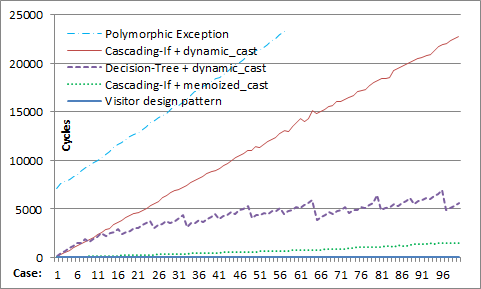
\includegraphics[width=0.47\textwidth]{DCast-vs-Visitors1.png}
  \caption{Type switching based on na\"ive techniques}
  \label{fig:DCastVis1}
\end{figure}

When the class hierarchy is not flat and has several levels, the above cascading-if can be replaced 
with a decision tree that tests base classes first and thus eliminates many of 
the derived classes from consideration. This approach is used by Emir to deal with 
type patterns in Scala~\cite[\textsection 4.2]{EmirThesis}. The intent is to 
replace a sequence of independent dynamic casts between classes that are far 
from each other in the hierarchy with nested dynamic casts between classes that 
are close to each other. Another advantage is the possibility to fail early: 
if the type of the subject does not match any of the clauses, we will not have to try all the cases. 
A flat hierarchy, which will likely be formed by the leaves in even a multi-level 
hierarchy, will not be able to benefit from this optimization and 
will effectively degrade to the above cascading-if. Nevertheless, when 
applicable, the optimization can be very useful and its benefits can be seen in
Figure~\ref{fig:DCastVis1} under ``Decision-Tree + dynamic\_cast''. The class 
hierarchy for this timing experiment formed a perfect binary tree with 
classes number 2*N and 2*N+1 derived from a class with number N. The structure 
of the hierarchy also explains the repetitive pattern of timings.

The above solution either in a form of cascading-if or as a decision tree can be 
significantly improved by lowering the cost of a single \code{dynamic_cast}. 
We devised an asymptotically constant version of this operator that we call
\code{memoized_cast} in \textsection\ref{sec:memcast}. As can be seen 
from the graph titled ``Cascading-If + memoized\_cast'', it speeds up the 
above cascading-if solution by a factor of 18 on average, as well as outperforms 
the decision-tree based solution with dynamic\_cast for a number of case clauses 
way beyond those that can happen in a reasonable program. 
We leave the discussion of the technique until 
\textsection\ref{sec:memcast}, while we keep it in the chart to give perspective on 
an even faster solution to dynamic casting. The slowest implementation in the 
chart based on exception handling facilities of C++ is discussed in 
\textsection\ref{sec:xpm}.

The approach of Gibbs and Stroustrup~\cite{FastDynCast} employs divisibility of numbers to obtain a 
tag allocation scheme capable of performing type testing in constant time. 
Extended with a mechanism for storing offsets required for this-pointer 
adjustments, the technique can be used for extremely fast dynamic casting on 
quite large class hierarchies. The idea is to allocate tags 
for each class in such a way that tag of a class D is divisible by a tag of a 
class B if and only if class D is derived from class B. For comparison purposes 
we hand crafted this technique on the above flat and binary-tree hierarchies and 
then redid the timing experiments from Figure~\ref{fig:DCastVis1} using the fast 
dynamic cast. The results are presented in Figure~\ref{fig:DCastVis2}. For 
reference purposes we retained ``Visitor Design Pattern'' and ``Cascading-If + 
memoized\_cast'' timings from Figure~\ref{fig:DCastVis1} unchanged. Note that 
the Y-axis has been scaled-up 140 times, which is why the slope of 
``Cascading-If + memoized\_cast'' timings is so much steeper.

\begin{figure}[htbp]
  \centering
    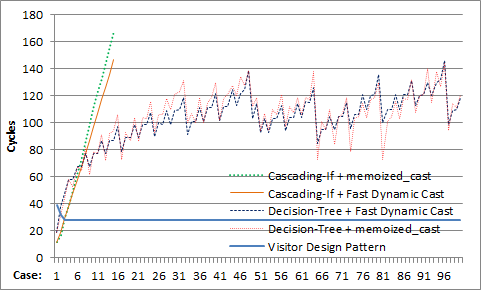
\includegraphics[width=0.47\textwidth]{DCast-vs-Visitors2.png}
  \caption{Type switching based on the fast dynamic cast of Gibbs and Stroustrup~\cite{FastDynCast}}
  \label{fig:DCastVis2}
\end{figure}

As can be seen from the figure the use of our memoized\_cast implementation can 
get close in terms of performance to the fast dynamic cast, especially 
when combined with decision trees. An important difference that cannot be seen 
from the chart, however, is that the performance of memoized\_cast is 
asymptotic, while the performance of fast dynamic cast is guaranteed. This 
happens because the implementation of memoized\_cast will incur an overhead of 
a regular dynamic\_cast call on every first call with a given most derived type. 
Once that class is memoized, the performance will remain as shown. Averaged over 
all calls with a given type we can only claim we are asymptotically as good as 
fast dynamic cast.

Unfortunately fast dynamic casting is not truly open to fully satisfy our 
checklist. The structure of tags required by the scheme limits the number of 
classes it can handle. A 32-bit integer is estimated to be able to represent 7 
levels of a class hierarchy that forms a binary tree (255 classes), 6 levels of 
a similar ternary tree hierarchy (1093 classes) or just one level of a hierarchy 
with 9 base classes -- multiple inheritance is the worst case scenario of the 
scheme that quickly drains its allocation possibilities. Besides, similarly to 
other tag allocation schemes, presence of class extensions in \emph{Dynamically Linked Libraries} (DLLs) will likely 
require an integration effort to make sure different DLLs are not reusing prime 
numbers in a way that might result in an incorrect dynamic cast.

A number of other constant-time techniques for class-membership testing is 
surveyed by Gil and Zibin~\cite[\textsection 4]{PQEncoding}. They are intended 
for type testing, and thus will have to be combined with decision trees 
for type switching, resulting in similar to fast dynamic cast performance. 
They too assume access to the entire class hierarchy at compile time and thus 
are not open.

In view of the predictably-constant dispatching overhead of the visitor design pattern, 
it is clear that any open solution that will have a non-constant dispatching 
overhead will have a poor chance of being adopted. Multi-way switch on 
sequentially allocated tags~\cite{Spuler94} was one of the few techniques that 
could achieve constant overhead, and thus compete with and even outperform visitors. 
Unfortunately the scheme has problems of its own that make it unsuitable for 
truly open type-switching and here is why.

%To better understand the problem let us look at some existing solutions to type 
%switching that we found to be used in practice. 

%From our experience on this project we have noticed that we can only compete 
%with visitors when switch statements are implemented with a jump table. As soon 
%as compiler was putting even a single branch into the decision tree of cases, 
%the performance was degraded significantly. From this perspective we do not 
%regard solutions based on decision trees as efficient, since they do not let us 
%compete compete with the visitors solution.

The simple scheme of assigning a unique tag per variant (instantiatable class 
here) will not pass our first question because the tags of base and derived 
classes will have to be different if the base class can be instantiated on its 
own. In other words we will not be able to land on a case label of a base class, while 
having a derived tag only. The already mentioned partitioning of tags of derived 
classes based on the classes in case clauses also will not help as it assumes 
knowledge of all the classes and thus fails extensibility through DLLs.

In practical implementations hand crafted for a specific class hierarchy, tags 
often are not chosen arbitrarily, but to reflect the subtyping relation of the 
underlying hierarchy. Switching on base classes in such a setting will typically 
involve a call to some function $f$ that converts derived class' tag into a base 
class' tag. An example of such a scheme would be having a certain bit in the tag 
set for all the classes derived from a given base class. Unfortunately this 
solution creates more problems than it solves.

First of all the solution will not be able to recognize an exceptional case 
where most of the derived classes should be handled as a base class, while a few 
should be handled specifically. Applying the function $f$ puts several different 
types into an equivalence class with their base type, making them 
indistinguishable from each other.

Secondly, the assumed structure of tags is likely to make the set of tags 
sparse, effectively forcing the compiler to use a decision tree instead of a jump 
table to implement the switch. Even though conditional jump is reported to be 
faster than indirect jump on many computer architectures~\cite[\textsection 
4]{garrigue-98}, this did not seem to be the case in our experiments. Splitting 
of a jump table into two with a condition, that was sometimes happening because 
of our case label allocation scheme, was resulting in a noticeable degradation of 
performance in comparison to a single jump table.

Besides, as was seen in the scheme of Gibbs and Stroustrup, the assumed 
structure of tags can also significantly decrease the number of classes a given 
allocation scheme can handle. It is also interesting to note that even though 
their scheme can be easily adopted for type switching with decision trees, it is 
not easily adoptable for type switching with jump tables: in order to obtain 
tags of base classes we will have to decompose the derived tag into primes and 
then find all the dividers of the tag present in case clauses.

To summarize, truly open and efficient type switching is a non-trivial problem. 
The approaches we found in the literature were either open or efficient, 
but not both. Efficient implementation was typically achieved by sealing the 
class hierarchy and using a jump table on sequential tags. Open implementations 
were resorting to type testing and decision trees, which was not efficient. 
We are unaware of any efficient tag allocation scheme that can be used in a 
truly open scenario.

%%%%%%%%%%%%%%%%%%%%%%%%%%%%%%%%%%%%%%5555

%\noindent
%We chose to give it a first-fit semantics in our library as it was resembling 
%pattern matching facilities of other languages and was the most intuitive. The 
%following code can be generated to implement it:
%
%\begin{lstlisting}
%if (D1* derived = dynamic_cast<D1*>(base)) { s1; } else
%if (D2* derived = dynamic_cast<D2*>(base)) { s2; } else
%...
%if (Dn* derived = dynamic_cast<Dn*>(base)) { sn; }
%\end{lstlisting}

%\noindent
%Note that leaving \code{else} out will effectively turn it into an all-fit 
%statement with enabled statements executed in lexicographical order.
%
%The above code is easy to understand but is extremely inefficient as for an 
%object of dynamic type $D_i$ we will have to perform $i-1$ dynamic casts that 
%fail first. The diagram below compares the times spent by visitors and the above 
%type switch statement to uncover the $i^{th}$ case. We postpone the discussion 
%of \code{memoized_cast} until section \textsection\ref{}, here we would only 
%like to notice that even though faster than the actual dynamic cast it also bears 
%a linear coefficient, not present in visitors.

\section{Solution for Polymorphic Classes}
\label{sec:copc}

Our handling of type switches for polymorphic and tagged encodings differs 
with each having its pros and cons described in details in \textsection\ref{sec:cmp}.
In this section we will concentrate on the truly open type switch for 
polymorphic encoding. The type switch for tagged encoding (\textsection\ref{sec:cotc}) 
is simpler and more efficient, however, making it open will eradicate its 
performance advantages. The difference in performance is the price we pay for 
keeping the solution open.  The core of the proposal relies on two key
aspects of C++ implementations:
\begin{enumerate}
\item a constant-time access to the virtual table pointer embedded in an object of
  dynamic class type;
\item injectivity of the relation between an object's inheritance path
  and the virtual table pointer extracted from that object.
\end{enumerate}

\subsection{Virtual Table Pointers}
\label{sec:vtp}

Before we discuss our solution we would like to talk about certain properties of 
the C++ run-time system that we rely on. In particular,
we show that under certain conditions the compiler cannot share 
the same virtual tables between different classes or subobjects of the same 
class. This allows us to use virtual table pointers to \emph{uniquely} identify 
the subobjects within the most derived class.

Strictly speaking, the C++ standard~\cite{C++0x} does not require implementations 
to use any specific technique (e.g. virtual tables) to implement virtual functions, 
however interoperability requirements have forced many compiler vendors to design a 
set of rules called Common Vendor Application Binary Interface (the C++ 
ABI)~\cite{C++ABI}. Most C++ compilers today follow these rules, with the 
notable exception of Microsoft Visual C++. The technique presented here will 
work with any C++ compiler that follows the C++ ABI. Microsoft's own ABI is not 
publically available and thus we cannot formally verify that it satisfies 
our requirements. Nevertheless, we did run numerous experiments with various 
class hierarchies and have sufficient confidence that our approach can be used 
in Visual C++. This is why we include experimental results for this compiler as 
well.

Besides single inheritance, which is supported by most object-oriented languages, 
C++ supports multiple-inheritance of two kinds: repeated and virtual (shared). 
\emph{Repeated inheritance} creates multiple independent subobjects of the same 
type within the most derived type. \emph{Virtual inheritance} creates only one 
shared subobject, regardless of the inheritance paths. Because of this 
peculiarity of the C++ type system it is not sufficient to talk only about the 
static and dynamic types of an object -- one has to talk about a 
\emph{subobject} of a certain static type accessible through a given inheritance 
path within a dynamic type.

\begin{figure}[tbp]
  \centering
    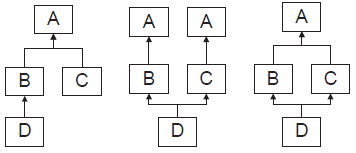
\includegraphics[width=0.47\textwidth]{Hierarchies.png}
  \caption{Single inheritance, repeated multiple inheritance and virtual multiple inheritance}
  \label{fig:hierarchy}
\end{figure}

\noindent
Note that the above picture portrais subobject relatedion, not the inheritance.

The notion of subobject has been formalized before~\cite{RF95,WNST06,RDL11}.
We follow here the presentation of Ramamanandro et al~\cite{RDL11}.

A base class subobject of a given complete object is represented by a pair 
$\sigma = \langle h,l\rangle$ with $h \in \{\mathrm{Repeated},\mathrm{Shared}\}$ representing the 
kind of inheritance (single inheritance is $\mathrm{Repeated}$ with one base class) and $l$ 
representing the path in a non-virtual inheritance graph.

A predicate $C\leftY\sigma\rightY A$ they introduce means that $\sigma$ 
designates a subobject of static type $A$ within the most derived object of 
type $C$.

A class that declares or inherits a virtual function is called a 
\emph{polymorphic class}~\cite[\textsection 10.3]{C++0x}. The C++ ABI in turn defines 
\emph{dynamic class} to be a class requiring a virtual table pointer (because it 
or its bases have one or more virtual member functions or virtual base classes). 
A polymorphic class is thus a dynamic class by definition.

A \emph{virtual table pointer} (vtbl-pointer) is a member of object's layout 
pointing to a virtual table. A \emph{virtual table} is a table of information used 
to dispatch virtual functions, access virtual base class subobjects, and to 
access information for \emph{RunTime Type Identification} (RTTI). Because of repeated
inheritance, an object of given type may have several vtbl-pointers in it. Each 
such pointer corresponds to one of the polymorphic base classes. Given an object 
$a$ of static type $A$ that has $k$ vtbl-pointers in it, we will use the same 
notation we use for regular fields to refer them: $a.\textit{vtbl}_i$.

A \emph{primary base class} for a dynamic class is the unique base class (if any) 
with which it shares the virtual table pointer at offset 0. The data layout 
procedure for non-POD types described in \textsection2.4 of the C++ ABI~\cite{C++ABI} 
requires dynamic classes either to allocate vtable pointer at offset 0 or share 
the virtual table pointer from its primary base class, which is by definition at 
offset 0. For our purpose this means that we can rely on a virtual table pointer 
always being present at offset 0 for all dynamic classes, and thus for all polymorphic 
classes.

\begin{lemma}
In an object layout that adheres to the C++ ABI, a polymorphic class always has a 
virtual table pointer at offset 0.
\label{lem:vtbl}
\end{lemma}

\noindent
Knowing how to extract a vtbl-pointer as well as that all the objects of the 
same most derived type share the same vtbl-pointers, the idea is to use their 
values to uniquely identify the type and subobject within it. Unfortunately 
nothing in the C++ ABI states these pointers should be unique. A popular 
optimization technique lets the compiler share the virtual table of a derived 
class with its primary base class as long as the derived class that does not 
override any virtual methods. Use of such optimization will violate the 
uniqueness of vtbl-pointers; however, we show below that in the presense of 
RTTI, a C++ ABI-compliant implementation is guaranteed to have different values 
of vtbl-pointers in different subobjects.

%C++ standard requires an argument of \code{dynamic_cast} to be a pointer to or 
%an lvalue of a polymorphic type when performing \emph{downcast} -- a cast from 
%base to derived~\cite[\textsection 5.2.7-6]{C++0x}. We can thus always safely 
%extract virtual table pointer from offset 0 of any valid argument to 
%\code{dynamic_cast}.

%Similarly, each class that has virtual member functions or virtual bases has an 
%associated set of virtual tables. There may be multiple virtual tables for a 
%particular class, if it is used as a base class for other classes. However, the 
%virtual table pointers within all the objects (instances) of a particular 
%most-derived class point to the same set of virtual tables.

The exact content of the virtual table is not important for our discussion, but 
we would like to point out a few fields in it. The following definitions are 
copied verbatim from the C++ ABI~\cite[\textsection 2.5.2]{C++ABI}:

\begin{itemize}
\setlength{\itemsep}{0pt}
\setlength{\parskip}{0pt}
\item The \emph{typeinfo pointer} points to the typeinfo object used for RTTI. 
      It is always present.  
\item The \emph{offset to top} holds the displacement to the top of the object 
      from the location within the object of the virtual table pointer that 
      addresses this virtual table, as a \code{ptrdiff_t}. It is always present.
\item \emph{Virtual Base (vbase) offsets} are used to access the virtual bases 
      of an object. Such an entry is added to the derived class object address 
      (i.e. the address of its virtual table pointer) to get the address of a 
      virtual base class subobject. Such an entry is required for each virtual 
      base class.
\end{itemize}

\noindent
Given a virtual table pointer \code{vtbl}, we will refer to these fields as 
\code{rtti(vtbl)}, \code{off2top(vtbl)} and \code{vbase(vtbl)} respectively. 
We will also assume presence of a function $\mathit{offset}(\sigma)$ that defines the 
offset of the base class identified by the end of the path $\sigma$ within a 
class identified by its first element.

\begin{theorem}
In an object layout that adheres to the C++ ABI with present runtime type 
information, the equality of virtual table pointers of two objects of the same 
static type implies that they both belong to subobjects with the same 
inheritance path in the same most-derived type.
\begin{eqnarray*}
    \forall a_1, a_2 : A\ |\ a_1\in C_1\leftY\sigma_1\rightY A \wedge a_2\in C_2\leftY\sigma_2\rightY A \\
    a_1.\textit{vtbl}_i = a_2.\textit{vtbl}_i \Rightarrow C_1 = C_2 \wedge \sigma_1 = \sigma_2
\end{eqnarray*}
\label{thm:vtbl}
\end{theorem}
\begin{proof}
Let us assume first $a_1.\textit{vtbl}_i = a_2.\textit{vtbl}_i$ but $C_1 \neq C_2$. In this case we 
have \code{rtti}$(a_1.\textit{vtbl}_i) = $\code{rtti}$(a_2.\textit{vtbl}_i)$. By definition 
\code{rtti}$(a_1.\textit{vtbl}_i) = C_1$ while \code{rtti}$(a_2.\textit{vtbl}_i) = C_2$, which 
contradicts that $C_1 \neq C_2$. Thus $C_1 = C_2 = C$.

Let us assume now that $a_1.\textit{vtbl}_i = a_2.\textit{vtbl}_i$ but $\sigma_1 \neq \sigma_2$. 
Let $\sigma_i=\langle h_i,l_i\rangle,i=1,2$ 

If $h_1 \neq h_2$ then one of them refers to a virtual base while the other to a 
repeated one. Assuming $h_1$ refers to a virtual path, \code{vbase}$(a_1.\textit{vtbl}_i)$ 
has to be defined inside the vtable according to the ABI, while 
\code{vbase}$(a_2.\textit{vtbl}_i)$ -- should not. This would contradict again that both 
$vtbl_i$ refer to the same virtual table.

We thus have $h_1 = h_2 = h$. If $h = \mathrm{Shared}$ then there is only one path to 
such $A$ in $C$, which would contradict $\sigma_1 \neq \sigma_2$. 
If $h = \mathrm{Repeated}$ then we must have that $l_1 \neq l_2$. In this case let $k$ be 
the first position in which they differ: 
$l_1^j=l_2^j \forall j<k \wedge l_1^k\neq l_2^k$. Since our class $A$ is a base 
class for classes $l_1^k$ and $l_2^k$, both of which are in turn base classes of 
$C$, the object identity requirement of C++ requires that the relevant subobjects 
of type $A$ have different offsets within class $C$: 
$\mathit{offset}(\sigma_1)\neq \mathit{offset}(\sigma_2)$ However 
$\mathit{offset}(\sigma_1)=$\code{off2top}$(a_1.\textit{vtbl}_i)=$\code{off2top}$(a_2.\textit{vtbl}_i)=\mathit{offset}(\sigma_2)$ 
since $a_1.\textit{vtbl}_i = a_2.\textit{vtbl}_i$, which contradicts that the offsets are different.
\end{proof}

\noindent
Conjecture in the other direction is not true in general as there may be 
duplicate virtual tables for the same type present at run-time. This happens in 
many C++ implementations in the presence of DLLs as the same class compiled into 
executable and into a DLL it loads may have identical virtual tables inside the 
executable's and DLL's binaries.

Note also that we require both static types to be the same. Dropping this 
requirement and saying that equality of vtbl-pointers also implies equality of 
the static types is not true in general because a derived class will share the 
vtbl-pointer with its primary base class (see Lemma~\ref{lem:vtbl}). The theorem 
can be reformulated, however, stating that one static type will necessarily have 
to be a subtype of the other. The current formulation is sufficient for our 
purposes, while reformulation would have required more elaborate discussion of 
the algebra of subobjects~\cite{RDL11}, which we touch only briefly.

\begin{corollary}
Results of \code{dynamic_cast} can be reapplied to a different instance from 
within the same subobject. 

$\forall A,B \forall a_1, a_2 : A\ |\ a_1.\textit{vtbl}_i = a_2.\textit{vtbl}_i \Rightarrow$ \\
\code{dynamic_cast<B>}$(a_1).\textit{vtbl}_j = $\code{dynamic_cast<B>}$(a_2).\textit{vtbl}_j \vee$ \\
\code{dynamic_cast<B>}$(a_1)$ throws $\wedge$ \code{dynamic_cast<B>}$(a_2)$ throws.
\label{crl:vtbl}
\end{corollary}

\noindent
During construction and deconstruction of 
an object, the value of a given vtbl-pointer may change. In particular, 
that value will reflect the dynamic type of the object to be the type of the 
fully constructed part only. However, this does not affect our reasoning, as during 
such transition we also treat the object to have the type of its fully 
constructed base only. Such interpretation is in line with the C++ semantics for 
virtual function calls and the use of RTTI during construction and destruction of an 
object. Once the complete object is fully constructed, the value of the 
vtbl-pointer will remain the same for the lifetime of the object.

\subsection{Memoization Device}
\label{sec:memdev}

Let us look at a slightly more general problem than type switching. Consider a 
generalization of the switch statement that takes predicates on a subject as its 
clauses and executes the first statement $s_i$ whose predicate is enabled: 

\begin{lstlisting}
switch (x)
{
    case P1(x): s1;
    ...
    case Pn(x): sn;
}
\end{lstlisting}

\noindent
Assuming that predicates depend only on $x$ and nothing else as well as that 
they do not involve any side effects, we can be sure that the next time we come 
to such a switch with the same value, the same predicate will be enabled 
first. Thus, we would like to avoid evaluating predicates and jump straight to 
the statement it guards. In a way we would like the switch to  memoize which 
case is enabled for a given value of $x$.

The idea is to generate a simple cascading-if statement interleaved with jump 
targets and instructions that associate the original value with enabled target. 
The code before the statement looks up whether the association for a given value 
has already been established, and, if so, jumps directly to the target; otherwise 
the sequential execution of the cascading-if is started. To ensure 
that the actual code associated with the predicates remains unaware of this 
optimization, the code preceeding it after the target must re-establish any 
invariant guaranteed by sequential execution (\textsection\ref{sec:vtblmem}).

The above code can easily be produced in a compiler setting, but producing it in 
a library setting is a challenge. Inspired by Duff's Device~\cite{Duff}, 
we devised a construct that we call \emph{Memoization Device} that does just 
that in standard C++:

\begin{lstlisting}
typedef decltype(x) T;
static std::unordered_map<T,int> jump_target_map;

switch (int& target = jump_target_map[x])
{
default: // entered when we have not seen x yet
    if (P1(x)) { target = 1;   case 1: s1; } else 
    if (P2(x)) { target = 2;   case 2: s2; } else
 ...
    if (Pn(x)) { target = @$n$@; case @$n$@: sn; } else
                target = @$n+1$@;
case @$n+1$@: // none of the predicates is true on x
}
\end{lstlisting}

\noindent
The static \code{jump_target_map} hash table will be allocated upon first entry 
to the function. The map is initially empty and according to its logic, 
request for a key $x$ not yet in the map will result in allocation of a 
new entry with its associated data default initialized (to 0 for int). Since 
there is no case label 0 in the switch, the default case will be taken, which, in 
turn, will initiate sequential execution of the interleaved cascading-if 
statement. Assignments to \code{target} effectively establish association 
between value $x$ and corresponding predicate, since \code{target} is just a 
reference to \code{jump_target_map[x]}. The last assignment records absence of 
enabled predicates for the value.

The sequential execution of the cascading-if statement will keep checking 
predicates $P_j(x)$ until the first predicate $P_i(x)$ that returns true. By 
assigning $i$ to \code{target} we will effectively associate $i$ with $x$ since 
\code{target} is just a reference to \code{jump_target_map[x]}. This association 
will make sure that the next time we are called with the value $x$ we will jump 
directly to the label $i$. When none of the predicates returns true, we will 
record it by associating $x$ with $N+1$, so that the next time we can jump 
directly to the end of the switch on $x$. 

The above construct effectively gives the entire statement first-fit semantics. 
In order to evaluate all the statements whose predicates are true, and thus 
give the construct all-fit semantics, we might want to be able to preserve the 
fall-through behavior of the switch. In this case we can still skip the initial 
predicates returning false and start from the first successful one. This can be 
easily achieved by removing all else statements and making if-statements 
independent as well as wrapping all assignments to \code{target} with a condition, 
to make sure only the first successful predicate executes it:

\begin{lstlisting}
    if (Pi(x)) { if (target == 0) target = @$i$@; case @$i$@: si; }
\end{lstlisting}

\noindent
Note that the protocol that has to be maintained by this structure does not 
depend on the actual values of case labels. We only require them to be 
different and include a predefined default value. The default clause can be 
replaced with a case clause for the predefined value, however keeping the default  
clause results in a faster code. A more important performance consideration is to 
keep the values close to each other. Not following this rule might result in a 
compiler choosing a decision tree over a jump table implementation of the 
switch, which in our experience significantly degrades the performance.

The first-fit semantics is not an inherent property of the memoization device however. 
Assuming that the conditions are either mutually exclusive or imply one another, we 
can build a decision-tree-based memoization device that will effectively have 
\emph{most-specific} semantics -- an analog of best-fit semantics in predicate 
dispatching~\cite{ErnstKC98}.

Imagine that the predicates with the numbers $2i$ and $2i+1$ are mutually exclusive and 
each imply the value of the predicate with number $i$ i.e. $\forall x \in \mathsf{Domain}(P)$
\begin{eqnarray*}
P_{2i+1}(x)\rightarrow P_i(x) \wedge P_{2i}(x)\rightarrow P_i(x) \wedge \neg(P_{2i+1}(x) \wedge P_{2i}(x))
\end{eqnarray*}
\noindent
The following decision-tree based memoization device will execute the statement 
$s_i$ associated with the \emph{most-specific} predicate $P_i$ (i.e. the 
predicate that implies all other predicates true on $x$) that evaluates to true or will 
skip the entire statement if none of the predicates is true on $x$.

\begin{lstlisting}
switch (int& target = jump_target_map[x])
{
default:
    if (P1(x)) {
        if (P2(x)) {
            if (P4(x)) { target = 4; case 4: s4; } else
            if (P5(x)) { target = 5; case 5: s5; } 
            target = 2; case 2: s2;
        } else
        if (P3(x)) {
            if (P6(x)) { target = 6; case 6: s6; } else
            if (P7(x)) { target = 7; case 7: s7; } 
            target = 3; case 3: s3;
        }
        target = 1; case 1: s1;
    } else {
        target = 0; case 0:   ;
    }
}
\end{lstlisting}

\noindent
An example of predicates that satisfy this condition are class membership tests
where the truth of a predicate that tests membership in a derived class implies 
the truth of a predicate that tests membership in its base class. Our library 
solution prefers the simpler cascading-if approach only because the necessary 
structure of the code can be laid out directly with macros. A compiler solution 
will use the decision-tree approach whenever possible to lower the cost of the 
first match from linear in case's number to logarithmic as seen in Figure\ref{fig:DCastVis1}.

When the predicates do not satisfy the implication or mutual exclusion properties 
mentioned above, a compiler of a language based on predicate dispatching would 
typically issue an ambiguity error. Some languages might choose to resolve it 
according to lexical or some other ordering. In any case, the presence of 
ambiguities or their resolution has nothing to do with memoization device 
itself. The latter only helps optimize the execution once a particular choice of 
semantics has been made and code implementing it has been laid out.

The main advantage of the memoization device is that it can be built around 
almost any code, providing that we can re-establish the invariants, guaranteed 
by sequential execution. Its main disadvantage is the size of the hash table 
that grows proportionally to the number of different values seen. Fortunately, 
the values can often be grouped into equivalence classes, such that values in 
the same class do not change the predicate. The map can then associate the 
equivalence class of a value with a target instead of associating the value with 
it. The next subsection does exactly that for polymorphic objects.

\subsection{Vtable Pointer Memoization}
\label{sec:vtblmem}

The memoization device can almost immediately be used for multi-way type testing by 
using \code{dynamic_cast<Di>} as a predicate $P_i$. This cannot be considered a 
type switching solution, however, as one would expect to also have a reference 
to the uncovered type. Using a \code{static_cast<Di>} upon successful type test 
would have been a solution if we did not have multiple inheritance. It certainly 
can be used as such in languages with only single inheritance. For the fully 
functional C++ solution, we combine the memoization device with the properties 
of virtual table pointers into a \emph{Vtable Pointer Memoization} technique.

We saw that vtbl-pointers uniquely determine the subobject within an object 
(Theorem~\ref{thm:vtbl}), while the result of a \code{dynamic_cast} can be reapplied 
from the same subobject (Corollary~\ref{crl:vtbl}). The idea is thus to group 
all the objects according to the value of their vtbl-pointer and associate both 
target and the required offset with it through memoization device:

\begin{lstlisting}
typedef std::pair<ptrdiff_t,size_t> type_switch_info;
static std::unordered_map<intptr_t, type_switch_info> jump_target_map;
intptr_t          vtbl = *reinterpret_cast<const intptr_t*>(p);
type_switch_info& info = jump_target_map[vtbl];
const void*       tptr; 
switch (info.second) ...
\end{lstlisting}

\noindent
We use the virtual table pointer extracted from a polymorphic object pointed to 
by \code{p} as a key for association. The value stored along the key in 
association now keeps both: the target for the switch as well as a memoized 
offset for dynamic cast. 

The code for the $i^{th}$ case now evaluates the required offset on the first 
entry and associates it along the target with the vtbl-pointer of the subject.
The call to \code{adjust_ptr<Di>} re-establishes the invariant that 
\code{matched} is a properly-casted reference to type \code{Di} of the subject 
\code{p}.
%The condition of the inner if-statement is only needed to implement the 
%sequential all-fit semantics and can be removed when fall-through behavior is 
%not required.

\begin{lstlisting}
    if (tptr = dynamic_cast<const Di*>(p)) {
        if (info.second == 0) { // supports fall-through
            info.first  = intptr_t(tptr)-intptr_t(p); // offset
            info.second = @$i$@; // jump target
        }
case @$i$@: // @$i$@ is a constant here - clause's position in switch
        auto matched = adjust_ptr<Di>(p,info.first); 
        si;
    }
\end{lstlisting}

\noindent
The main condition remains the same. We keep checking for the first initialization 
because we allow fall-through semantics here, letting the user break from the 
switch when needed. Upon first entry we compute the offset that the dynamic cast 
performed and save it together with target associated to the virtual table 
pointer. On the next iteration we will jump directly to the case label and 
restore the invariant of \code{matched} being a properly-casted reference to the 
derived object.

The use of dynamic cast makes a huge difference in comparison to the use of 
static cast we dismissed above. First of all the C++ type system is much more 
restrictive about the static cast and many cases where it is not allowed can 
still be handled by dynamic cast. Examples of these include downcasting from an 
ambiguous base class or cross-casting between unrelated base classes.

An important benefit we get from this optimization is that we do not store the 
actual values (pointers to objects) in the hash table anymore, but group them 
into equivalence classes based on their virtual table pointers. The number of 
such pointers in a program is always bound by $O(|A|)$, where $A$ represents the 
static type of an object, while $|A|$ represents the number of classes directly 
or indirectly derived from $A$. The linear coefficient hidden in big-o notation 
reflects possibly multiple vtbl-pointers in derived classes due to the use of 
multiple inheritance.

\begin{figure}[htbp]
  \centering
    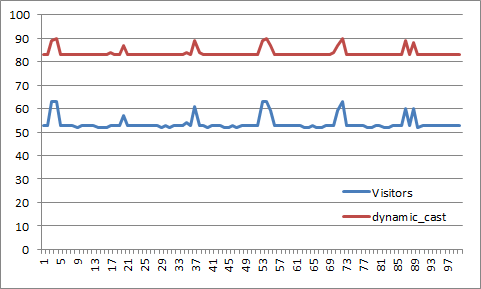
\includegraphics[width=0.47\textwidth]{DCast-vs-Visitors3.png}
  \caption{Time to uncover i\textsuperscript{th} case. X-axis - case i; Y-axis - cycles per iteration}
  \label{fig:DCastVis3}
\end{figure}

The most important benefit of this optimization, however, is the constant time 
on average used to dispatch each of the case clauses, regardless of their 
position in the type switch. The net effect of this optimization can be seen in Figure~\ref{fig:DCastVis3}. 
We can see that the time does not increase with the position of the case we are 
handling. The spikes represent activities on computer during measurement and are 
present in both measurements. 
The constant time on average comes from the average complexity 
of accessing an element in an \code{unordered_map}, while its worst complexity can 
be proportional to the size of the map. We show in the next section, however, 
that most of the time we will be bypassing traditional access to elements of the 
map, because, as-is, the type switch is still about 50\% slower than the visitor 
design pattern.

Note that we can apply the reasoning of \textsection\ref{sec:memdev} and change 
the first-fit semantics of the resulting match statement into a best-fit 
semantics simply by changing the underlying cascading-if structure with decision 
tree. A compiler implementation of a type switch based on Vtable Pointer 
Memoization will certainly take advantage of this optimization to cut down the 
cost of the first run on a given vtbl-pointer, when the actual memoization happens.

\subsubsection{Structure of Virtual Table Pointers}
\label{sec:sovtp}

Virtual table pointers are not entirely random addresses in memory and have 
certain structure when we look at groups of those that are associated with 
classes related by inheritance. Let us first look at some vtbl pointers that 
were present in some of our tests. The 32-bit pointers are shown in binary form 
(lower bits on the right) and are sorted in ascending order:

\begin{verbatim}
00000001001111100000011001001000
00000001001111100000011001011100
00000001001111100000011001110000
 ...
00000001001111100000011111011000
00000001001111100000011111101100
\end{verbatim}

Virtual table pointers are not constant values and are not even guaranteed to be 
the same between different runs of the same application. Techniques like 
\emph{address space layout randomization} or simple \emph{rebasing} of the entire 
module are likely to change these values. The relative distance between them is 
likely to remain the same though as long as they come from the same module.

Comparing all the vtbl pointers that are coming through a given match statement 
we can trace ar run time the set of bits in which they do and do not differ. 
For the above example it may look as \texttt{00000001001111100000X11XXXXXXX00} 
where positions marked with X represent bits that are different in some vtbl 
pointers.

When a DLL is loaded it may have its own copy of vtables for classes also used 
in other modules as well as vtables for classes it introduces. Comparing 
similarly all vtbl pointers coming only from this DLL we can get a different 
pattern \\ \texttt{01110011100000010111XXXXXXXXX000} and when compared over all 
the loaded modules the pattern will likely becomes something like 
\texttt{0XXX00X1X0XXXXXX0XXXXXXXXXXXXX00}.

The common bits on the right come from the virtual table size and alignment 
requirements, and, depending on compiler, configuration, and class hierarchy could 
easily vary from 2 to 6 bits. Because the vtbl-pointer under the C++ ABI points into 
an array of function pointers, the alignment requirement of 4 bytes for those 
pointers on a 32-bit architecture is what makes at least the last 2 bits to be 0. 
For our purpose the exact number of bits on the right is not important as we 
evaluate this number at run time based on vtbl-pointers seen so far. Here we only 
would like to point out that there would be some number of common bits on the 
right.

Another observation we made during our experiments with the vtbl-pointers of various 
existing applications was that the values of the pointers where changing more 
frequently in the lower bits than in the higher ones. We believe that this was 
happening because programmers tend to group multiple derived classes in the same 
translation unit so the compiler was emitting virtual tables for them close to 
each other as well. 

Note that derived classes that do not introduce their own virtual functions 
(even if they override some existing ones) are likely to have virtual tables of 
the same size as their base class. Even when they do add new virtual functions, 
the size of their virtual tables can only increase relative to their base 
classes. This is why the difference between many consecutive vtbl-pointers that 
came through a given match statement was usually constant or very slightly 
different.

The changes in higher bits were typically due to separate compilation and 
especially due to dynamically loaded modules. When a DLL is loaded, it may have 
its own copies of vtables for classes that are also used in other modules, in addition to 
vtables for classes it introduces. Comparing all vtbl-pointers coming only from 
that DLL we can get a different pattern \texttt{01110011100000010111XXXXXXXXX000} 
and when compared over all the loaded modules the pattern will likely become 
something like \texttt{0XXX00X1X0XXXXXX0XXXXXXXXXXXXX00}. Overall they were not 
changing the general tendency we saw: smaller bits were changing more frequently 
than larger ones, with the exception of the lowest common bits, of course.

These observations made virtual table pointers of classes related by inheritance 
ideally suitable for indexing -- the values obtained by throwing away the common 
bits on the right were compactly distributed in small disjoint ranges. We use 
those values to address a cache built on top of the hash table in order to 
eliminate a hash table lookup in most of the cases.  The important 
guarantee about the validity of the cached hash table references comes from the 
C++0x standard, which states that ``insert and emplace members shall not affect 
the validity of references to container elements''~\cite[\textsection 
23.2.5(13)]{C++0x}. 

Depending on the number of actual collisions that happen in the cache, our 
vtable pointer memoization technique can come close to, and even outperform, the 
visitor design pattern. The numbers are, of course, averaged over many runs as 
the first run on every vtbl-pointer will take an amount of time as shown in 
Figure\ref{fig:DCastVis1}. We did however test our technique on real code and 
can confirm that it does perform well in the real-world use cases.

The information about jump targets and necessary offsets is just an example of 
information we might want to be able to associate with, and access via, virtual 
table pointers. Our implementation of \code{memoized_cast} from 
\textsection\ref{sec:memcast} effectively reuses this general data structure with 
a different type of element values. We thus created a generic reusable class 
\code{vtblmap<T>} that maps vtbl-pointers to elements of type T. We will refer 
to the combined cache and hash-table data structure, extended with the logic for 
minimizing conflicts presented below, as a \emph{vtblmap} data structure.

\subsubsection{Minimization of Conflicts}
\label{sec:moc}

The small number of cycles that the visitor design pattern needs to uncover a 
type does not let us put too sophisticated cache indexing mechanisms into the 
critical path of execution. This is why we limit our indexing function to shifts 
and masking operations as well as choose the size of the cache to be a power of 2.

Throughout this section by \emph{collision} we will call a run-time condition in 
which the cache entry of an incoming vtbl pointer is occupied by another vtbl-pointer.
Collision requires vtblmap to fetch the data associated with the new 
vtbl-pointer from a slower hash-table and, under certain conditions, reconfigure 
cache for better performance. By \emph{conflict} we will call a different 
run-time condition under which given cache configuration maps two or more vtbl 
pointers to the same cache location. Presence of conflict does not necessarily 
imply presence of collisions, but collisions can only happen when there is a 
conflict. In the rest of this section we devise a mechanism that tries to 
minimize the amount of conflicts in a hope that it will also decrease the amount 
of actual collisions.

Given $n$ vtbl-pointers we can always find a cache size that will render no 
conflicts between them. The necessary size of such a cache, however, can be too 
big to justify the use of memory. This is why, in our current implementation, we 
always consider only 2 different cache sizes: $2^k$ and $2^{k+1}$ where 
$2^{k-1} < n \leq 2^k$. This guarantees that the cache size is never more than 4 
times bigger than the minimum required cache size.

During our experiments, we noticed that often the change in the smallest 
different bit happens only in a few vtbl-pointers, which was effectively 
cutting the available cache space in half. To overcome this problem, we let the 
number of bits by which we shift the vtbl-pointer vary further and compute it in 
a way that minimizes the number of conflicts.

To avoid doing any computations in the critical path, \code{vtblmap} only 
recomputes the optimal shift and the size of the cache when an actual collision 
happens. In order to avoid constant recomputations when conflicts are unavoidable, 
we add an additional restriction of only reconfiguring the optimal parameters if 
the number of vtbl-pointers in the \code{vtblmap} has increased since the last 
recomputation. Since the number of vtbl-pointers is of the order $O(|A|)$, where 
$A$ is the static type of all vtbl-pointers coming through a \code{vtblmap}, the 
restriction assures that reconfigurations will not happen infinitely often.

To minimize the number of recomputations even further, our library communicates 
to the \code{vtblmap}, through its constructor, the number of case clauses in 
the underlying match statement. We use this number as an estimate of the expected 
size of the \code{vtblmap} and pre-allocate the cache according to this estimated 
number. The cache is still allowed to grow based on the actual number of 
vtbl-pointers that comes through a \code{vtblmap}, but it never shrinks from the
initial value. This improvement significantly minimizes the number of collisions 
at early stages, as well as the number of possibilities we have to consider 
during reconfiguration.

The above logic of \code{vtblmap} always chooses the configuration that renders 
no conflicts, when such a configuration is possible during recomputation of 
optimal parameters. When this is not possible, it is natural to prefer collisions 
to happen on less-frequent vtbl-pointers.

We studied the frequency of vtbl-pointers that come through various match statements
of a C++ pretty-printer that we implemented on top of the Pivot 
framework~\cite{Pivot09} using our pattern-matching library. We ran the 
pretty-printer on a set of C++ standard library headers and then ranked all the  
classes from the most-frequent to the least-frequent ones, on average. The 
resulting probability distribution is shown with a thicker line in 
Figure\ref{fig:PowerLaw}.

\begin{figure}[htbp]
  \centering
    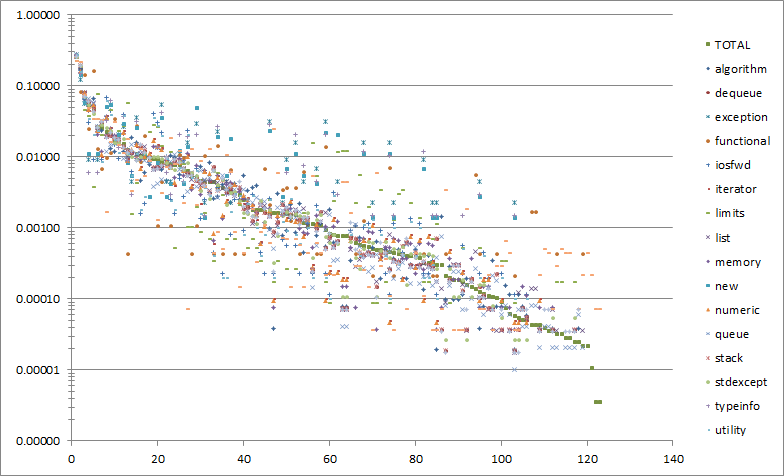
\includegraphics[width=0.47\textwidth]{std-lib-power-law-distributions.png}
  \caption{Probability distribution of various nodes in Pivot framework}
  \label{fig:PowerLaw}
\end{figure}

Note that Y-Axis is using logarithmic scale, suggesting that the resulting 
probability has power-law distribution. This is likely to be a specifics of our 
application, nevertheless, the above picture demonstrates that frequency of certain 
classes can be larger than the overall frequency of all the other classes. In 
our case, the two most frequent classes were representing the use of a variable in 
a program, and their combined frequency was larger than the frequency of all the 
other nodes. Naturally, we would like to avoid conflicts on such classes in the 
cache, when possible.

Let us assume that a given \code{vtblmap} contains a set of vtbl pointers 
$V = \{v_1, ... , v_n\}$ with known probabilities $p_i$ of occuring. For a cache 
of size $2^k$ and a shift by $l$ bits we get a cache-indexing function 
$f_{lk} : V \rightarrow [0..2^k-1]$ defined as $f_{lk}(v_i) = (v_i \gg l) \& (2^k-1)$.
To calculate the probability of conflict for a given $l$ and $k$ parameters, let 
us consider $j^{th}$ cache cell and a subset $V^j_{lk}=\{v \in V | f_{lk}(v)=j\}$. 
When the size of this subset $m=|V^j_{lk}|$ is greater than 1, we have a 
potential conflict as subsequent request for a vtbl pointer $v''$ might be 
different from the vtbl pointer $v'$ currenly stored in the cell $j$. Within the 
cell only the probability of not having a conflict is the probability of both 
values $v''$ and $v'$ be the same:
\begin{eqnarray*}
P(v''=v')=\sum\limits_{v_i \in V^j_{lk}}P(v''=v_i)P(v'=v_i)=\sum\limits_{v_i \in V^j_{lk}}P^2(v_i|V^j_{lk})=\\
=\sum\limits_{v_i \in V^j_{lk}}\frac{P^2(v_i)}{P^2(V^j_{lk})}=
\sum\limits_{v_i \in V^j_{lk}}\frac{p_i^2}{(\sum\limits_{v_{i'} \in V^j_{lk}}p_{i'})^2}=
\frac{\sum\limits_{v_i \in V^j_{lk}}p_i^2}{(\sum\limits_{v_{i} \in V^j_{lk}}p_{i})^2}
\end{eqnarray*}

The probability of having a conflict among the vtbl pointers of a given cell is 
thus one minus the above value:

\begin{eqnarray*}
P(v''\neq v')=1-\frac{\sum\limits_{v_i \in V^j_{lk}}p_i^2}{(\sum\limits_{v_{i} \in V^j_{lk}}p_{i})^2}
\end{eqnarray*}

To obtain probability of conflict given any vtbl pointer and not just the one 
from a given cell we need to sum up the above probabilities of conflict within a 
cell multiplied by the probability of vtbl pointer fall into that cell:

\begin{eqnarray*}
P_{lk}^{conflict}=\sum\limits_{j=0}^{2^k-1}P(V^j_{lk})(1-\frac{\sum\limits_{v_i \in V^j_{lk}}p_i^2}{(\sum\limits_{v_{i} \in V^j_{lk}}p_{i})^2})=\\
=\sum\limits_{j=0}^{2^k-1}(\sum\limits_{v_{i} \in V^j_{lk}}p_{i})(1-\frac{\sum\limits_{v_i \in V^j_{lk}}p_i^2}{(\sum\limits_{v_{i} \in V^j_{lk}}p_{i})^2})
\end{eqnarray*}

Our reconfiguration algorithm then iterates over possible values of $l$ and $k$ 
and chooses those that minimize the overal probability of conflict $P_{lk}^{conflict}$.
The only data still missing are the actual probabilities $p_i$ used by the above 
formula. They can be approximated in many different ways.

Besides probability distribution on all the tests, Figure~\ref{fig:PowerLaw} 
shows probabilities of a given node on each of the tests. The X-Axis in this 
case represents the ordering of all the nodes according to their overall rank 
of all the tests combined. As can be seen from the picture, the shape of each 
specific test's distribution still mimics the overal probability distribution. 
With this in mind we can simply let the user assign probabilities to each of the 
classes in the hierarchy and use these values during reconfiguration. The 
practical problem we came accross with this solution was that we wanted these 
probabilities be inheritable as Pivot separates interface and implementation 
classes and we prefered the user to define them on interfaces rather than on 
implementation classes. The easiest way to do so wast to write a dedicated 
function that would return the probabilities using a match statement. 
Unfortunately such a function will introduce a lot of overhead as it will 
ideally only be used very few times (since we try to minimize the amount of 
reconfiguration) and thus not be using memoized jumps but rather slow 
cascading-if.

A simpler and likely more precise way of estimating $p_i$ would be to count 
frequencies of each vtbl pointers directly inside the \code{vtblmap}. This 
introduces an overhead of an increment into the critical path of execution, but 
according to our tests was only degrading the overal performance by 1-2\%.
Instead, it was compensating with a smaller amount of conflicts and thus a 
potential gain of performance. We leave the choice of whether the library should 
count frequencies of each vtbl pointer to the user of the library as the 
concrete choice may be to advantage on some class hierarchies and to 
disadvantage on others.

Figure~\ref{fig:Collisions} compares the amount of collisions when frequency 
information is and is not used. The data was gathered from 312 tests on multiple 
match statements present in Pivot's C++ pretty printer when it was ran over 
standard library headers. In 122 of these test both schemes had 0 conflicts and 
these tests are thus not shown on the graph. The remaining tests where ranked by 
the amount of conflicts in the scheme that does not utilize frequency information.

\begin{figure}[htbp]
  \centering
    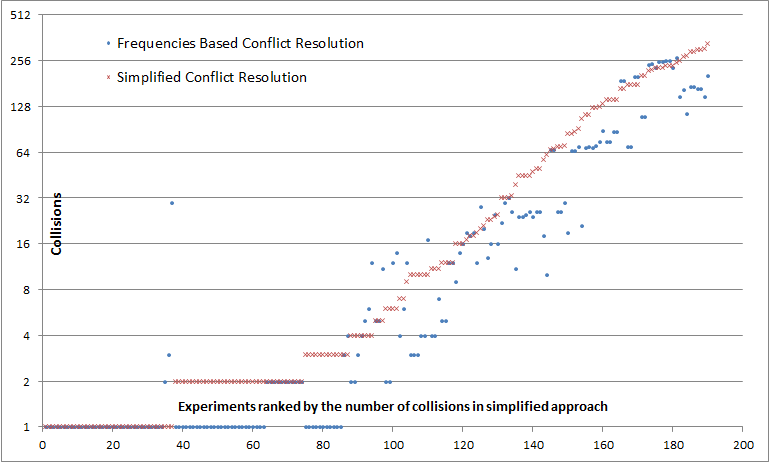
\includegraphics[width=0.47\textwidth]{CollisionsWithAndWithoutFrequencies.png}
  \caption{Decrease in number of collisions when probabilities of nodes are taken into account}
  \label{fig:Collisions}
\end{figure}

As can be seen from the graph, both schemes render quite low amount of 
collisions given that there was about 57000 calls in the rightmost test having 
the largest amount of conflicts. Taking into account that the Y-axis has 
logarithmic scale, the use of frequency information in many cases decreased the 
amount of conflicts by a factor of 2. The handfull of cases where the use of 
frequency increased the number of conflicts can be explained by the fact that 
the optimal values are not recomputed after each conflict, but after several 
conflicts and only if the amount of vtbl pointers in the vtblmap increased. These 
extra conditions sacrify optimality of parameters at any given time for the amount 
of times they are recomputed. By varying the number of conflicts we are willing 
to tolerate before reconfiguration we can decrease the number of conflicts by 
increasing the amount of recomputations and vise versa. From our experience, 
however, we saw that the drop in the number of conflicts was not translating 
into a proportional drop in execution time, while the amount of reconfigurations 
was proportional to the increase in execution time. This is why we choose to 
tolerate a relatively large amount of conflicts before recomputation just to 
keep the amount of recomputations low.

\section{Solution for Tagged Classes}
\label{sec:cotc}

The memoization device outlined in \textsection\ref{sec:memdev} can, in principle, also be 
applied to tagged classes. The dynamic cast will be replaced by a small 
compile-time template meta-program that checks whether the class associated with 
the given tag is derived from the target type of the case clause. If so, a static 
cast can be used to obtain the offset.

Despite its straightforwardness, we felt that it should be possible to do better 
than the general solution, given that each class is already identified with a 
dedicated constant known at compile time.

As we mentioned in \textsection\ref{sec:poets}, the nominal subtyping of C++ 
effectively gives every class multiple types. The idea is thus to associate with 
the type not only its most derived tag, but also the tags of all its base classes.
In a compiler implementation such a list can be stored inside the virtual table 
of a class, while in our library solution it is shared between all the instances 
with the same most derived tag in a less efficient global map, associating the 
tag to its tag list.

The list of tags is topologically sorted according to the subtyping relation 
and terminates with a dedicated value distinct from all the tags. We call such a 
list a \emph{Tag Precedence List} (TPL) as it resembles the \emph{Class 
Precedence List} (CPL) of object-oriented descendants of Lisp (e.g. Dylan, 
Flavors, LOOPS, and CLOS) used there for \emph{linearization} of class 
hierarchies. The classes in CPL are ordered from most specific to least specific 
with siblings listed in the \emph{local precedence order} -- the order of the 
direct base classes used in the class definition. TPL is just an implementation 
detail and the only reason we distinguish TPL from CPL is that in C++ classes 
are often separated into interface and implementation classes and it might so 
happen that the same tag is associated by the user with an interface and several 
implementation classes. 

A type switch below, built on top of a hierarchy of tagged classes, proceeds as 
a regular switch on the subject's tag. If the jump succeeds, we found an exact 
match; otherwise, we get into a default clause that obtains the next tag in the 
tag precedence list and jumps back to the beginning of the switch statement for a 
rematch:

\begin{lstlisting}
    const size_t* taglist = 0;
          size_t  attempt = 0;
          size_t  tag     = object->tag;
ReMatch:
    switch (tag) 
    {
    default:
        if (!taglist) 
            taglist = get_taglist(object->tag);
        tag = taglist[++attempt];
        goto ReMatch;
    case end_of_list: break;
    case bindings<D1>::kind_value: s1; break;
    ...
    case bindings<Dn>::kind_value: sn; break;
    }
\end{lstlisting}

\noindent
The above structure, which we call \emph{TPL Dispatcher}, lets us dispatch to case clauses of the most derived class 
with an overhead of initializing two local variables, compared to a switch on a 
sealed hierarchy. Dispatching to a case clause of a base class will take time 
roughly proportional to the distance between the matched base class and the most 
derived class in the inheritance graph. When none of the base class tags was 
matched, we will necessarily reach the end\_of\_list marker in the tag precedence 
list and thus exit the loop.

Our library automatically builds the function \code{get_taglist} based on the 
\code{BC} or \code{BCS} specifiers that the user specifies in bindings 
(\textsection\ref{sec:bnd}).

To make the behavior clos

\begin{lstlisting}
    if (is_derived_from<Di>(object))
    {
case bindings<Di>::kind_value:
        auto matched = static_cast<Di>(object); 
        si;
    }
\end{lstlisting}


\section{(Ab)using Exceptions for Type Switching}
\label{sec:xpm}

Several authors had noted the relationship between exception handling and type 
switching before~\cite{Glew99,ML2000}. Not surprisingly, the exception handling 
mechanism of C++ can be abused to implement the first-fit semantics of a type 
switch statement. The idea is to harness the fact that catch-handlers in C++ 
essentially use first-fit semantics to decide which one is going to handle a 
given exception. The only problem is to raise an exception with a static type 
equal to the dynamic type of the subject.

To do this, we employ the \emph{polymorphic exception} idiom~\cite{PolyExcept} that 
introduces a virtual function \code{virtual void raise() const = 0;} into the 
base class, overridden by each derived class in syntactically the same way: 
\code{throw *this;}. The \code{Match}-statement then simply calls \code{raise} on its subject, 
while case clauses are turned into catch-handlers.
The exact name of the function is not important, and is communicated to the 
library as \emph{raise selector} with \code{RS} specifier in the same way 
\emph{kind selector} and \emph{class members} are (\textsection\ref{sec:bnd}). 
The \code{raise} member function can be seen as an analog of the \code{accept} 
member function in the visitor design pattern, whose main purpose is to discover 
subject's most specific type. The analog of a call to \code{visit} to communicate 
that type is replaced, in this scheme, with exception unwinding mechanism.

Just because we can, it does not mean we should abuse the exception handling 
mechanism to give us the desired control flow. In the table-driven approach 
commonly used in high-performance implementations of exception handling, the 
speed of handling an exception is sacrificed to provide a zero execution-time 
overhead for when exceptions are not thrown~\cite{Schilling98}. Using exception 
handling to implement type switching will reverse the common and exceptional 
cases, significantly degrading performance. As can be seen in 
Figure\ref{fig:DCastVis1}, matching the type of the first case clause with 
polymorphic exception approach takes more than 7000 cycles and then grows 
linearly (with the position of case clause in the match statement), making it the 
slowest approach. The numbers illustrate why exception handling should only be 
used to deal with exceptional and not common cases.

Despite its total inpracticality, the approach fits well into our unified syntax 
(\textsection\ref{sec:unisyn}) and gave us a very practical idea of harnessing a
C++ compiler to do \emph{redundancy checking} at compile time.

\subsection{Redundancy Checking}
\label{sec:redun}

As discussed in \textsection\ref{sec:bg}, redundancy checking is only applicable 
to first-fit semantics of the match statement, and warns the user of any 
case clause that will never be entered because of a preceding one being more 
general.

We provide a library-configuration flag, which, when defined, effectively turns 
the entire match statement into a try-catch block with handlers accepting the 
target types of the case clauses. This forces the compiler to give warning when 
a more general catch handler preceds a more specific one effectively performing 
redundancy checking for us, e.g.:

\begin{lstlisting}
filename.cpp(55): warning C4286: 'ipr::Decl*' : is caught by 
                  base class ('ipr::Stmt*') on line 42
\end{lstlisting}

\noindent
Note that the message contains both the line number of the redundant case clause (55) 
and the line number of the case clause that makes it redundant (42).

Unfortunately, the flag cannot be always enabled, as the case labels of the underlying 
switch statement have to be eliminated in order to render a syntactically 
correct program. Nevertheless, we found the redundancy checking facility of the 
library extremely useful when rewriting visitor-based code: even though the 
order of overrides in a visitor's implementation does not matter, for some reason 
more general ones were inclined to happen before specific ones in the code we 
looked at. Perhaps programmers are inclined to follow the class declaration order when 
defining and implementing visitors.

A related \emph{completeness checking} -- test of whether a given match 
statement covers all possible cases -- needs to be reconsidered for extensible 
data types like classes, since one can always add a new variant to it. 
Completeness checking in this case may simply become equivalent to ensuring that 
there is either a default clause in the type switch or a clause with the static type 
of a subject as a target type. In fact, our library has an analog of a default 
clause called \code{Otherwise}-clause, which is implemented under the hood 
exactly as a regular case clause with the subject's static type as a target type.

\section{Unified Syntax}
\label{sec:unisyn}

The discussion in this subsection will be irrelevant for a compiler 
implementation, nevertheless we include it because some of the challenges we 
came accross as well as techniques we used to overcome them might show up in 
other active libraries. The problem is that working in a library setting, the 
toolbox of properties we can automatically infer about user's class hierarchy, 
match statement, clauses in it, etc. is much more limited than the set of 
properties a compiler can infer. On one side such additional information may let 
us generate a better code, but on the other side we understand that it is 
important not to overburden the user's syntax with every bit of information she 
can possibly provide us with to generate a better code. Some examples of 
information we can use to generate a better code even in the library setting 
include:

\begin{itemize}
\setlength{\itemsep}{0pt}
\setlength{\parskip}{0pt}
\item Encoding we are dealing with (\textsection\ref{sec:adt})
\item Shape of the class hierarchy: flat/deep, single/multiple inheritance etc.
\item The amount of clauses in the match statement
\item Presense of Otherwise clause in the match statement
\item Presence of extensions in dynamically linked libraries
\end{itemize}

We try to infer the information when we can, but otherwise resort to a usually 
slower default that will work in all or most of the cases. The major source of 
inefficiency comes from the fact that macro resolution happens before any 
meta-programming techniques can be employed and thus the macros have to generate 
a syntactic structure that can essentially handle all the cases as opposed to 
the exact case. Each of the macros involved in rendering the syntactic structure 
of a match statement (e.g. \code{Match}, \code{Case}, \code{Otherwise}) have a 
version identified with a suffix that is specific to a combination of encoding 
and shape of the class hierarchy. By default the macros are resolved to a 
unified version that infers encoding with a template meta-program, but this 
resolution can be overriden with a configuration flag for a more specific 
version when all the match statements in user's program satisfy the requirements 
of that version. The user can also pin-point specific match statement with the 
most applicable version, but we discourage such use as performance differences 
are not big enough to justify the exposure of details.

To better understand what is going on, consider the following examples. Case 
labels for polymorphic base class encoding can be arbitrary, but preferably 
sequential numbers, while the case labels for tagged class and discriminated 
union encodings are the actual kind values associated with concrete variants.
Discriminated union and tagged class encodings can use both types (views in case
of unions) and kind values to identify the target variant, while polymorphic 
base class encoding can only use types for that. The latter encoding requires 
allocation of a static vtblmap in each match statement, not needed by any other 
encoding, while tagged class encoding on non-flat hierarchy requires the use of 
default label of the generated switch statement as well as a dedicated case 
label distinct from all kind values (\textsection\ref{sec:cotc}). 
When merging these and other requirements into a syntactic structure of a 
unified version capable of handling any encoding we essentially always have to 
reserve the use of default label (and thus not use it to generate 
\code{Otherwise}-clause), allocate an extra dedicated case label, introduce  
a loop over base classes used by tagged class encoding etc. This is a clear 
overhead for handling of a discriminated union encoding whose syntactic 
structure only involves a simple switch over kind values and default label to 
implement \code{Otherwise}. To minimize the effects of this overhead we rely on 
compiler's optimizer to inline calls specific to each encoding and either remove 
branching on conditions that will always be true after inlining or elminate dead 
code on conditions that will always be false after inlining. Luckily for us 
today's compilers do a great job in doing just that, rendering our unified 
version only slightly less efficient than the specialized ones. These 
differences can be best seen in Figure\ref{relperf} under corresponding entries 
of \emph{Unified} and \emph{Specialized} columns.

\section{Memoized Dynamic Cast}
\label{sec:memcast}

We saw in Corollary~\ref{crl:vtbl} that the results of \code{dynamic_cast} can 
be reapplied to a different instance from within the same subobject. This leads 
to simple idea of memoizing the results of \code{dynamic_cast} and then using 
them on subsequent casts. In what follows we will only be dealing with the 
pointer version of the operator since the version on references that has a 
slight semantic difference can be easily implemented in terms of the pointer one.

The \code{dynamic_cast} operator in C++ involves two arguments: a value argument 
representing an object of a known static type as well as a type argument 
denoting the runtime type we are querying. Its behavior is twofold: on one hand 
it should be able to determine when the object's most derived type is not a 
subtype of the queried type (or when the cast is ambiguous), while on the other 
it should be able to produce an offset by which to adjust the value argument when it is.

We mimic the syntax of \code{dynamic_cast} by defining:

\begin{lstlisting}
template <typename T, typename S>
inline T memoized_cast(S* p);
\end{lstlisting}

\noindent
which lets the user replace all the uses of \code{dynamic_cast} in the program 
with \code{memoized_cast} with a simple:

\begin{lstlisting}
#define dynamic_cast memoized_cast
\end{lstlisting}

\noindent
It is important to stress that the offset is not a function of the source and target 
types of the \code{dynamic_cast} operator, which is why we cannot simply memoize the 
outcome inside the individual instantiations of \code{memoized_cast}.
The use of repeated multiple inheritance will result in classes having several 
different offsets associated with the same pair of source and target types 
depending on which subobject the cast is performed from. According to 
corollary~\ref{crl:vtbl}, however, it is a function of target type and the value 
of the vtbl-pointer stored in the object, because the vtbl-pointer uniquely 
determines the subobject within the most derived type. Our memoization of the 
results of \code{dynamic_cast} should thus be specific to a vtbl-pointer and the 
target type. 

The easiest way to achieve this would be to use a dedicated global
\code{vtblmap<std::ptrdiff_t>} (\textsection\ref{sec:sovtp}) per each 
instantiation of the \code{memoized_cast}. This, however, will create an 
unnecessarily large amount of vtblmap structures, many of which will be  
duplicating information and repeating the work already done. This will happen 
because instantiations of \code{memoized_cast} with same target but different 
source types can share their vtblmap structures since vtbl pointers of different 
source types are necessarily different according to Theorem~\ref{thm:vtbl}. 

Even though the above solution can be easily improved to allocates a single 
vtblmap per target type, an average application might have a lot of different 
target types. This is especially true for applications that will use our Match 
statement since we use \code{dynamic_cast} under the hood in each case clause. 
Indeed our C++ pretty printer was creating 160 vtblmaps of relatively small size 
each, which was increasing the executable size quite significantly because of 
numerous instantiations as well as noticably slowed down the compilation time.

To overcome the problem we turn each target type into a runtime instantiation 
index of the type and allocate a single \code{vtblmap<std::vector<std::ptrdiff_t>>} 
that associates vtbl pointers with a vector of offsets indexed by target type. 
The slight performance overhead that is brought by this improvement is specific 
to our library solution and would not be present in a compiler implementaion. 
Instead we get a much smaller memory footrpint, which can be made even smaller 
once we recognize the fact that global type indexing may effectively enumerate 
target classes that will never appear in the same Match statement. This will 
result in entries in the vector of offsets that are never used.

Our actual solution uses separate indexing of target types for each source type 
they are used with, and also allocates a different 
\code{vtblmap<std::vector<std::ptrdiff_t>>} for each source type. This lets us 
minimize unused entries within offset vectors by making sure only the plausible 
target types for a given source type are indexed. This solution should be 
suitable for most applications since we expect to have a fairly small 
number of source types for the \code{dynamic_cast} operator and a much larger number 
of target types. For the unlikely case of a small number of target types and large 
number of source types we allow the user to revert to the default behavior with a 
library configuration switch that allocates a single \code{vtblmap} per target type as 
we have already discussed above.

The use of \code{memoized_cast} to implement the \code{Match}-statement potentially reuses the 
results of \code{dynamic_cast} computations across multiple independent match 
statements. This allows leveraging the cost of the expensive first call with a 
given vtbl-pointer even further across all the match statements inside the 
program. The above define, with which a user can easily turn all dynamic casts 
into memoized casts, can be used to speed-up existing code that uses dynamic 
casting without any refactoring overhead.

%\subsection{Discussion}
%\label{sec:dsc}

%Let us look at both our techniques in the context of Zenger and Odersky 
%challenge to independently extensible solutions of extension problem discussed 
%in \textsection\ref{sec:exp}.

%\begin{itemize}
%\item Extensibility in both dimensions: \\
%      %It should be possible to add new data variants, while adapting the 
%      %existing operations accordingly. It should also be possible to introduce 
%      %new functions. 
%      Our techniques allow one to extend data with subclassing as well as 
%      introduce new functions through a match statement on corresponding 
%      encoding. The existing operations 
%\item Strong static type safety: \\
%      %It should be impossible to apply a function to a data variant, which it 
%      %cannot handle.
%\item No modification or duplication: \\
%      %Existing code should neither be modified nor duplicated.
%\item Separate compilation: \\
%      %Neither datatype extensions nor addition of new functions should require 
%      %re-typechecking the original datatype or existing functions. No safety 
%      %checks should be deferred until link or runtime.
%\item Independent extensibility: \\
%      %It should be possible to combine independently developed extensions so 
%      %that they can be used jointly.
%\end{itemize}
%
\section{Evaluation} %%%%%%%%%%%%%%%%%%%%%%%%%%%%%%%%%%%%%%%%%%%%%%%%%%%%%%%%%%%
\label{sec:eval}

\begin{figure*}
\begin{tabular}{@{}c@{ }l||@{ }r@{}@{ }r@{}@{ }r@{}|@{ }r@{}@{ }r@{}@{ }r@{}||@{ }r@{}@{ }r@{}@{ }r@{}|@{ }r@{}@{ }r@{}@{ }r@{}||@{ }r@{}@{ }r@{}@{ }r@{}|@{ }r@{}@{ }r@{}@{ }r@{}}
\hline % -----------------------------------------------------------------------------------------------------------------------------------------
\hline % -----------------------------------------------------------------------------------------------------------------------------------------
 &            & \multicolumn{6}{c||}{G++/32 on Windows Laptop} & \multicolumn{6}{c||}{MS Visual C++/32}        & \multicolumn{6}{c}{MS Visual C++/64}           \\
\hline % -----------------------------------------------------------------------------------------------------------------------------------------
 & Syntax     & \multicolumn{3}{c|}{Unified} & \multicolumn{3}{c||}{Specialized} & \multicolumn{3}{c|}{Unified} & \multicolumn{3}{c||}{Specialized} & \multicolumn{3}{c|}{Unified} & \multicolumn{3}{c}{Specialized} \\
\hline % -----------------------------------------------------------------------------------------------------------------------------------------
 & Encoding   & \Opn  & \Cls  & \Unn  & \Opn  & \Cls  & \Unn  & \Opn  & \Cls  & \Unn  & \Opn  & \Cls  & \Unn  & \Opn  & \Cls  & \Unn  & \Opn  & \Cls  & \Unn   \\
\hline % -----------------------------------------------------------------------------------------------------------------------------------------
\hline % -----------------------------------------------------------------------------------------------------------------------------------------
 & Repetitive &\gwNGPp&\gwNGKp&\gwNGUp&\gwNSPp&\gwNSKp&\gwNSUp&\vwNGPp&\vwNGKp&\vwNGUp&\vwNSPp&\vwNSKp&\vwNSUp&\vxNGPp&\vxNGKp&\vxNGUp&\vxNSPp&\vxNSKp&\vxNSUp \\
 & Sequential &\gwNGPq&\gwNGKq&\gwNGUq&\gwNSPq&\gwNSKq&\gwNSUq&\vwNGPq&\vwNGKq&\vwNGUq&\vwNSPq&\vwNSKq&\vwNSUq&\vxNGPq&\vxNGKq&\vxNGUq&\vxNSPq&\vxNSKq&\vxNSUq \\
 & Random     &\gwNGPn&\gwNGKn&\gwNGUn&\gwNSPn&\gwNSKn&\gwNSUn&\vwNGPn&\vwNGKn&\vwNGUn&\vwNSPn&\vwNSKn&\vwNSUn&\vxNGPn&\vxNGKn&\vxNGUn&\vxNSPn&\vxNSKn&\vxNSUn \\
\hline % ------------------------------------------------------------------------------------------------------------------------------------------
\multirow{3}{*}{\begin{sideways}{\tiny Forward}\end{sideways}}
 & Repetitive &\gwYGPp&\gwYGKp&\gwYGUp&\gwYSPp&\gwYSKp&\gwYSUp&\vwYGPp&\vwYGKp&\vwYGUp&\vwYSPp&\vwYSKp&\vwYSUp&\vxYGPp&\vxYGKp&\vxYGUp&\vxYSPp&\vxYSKp&\vxYSUp \\
 & Sequential &\gwYGPq&\gwYGKq&\gwYGUq&\gwYSPq&\gwYSKq&\gwYSUq&\vwYGPq&\vwYGKq&\vwYGUq&\vwYSPq&\vwYSKq&\vwYSUq&\vxYGPq&\vxYGKq&\vxYGUq&\vxYSPq&\vxYSKq&\vxYSUq \\
 & Random     &\gwYGPn&\gwYGKn&\gwYGUn&\gwYSPn&\gwYSKn&\gwYSUn&\vwYGPn&\vwYGKn&\vwYGUn&\vwYSPn&\vwYSKn&\vwYSUn&\vxYGPn&\vxYGKn&\vxYGUn&\vxYSPn&\vxYSKn&\vxYSUn \\
\hline % -----------------------------------------------------------------------------------------------------------------------------------------
\hline % -----------------------------------------------------------------------------------------------------------------------------------------
 &            & \multicolumn{6}{c||}{G++/32 on Linux Desktop} & \multicolumn{6}{c||}{MS Visual C++/32 with PGO} & \multicolumn{6}{c}{MS Visual C++/64 with PGO} \\
\hline % -----------------------------------------------------------------------------------------------------------------------------------------
 & Syntax     & \multicolumn{3}{c|}{Unified} & \multicolumn{3}{c||}{Specialized} & \multicolumn{3}{c|}{Unified} & \multicolumn{3}{c||}{Specialized} & \multicolumn{3}{c|}{Unified} & \multicolumn{3}{c}{Specialized} \\
\hline % -----------------------------------------------------------------------------------------------------------------------------------------
 & Encoding   & \Opn  & \Cls  & \Unn  & \Opn  & \Cls  & \Unn  & \Opn  & \Cls  & \Unn  & \Opn  & \Cls  & \Unn  & \Opn  & \Cls  & \Unn  & \Opn  & \Cls  & \Unn   \\
\hline % -----------------------------------------------------------------------------------------------------------------------------------------
\hline % -----------------------------------------------------------------------------------------------------------------------------------------
 & Repetitive &\glNGPp&\glNGKp&\GwNGUp&\glNSPp&\glNSKp&\GwNSUp&\VwNGPp&\VwNGKp&\VwNGUp&\VwNSPp&\VwNSKp&\VwNSUp&\VxNGPp&\VxNGKp&\VxNGUp&\VxNSPp&\VxNSKp&\VxNSUp \\
 & Sequential &\glNGPq&\glNGKq&\GwNGUq&\glNSPq&\glNSKq&\GwNSUq&\VwNGPq&\VwNGKq&\VwNGUq&\VwNSPq&\VwNSKq&\VwNSUq&\VxNGPq&\VxNGKq&\VxNGUq&\VxNSPq&\VxNSKq&\VxNSUq \\
 & Random     &\glNGPn&\glNGKn&\GwNGUn&\glNSPn&\glNSKn&\GwNSUn&\VwNGPn&\VwNGKn&\VwNGUn&\VwNSPn&\VwNSKn&\VwNSUn&\VxNGPn&\VxNGKn&\VxNGUn&\VxNSPn&\VxNSKn&\VxNSUn \\
\hline % ------------------------------------------------------------------------------------------------------------------------------------------
\multirow{3}{*}{\begin{sideways}{\tiny Forward}\end{sideways}}
 & Repetitive &\glYGPp&\glYGKp&\GwYGUp&\glYSPp&\glYSKp&\GwYSUp&\VwYGPp&\VwYGKp&\VwYGUp&\VwYSPp&\VwYSKp&\VwYSUp&\VxYGPp&\VxYGKp&\VxYGUp&\VxYSPp&\VxYSKp&\VxYSUp \\
 & Sequential &\glYGPq&\glYGKq&\GwYGUq&\glYSPq&\glYSKq&\GwYSUq&\VwYGPq&\VwYGKq&\VwYGUq&\VwYSPq&\VwYSKq&\VwYSUq&\VxYGPq&\VxYGKq&\VxYGUq&\VxYSPq&\VxYSKq&\VxYSUq \\
 & Random     &\glYGPn&\glYGKn&\GwYGUn&\glYSPn&\glYSKn&\GwYSUn&\VwYGPn&\VwYGKn&\VwYGUn&\VwYSPn&\VwYSKn&\VwYSUn&\VxYGPn&\VxYGKn&\VxYGUn&\VxYSPn&\VxYSKn&\VxYSUn \\
\hline % -----------------------------------------------------------------------------------------------------------------------------------------
\hline % ----------------------------------------------------------------------------------------------------------------------------------
 &            & \multicolumn{6}{c||}{ } & \multicolumn{12}{c}{Windows Laptop}                                                      \\
\hline % ----------------------------------------------------------------------------------------------------------------------------------
\end{tabular}
\caption{Relative performance of type switching versus visitors. Numbers 
in regular font (e.g. \f{67}), indicate that our type switching is faster than 
visitors by corresponding percentage. Numbers in bold font (e.g. \s{14}), 
indicate that visitors are faster by corresponding percentage.}
\label{relperf}
\end{figure*}

In this section, we evaluate the performance of our solution in comparison to its 
de-facto contender -- the visitor design pattern. We also compare performance of 
some typical use cases expressed with our solution and OCaml.

Our evaluation methodology consists of several benchmarks that we believe 
represent various possible uses of objects inspected with either visitors or 
pattern matching.

The \emph{repetitive} benchmark performs multiple calls on different objects of the 
same most derived type. This scenario happens in object-oriented setting when a 
group of polymorphic objects is created and passed around (e.g. numerous 
particles of a given kind in a particle simulation system). We include it 
because double dispatch becomes about twice faster (27 vs. 53 cycles) in this 
scenario compared to others due to cache and call target prediction mechanisms. 

The \emph{sequential} benchmark effectively uses an object of each derived type only 
once and then moves on to an object of a different type. The cache is typically 
reused the least in this scenario. The scenario is typical of lookup tables, 
where each entry is implemented with a different derived class.

The \emph{random} benchmark is the most representative as it randomly makes calls on 
random objects, which will probably be the most common usage scenario in the 
real world.

The \emph{forwarding} benchmark is not a benchmark on its own, but rather a 
combinator that can be applied to any of the above scenarios. It refers to the 
common technique used by visitors where, for class hierarchies with multiple 
levels of inheritance, the \code{visit} method of a derived class will provide a 
default implementation of forwarding to its immediate base class, which, in turn, 
may forward it to its base class, etc. The use of forwarding in visitors is a 
way to achieve substitutability, which in type switches corresponds to the use 
of base classes in the case clauses.
This approach is used in Pivot, whose AST 
hierarchy consists of 154 node kinds, of which only 5 must be handled, while the 
rest will forward to them when visit for them was not overriden.

The class hierarchy for non-forwarding test was a flat hierarchy with 100 
derived classes, encoding an algebraic data type. The class hierarchy for 
forwarding tests had two levels of inheritance with 5 intermediate base classes 
and 95 derived ones. 

Each benchmark was tested with either \emph{unified} or \emph{specialized} 
syntax, each of which included tests on polymorphic (\emph{Open}) and tagged 
(\emph{Tag}) encodings. Specialized syntax avoids generating unnecessary 
syntactic structure used to unify syntax, and thus produces faster code. We 
include it in our results because a compiler implementation of type switching 
will only generate the best suitable code.

The benchmarks were executed in the following configurations refered to as 
\emph{Linux Desktop} and \emph{Windows Laptop} respectively:

\begin{itemize}
\setlength{\itemsep}{0pt}
\setlength{\parskip}{0pt}
\item Dell Dimension\textsuperscript{\textregistered} desktop with Intel\textsuperscript{\textregistered} Pentium\textsuperscript{\textregistered} 
      D (Dual Core) CPU at 2.80 GHz; 1GB of RAM; Fedora Core 13  
      \begin{itemize}
      \setlength{\itemsep}{0pt}
      \setlength{\parskip}{0pt}
      \item G++ 4.4.5 executed with -O2
      \end{itemize}
\item Sony VAIO\textsuperscript{\textregistered} laptop with Intel\textsuperscript{\textregistered} Core\texttrademark i5 460M 
      CPU at 2.53 GHz; 6GB of RAM; Windows 7 Professional
      \begin{itemize}
      \setlength{\itemsep}{0pt}
      \setlength{\parskip}{0pt}
      \item G++ 4.5.2 / MinGW executed with -O2; x86 binaries
      \item MS Visual C++ 2010 Professional x86/x64 binaries with profile-guided optimizations
      \end{itemize}
\end{itemize}

\noindent
The code on the critical path of our type switch implementation benefits 
significantly from branch hinting as some branches are much more likely than 
others. We use the branch hinting facilities of GCC to tell the compiler which 
branches are more likely, but, unfortunately, Visual C++ does not have similar 
facilities. The official way suggested by Microsoft to achieve the same effect 
is to use \emph{Profile-Guided Optimization} and let the compiler gather 
statistics on each branch. This is why the result for Visual C++ reported here 
are those obtained with profile-guided optimizations enabled. The slightly 
less-favorable-for-us results without profile-guided optimizations can be found 
in the accompanying technical report~\cite{TR}.
%The results of optimizing code created with Visual C++ by using profile 
%guided optimizations as currently Visual C++ does not have means for branch 
%hinting, which are supported by G++ and proven to be very effective in few 
%cruicial places. Profile guided optimization in Visual C++ lets compiler find 
%out experimentally what we would have otherwise hinted, even though this 
%includes other optimizations as well.

We compare the performance of our solution relative to the performance of visitors in 
Figure~\ref{relperf}. The values are given as percentages of performance increase 
against the slower technique. Numbers in regular font represent cases where our type 
switching was faster than visitors were. Numbers in bold indicate cases where 
visitors were faster.

From the numbers, we can see that type switching wins by a good margin in 
the presence of at least one level of forwarding on visitors. Using type 
switching on closed hierarchies is also a definite winner.

From the table it may seem that Visual C++ is generating not as good code as GCC 
does, but remember that these numbers are relative, and thus the ratio depends on  
both the performance of virtual calls and the performance of switch statements. Visual 
C++ was generating faster virtual function calls, while GCC was generating 
faster switch statements, which is why their relative performance seem to be much 
more favorable for us in the case of GCC.

Similarly the code for x64 is only slower relatively: the actual time spent for 
both visitors and type switching was smaller than that for x86, but it was much 
smaller for visitors than type switching, which resulted in worse relative 
performance.

\subsection{Vtable Pointer Memoization vs. TPL Dispatcher}
\label{sec:cmp}

With a few exceptions for x64, it can be seen from Figure~\ref{relperf} 
that the performance of the TPL dispatcher (the Tag column) dominates the 
performance of the vtable pointer memoization approach (the Open column). We believe 
that the difference, often significant, is the price one pays for the true 
openness of the vtable pointer memoization solution.

Unfortunately, the TPL dispatcher is not truly open. The use of tags, 
even if they would be allocated by compiler, may require integration efforts to 
ensure that different DLLs have not reused the same tags. Randomization of tags,
similar to a proposal of Garrigue~\cite{garrigue-98}, will not eliminate the 
problem and will surely replace jump tables in switches with decision trees. This 
will likely significantly degrade the numbers for the Tag column of 
Figure~\ref{relperf}, since the tags in our experiments were all sequential.

Besides, the TPL dispatcher approach relies on static cast to obtain the 
proper reference once the most specific case clause has been found. As we 
described in \textsection\ref{sec:vtblmem}, this has severe limitations in the 
presence of multiple inheritance, and thus is not as versatile as the other 
solution. Overcoming this problem will either require the use of 
\code{dynamic_cast} or techniques similar to those we used in vtable pointer 
memoization. This will likely degrade performance numbers for the Tag column even further.

Note also that the vtable pointer memoization approach can be used to implement both
first-fit and best-fit semantics, while the TPL dispatcher is only suitable 
for best-fit semantics. Their complexity guarantees also differ: vtable pointer 
memoization is constant on average, and slow on the first call. Tag list approach is 
logarithmic in the size of the class hierarchy on average (assuming a balanced 
hierarchy), including on the first call.

\subsection{Comparison with OCaml}
\label{sec:ocaml}

We now compare our solution to the built-in pattern-matching facility of OCaml~\cite{OPM01}. 
In this test, we timed a small OCaml application performing our sequential 
benchmark on an algebraic data type of 100 variants. Corresponding C++ 
applications were working with a flat class hierarchy of 100 derived classes. 
The difference between the C++ applications lies in the encoding (Open/Tag/Kind) 
and the syntax (Unified/Special) used. Kind encoding is the same as Tag encoding, but 
it does not require substitutability, and thus can be implemented with a direct 
switch on tags. It is only supported through specialized syntax in our library 
as it differs from the Tag encoding only semantically.

The optimized OCaml compiler \texttt{ocamlopt.opt} that we used to compile the code 
can be based on different toolsets on some platforms, e.g. Visual C++ or GCC 
on Windows. To make the comparison fair we had to make sure that the 
same toolset was used to compile the C++ code. We ran the tests 
on both of the machines described above using the following configurations: 

\begin{itemize}
\setlength{\itemsep}{0pt}
\setlength{\parskip}{0pt}
\item The tests on a Windows 7 laptop were all based on the \emph{Visual C++ toolset} 
      and used \texttt{ocamlopt.opt} version 3.11.0.
\item The tests on a Linux desktop were all based on the \emph{GCC toolset} and used 
      \texttt{ocamlopt.opt} version 3.11.2
\end{itemize}

\noindent
The timing results presented in Figure~\ref{fig:OCamlComparison} are averaged 
over 101 measurements and show the number of seconds it took to perform a 
million decompositions within our sequential benchmark.

\begin{figure}[htbp]
  \centering
    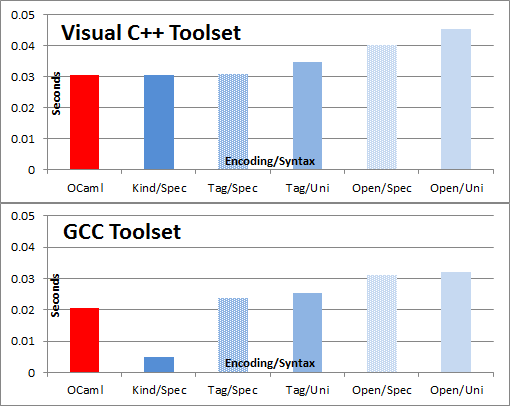
\includegraphics[width=0.47\textwidth]{OCamlComparison.png}
  \caption{Performance comparison of various encodings and syntax against OCaml code}
  \label{fig:OCamlComparison}
\end{figure}

We can see that the use of specialized syntax on a closed/sealed hierarchy can 
match the speed of, and even be four times faster than, the code generated by 
the native OCaml compiler. Once we go for an open solution, we become about 
30-50\% slower. 

\subsection{Qualitative Comparison}
\label{sec:qualcmp}

For this experiment we have reimplemented a visitor based C++ pretty printer for 
Pivot's IPR using our pattern matching library. Most of the rewrite was 
performed by sed-like replaces that converted visit methods into respective 
case-clauses. In several cases we had to manually reorder case-clauses to avoid 
redundancy as visit-methods for base classes were typically coming before the 
same for derived, while for pattern matching we needed them to come after. 
Redundancy checking support in the library discussed in \textsection\ref{sec:redun}
was invaluable in finding out all such cases.

During this refactoring we have made several simplifications that became obvious 
in pattern-matching code, but were not in visitors code because of control 
inversion. Simplifications that were applicable to visitors code were eventually 
integrated into visitors code as well to make sure we do not compare 
algorithmically different code. In any case we were making sure that both 
approaches regardless of simplifications were producing byte-to-byte the same 
output as the original pretty printer we started from.

The size of executable for pattern matching approach was smaller than that for 
visitors. So was also the source code. We extracted from both sources the 
functionality that was common to them and placed it in a separate translation 
unit to make sure it does not participate in the comparison. We kept all the 
comments however that were eqaully applicable to code in either approach.

Note that the visitors involved in the pretty printer above did not use 
forwarding: since all the C++ constructs were handled by the printer, every 
visit-method was overriden from those statically possible based on the static 
type of the argument.

%Listing parameter for a case clause always causes access to member. Best hope is 
%that compiler will eliminate it if it is not needed. At the moment we do not 
%have means to detect empty macro arguments or \_.

%To be continued...

In general from our rewriting experience we will not recommend rewriting 
existing visitor code with pattern matching for the simple reason that pattern 
matching code will likely follow the structure already set by the visitors. 
Pattern matching was most effective when writing new code, where we could design 
the structure of the code having the pattern matching facility in our toolbox.

\section{Related Work} %%%%%%%%%%%%%%%%%%%%%%%%%%%%%%%%%%%%%%%%%%%%%%%%%%%%%%%%%
\label{sec:rw}

There are two main approaches to compiling pattern matching code: the first is 
based on \emph{backtracking automata} and was introduced by Augustsson\cite{}, 
the second is based on \emph{decision trees} and is attributed in the literature 
to Dave MacQueen and Gilles Kahn in their implementation of Hope compiler \cite{}.
Backtracking approach usually generates smaller code, while decision tree 
approach produces faster code by ensuring that each primitive test is only 
performed once. Neither of the approaches addresses specifically type patterns 
or type switching and simply assumes presence of a primitive operation capable 
of performing type tests.

Memoization device we proposed is not specifically concerned with compiling 
pattern matching and can be used independently. In particular it can be combined 
with either backtracking or decision tree approaches to avoid subsequent 
decisions on datum that has already been seen.

%xxxxxxxxxxxxxxxxxxxxxxxxxxxxxxxxxxxxxxxxxxxxxxxxxxxxxxxxxxxxxxxxxxxxxxx

\emph{Extensible Visitors with Default Cases}~\cite[\textsection 
4.2]{Zenger:2001} attempt to solve the extensibility problem of visitors; 
however, the solution, after 
remapping it onto C++, has problems of its own. The visitation interface 
hierarchy can easily be grown linearly (adding new cases for the new classes in 
the original hierarchy each time), but independent extensions by different  
authorities require developer's intervention to unify them all, before they can 
be used together. This may not be feasible in environments that use dynamic 
linking. To avoid writing even more boilerplate code in new visitors, the 
solution would require usage of virtual inheritance, which typically has 
an overhead of extra memory dereferencing. On top of the double dispatch already 
present in the visitor pattern, the solution will incur two additional virtual 
calls and a dynamic cast for each level of visitor extension. Additional double 
dispatch is incurred by forwarding of default handling from a base visitor to a 
derived one, while the dynamic cast is required for safety and can be replaced 
with a static cast when the visitation interface is guaranteed to be grown linearly 
(extended by one authority only). Yet another virtual call is required to be 
able to forward computations to subcomponents on tree-like structures to the 
most derived visitor. This last function lets one avoid the necessity of using 
the heap to allocate a temporary visitor through the \emph{Factory Design 
Pattern}~\cite{DesignPatterns1993} used in the \emph{Extensible Visitor} solution 
originally proposed by Krishnamurti, Felleisen and Friedman~\cite{Krishnamurthi98}.

In order to address the expression problem in Haskell, L\"{o}h and Hinze proposed to 
extend its type system with open data types and open functions~\cite{LohHinze2006}.
Their solution allows the user to mark top-level data types and functions as 
open and then provide concrete variants and overloads anywhere in the program. 
Open data types are extensible but not hierarchical, which largely avoids the 
problems discussed here. The semantics of open extension is given by 
transformation into a single module, where all the definitions are seen in one 
place. This is a significant limitation of their approach that prevents it from 
being truly open, since it essentially assumes a whole-program view, which 
excludes any extension via DLLs. As is the case with many other implementations 
of open extensions, the authors rely on the closed world for efficient 
implementation: in their implementation, \emph{``data types can only be entirely 
abstract (not allowing pattern matching) or concrete with all constructors with 
the reason being that pattern matching can be compiled more efficiently if the 
layout of the data type is known completely''}. The authors also believe that 
\emph{there are no theoretical difficulties in lifting this restriction, but it 
might imply a small performance loss if closed functions pattern match on open 
data types}. Our work addresses exactly this problem, showing that it is not 
only theoretically possible but also practically efficient and in application to 
a broader problem.

Polymorphic variants in OCaml~\cite{garrigue-98} allow the addition of new variants 
later. They are simpler, however, than object-oriented extensions, as they do not 
form subtyping between variants themselves, but only between combinations of them. 
This makes an important distinction between \emph{extensible sum types} like 
polymorphic variants and \emph{extensible hierarchical sum types} like classes.
An important property of extensible sum types is that each value of the 
underlying algebraic data type belongs to exactly one disjoint subset, tagged with 
a constructor. The \emph{nominative subtyping} of object-oriented languages does 
not usually have this disjointness making classes effectively have multiple 
types. In particular, the case of disjoint constructors can be seen as a 
degenerated case of a flat class hierarchy among the multitude of possible class 
hierarchies.

\emph{Tom} is a pattern-matching compiler that can be used together with Java, C or 
Eiffel to bring a common pattern matching and term rewriting syntax into the 
languages\cite{Moreau:2003}. It works as a preprocessor that transforms 
syntactic extensions into imperative code in the target language. Tom is quite 
transparent as to the concrete target language used and can potentially be 
extended to other target languages besides the three supported now. In 
particular, it never uses any semantic information of the target language during 
the compilation process and it does not inspect nor modify the source language 
part (their preprocessor is only aware of parenthesis and block delimiters of 
the source language). Tom has a sublanguage called Gom that can be used to 
define algebraic data types in a uniform mannaer, which their preprocessor then 
transforms into conrete definitions in the target language. Alternatively, the 
user can provide mappings to his own data structures that the preprocessor will 
use to generate the code.

In comparison to our approach Tom has much bigger goals. The combination of 
pattern matching, term rewriting and strategies turns Tom into a 
tree-transformation language similar to Stratego/XT, XDuce and others. 
The main accent is made on expressivity and the speed of development, which 
makes one often wonder about the run-time complexity of the generated code.
Tom's approach is also prone to general problems of any preprocessor based 
solution\cite[\textsection 4.3]{SELL}. For example, when several preprocessors 
have to be used together, each independent extension may not be able to 
understand the other's syntax, making it impossible to form a toolchain.
A library approach we follow avoids most of these problems by relying only on a 
standard C++ compiler. It also lets us employ semantics of the language within 
patterns: e.g. our patterns work directly on underlying user-defined data 
structures, largely avoiding abstraction penalties. A tighter integration with 
the language semantics also makes our patterns first-class citizens that can be 
composed and passed to other functions. The approach we take to type switching 
can also be used by Tom's preprocessor to implement type patterns efficiently -- 
similarly to other object-oriented languages, Tom's handling of them is based on 
highly inefficient \code{instanceof} operator and its equivalents in other 
languages.

Pattern matching in Scala~\cite{Scala2nd} also allows type patterns and thus type 
switching. The language supports extensible and hierarchical data types, but 
their handling in a type switching constructs varies. Sealed classes are handled 
with an efficient switch over all tags, since sealed classes cannot be extended. 
Classes that are not sealed are similarly approached with a combination of an 
\code{InstanceOf} operator and a decision tree~\cite{EmirThesis}.

%An example would be our generalized n+k patterns where we 
%can turn any invertible function even user defined into a pattern.

There has been previous attempts to use pattern matching with the Pivot 
framework that we used to experiment with our library. In his dissertation, 
Pirkelbauer devised a pattern language capable of representing various entities 
in a C++ program. The patterns were then translated with a tool into a set of 
visitors implementing the underlying pattern matching 
semantics\cite{PirkelbauerThesis}. Earlier, Cook et al used expression templates 
to implement a query language for Pivot's Internal Program Representation 
\cite{iql04}. While their work was built around a concrete class hierarchy 
letting them put some semantic knowledge about concrete classes into the 
The principal difference of their work from this work is that 
authors were essentially creating a pattern matcher for a given class hierarchy 
and thus could take the semantics of the entities represented by classes in the 
hierarchy into account. Our approach is parametrized over class hierarchy and 
thus provides a rather lower level pattern-matching functionality that lets one 
simplify work with that hierarchy.  One can think of it as a generalized 
dynamic\_cast. To be continued...

\section{Future Work} %%%%%%%%%%%%%%%%%%%%%%%%%%%%%%%%%%%%%%%%%%%%%%%%%%%%%%%%%%
\label{sec:fw}

In the future we would like to provide an efficient multi-threaded 
implementation of our library as currently it relies heavily on static variables 
and global state, which will have problems in a multi-threaded environment. 

The match statement that we presented here deals with only one subject at the 
moment, but we believe that our memoization device, along with the vtable pointer memoization 
technique we presented, can cope reasonably efficiently with multiple subjects. 
Their support will make our library more general by addressing asymmetric 
multiple dispatch.

We would also like to experiment with other kinds of cache indexing functions in 
order to decrease the frequency of conflicts, especially those coming from the use 
of dynamically-linked libraries.

Containers as described by the standard C++ library do not have the implicit 
recursive structure present in lists, sequences and other recursive data 
structures of functional languages. Viewing them as such with view will likely 
have a significant performance overhead, not usually affordable in the kind of 
applications C++ is used for. We therefore would like to experiment with some 
pattern matching alternatives that will let us work with STL containers 
efficiently yet expressively as in functional languages.

\section{Conclusions} %%%%%%%%%%%%%%%%%%%%%%%%%%%%%%%%%%%%%%%%%%%%%%%%%%%%%%%%%%
\label{sec:cc}

Type switching is an open alternative to visitor design pattern that overcomes 
the restrictions, inconveniences, and difficulties in teaching and using, 
typically associated with it. Our implementation of it comes close or 
outperforms the visitor design pattern, which is true even in a library setting 
using a production-quality compiler, where the performance base-line is 
already very high.

We describe three techniques that can be used to implement type switching, type 
testing, pattern matching, predicate dispatching, and other facilities that 
depend on the run-time type of an argument as well as demonstrate their efficiency.

The \emph{Memoization Device} is an optimization technique that maps run-time values 
to execution paths, allowing to take shortcuts on subsequent runs with the same 
value. The technique does not require code duplication and in typical cases adds 
only a single indirect assignment to each of the execution paths. It can be 
combined with other compiler optimizations and is particularly suitable for use 
in a library setting.

The \emph{Vtable Pointer Memoization} is a technique based on memoization device that 
employs uniqueness of virtual table pointers to not only speed up execution, but 
also properly uncover the dynamic type of an object. This technique is a 
backbone of our fast type switch as well as memoized dynamic cast optimization.

The \emph{TPL Dispatcher} is yet another technique that can be used to 
implement best-fit type switching on tagged classes. The technique has its pros 
and cons in comparison to vtable pointer memoization, which we discuss in the paper.

These techniques can be used in a compiler and library setting, and support well 
separate compilation and dynamic linking. They are open to class extensions and 
interact well with other C++ facilities such as multiple inheritance and 
templates. The techniques are not specific to C++ and can be adopted in other 
languages for similar purposes.

Using the above techniques, we implemented a library for efficient type switching 
in C++. We used the library to rewrite existing code that relied heavily on 
visitors, and discovered that the resulting code became much shorter, simpler, 
and easier to maintain and comprehend.

We used the library to rewrite existing code that relied heavily on 
visitors, and discovered that the resulting code became much shorter, simpler, and easier 
to maintain and comprehend.

\bibliographystyle{abbrvnat}
\bibliography{mlpatmat}
\end{document}
